\chapter{Local and Non-local Analyses of Natural Images}\label{chap:chapter3}
\graphicspath{{Chapter3/}}

Neuroscientists have a long-standing and challenging question: how does HVS evaluate perceptual quality without reference images? In other words, is there an ideal observer,~\ie, a perceptual optimization objective, of image quality with regard to early human vision? Human-centered evaluation of image quality has dominated the field over decades~\footnote{~In this thesis, we assume that the ultimate destination of image quality is human eyes (biological vision) instead of machines (machine vision).}. Simulating how HVS perceives and processes visual signals is one of the mainstreams of IQA. Thus, most previous works originate from HVS in which they imitate the biological signal processing mechanisms and basic characteristics of HVS.

Both local and non-local features contribute to image quality assessment~\citep{golestaneh2021no}. In~\citep{zhao2021battle}, Zhao~\etal empirically suggest that the local modeling is robust and efficient for various CV tasks. Our experiments have shown similar results and findings where we also discover that the non-local modeling is a supplemental element, which enhances representation ability and promotes prediction performance~\citep{wang2018non, liu2020long}. In the following sections, the local modeling analyses and non-local modeling analyses of natural images are summarized.

\section{Local Modeling Analyses of Natural Images}\label{Local Modeling Analyses of Natural Images}
Over the past two decades, the most convincing and successful models have been built upon the Classical feedforward Receptive Field (CRF) in HVS, discovered by observing cats' primary visual cortex~\emph{in~situ} by Dr.~David Hubel and Dr.~Torsten Wiesel~\citep{hubel1968receptive}. It has been one of the most influential biological mechanisms in the field, such as neuroscience, psychophysiology, physiology, and visual processing. Inspired by the CRF, numerous computational models of HVS are put forward to model local pixels' spatial dependencies. Among these local-modeling methods, CNN is insanely effective and efficient, and the ``unreasonable'' effectiveness of deep feature representation has triggered attention of researchers and engineers in academia and industry~\citep{lecun1998gradient, zhang2018unreasonable, SimonyanZ14a, dingIQA}. It is broadly applied to CV tasks based on the inductive biases of images, such as locality and spatial invariance~\citep{SimonyanZ14a}. 

The local modeling encodes spatially proximate local neighborhoods. The CNN-based local modeling features are critical and robust~\citep{zhang2018unreasonable, ding2021comparison, dingIQA}. First, pixels in a local region are spatially proximate with high spatial correlation as local regions are usually piecewise smooth~\citep{mittal2012no}. The strong dependencies among neighborhood pixels carry essential information about the structure of objects. HVS is adapted to extract such structural information and is sensitive to visible structural distortions~\citep{wang2004image}. Besides, image degradation may be space-variant, and image statistics are typically spatially non-stationary~\citep{sun2018spsim}. It is much more accurate to explore features within a local region. Furthermore, the overall image quality affects quality assessment. So do local appearance artifacts, as HVS is adaptive to the local content~\citep{liu2020long, wang2005adaptive}. Last but not least, since image quality is degraded hierarchically, the local modeling learns the hierarchical degraded features from the low-level local details degradation, middle-level regional patterns degradation, to the high-level global abstract degradation, inspired by the hierarchical perception mechanism in HVS~\citep{wu2020end}. Thus, obtaining features from local regions is of great essence. In Chapter~\ref{chap:chapter4}, we conduct an ablation study to explore the contribution of the local modeling to visual quality assessment. It has achieved 0.936 PLCC and 0.951 SRCC on the CSIQ database~\citep{larson2010most}~\footnote{~PLCC stands for Pearson Linear Correlation Coefficient, which measures prediction accuracy. SRCC is the Spearman Rank-order Correlation Coefficient and measures prediction monotonicity.}. Experimental results have verified the effectiveness and robustness of CNN's local modeling features in measuring perceptual quality. However, although CNN has achieved encouraging results, there are still some spaces to improve it.

%	\subsection{Extracted Features are Too Local}\label{Extracted Features are too Local}
%	CNN captures long-range dependencies via a hierarchical architecture. However, it shows that the non-local modeling ability through the cascaded convolutional and pooling layers is poor and inefficient under the principle of local processing~\citep{wang2018non}. In addition, there is a relatively small-sized receptive field with the local convolutional operation, which mainly extracts local features from local neighborhoods. Some works have advised employing a somewhat larger receptive field or deformable convolutional kernel to take the benefit from context information~\citep{szegedy2015going, dai2017deformable}. Nevertheless, it is still challenging to catch the non-local features and long-range dependencies among pixels and regions from the image~\citep{wang2018non}.
	
%	\subsection{Content is Equally Treated}\label{Content is Equally Treated}
%	The parameters of CNN are fixed and shared across the whole image after training. There are several advantages to the sliding window operation and weight sharing, such as translation equivalence and fewer trainable parameters. However, considering different contexts in images are treated equally, it is unable to capture the unique content and global context dependencies among objects in the image~\citep{yue2018compact}. Besides, multi-scale spatial visual processing is a kind of HVS characteristic. The content in an image is naturally multi-scale. Thus, feature interactions among scales should be content-adaptive and flexible rather than equal treatment~\citep{wang2003multiscale}.
	
%	\subsection{Lack of Geometric and Relational Modeling}\label{Lack of Geometrical and Relational Modeling}
%	Local content's non-local information and long-range dependencies can model complex relations and layouts inside an image~\citep{she2021hierarchical}. As suggested in reference~\citep{wang2018non}, the mechanism of non-local behavior is vital to the network to learn meaningful and valuable relational and causal dependencies not only in space but also in time. However, for CNN models, relational clues and global interactions between different regions are hard to learn. Moreover, geometric and structural patterns that occur consistently are also missing~\citep{zhang2019self}.

\section{Non-local Modeling Analyses of Natural Images}\label{Non-local Modeling Analyses for Natural Images}
	The biological foundation of the non-local modeling lies in the Non-classical Receptive Field (nCRF), a remotely placed and larger region around the CRF in the primary visual cortex of HVS~\citep{polat1996neurophysiological, zenger1996isolating}. The non-local modeling establishes the spatial integration of information by long- and short-range communications with different spatial weighting functions. Thus, an attention-based non-local block can be employed to simulate the spatial weighting functions as they compute a weighted sum of all information among signals or regions~\citep{wang2018non, buades2011non, vaswani2017attention}. There are different types of weighting functions, such as Gaussian, Embedded Gaussian, self-attention, dot-product, and concatenation~\citep{wang2018non}. Linking these widely separated visual fields integrates stimulus information and delivers a much more comprehensive and robust representation to process visual signals~\citep{polat1996neurophysiological}. We also unilaterally implement the non-local modeling for visual quality prediction, which has obtained 0.625 PLCC and 0.577 SRCC performances. In addition, the effectiveness of the non-local modeling is further verified by combining two modeling methods. It has achieved superior performances to the models utilized individually. Overall, the ablation study has demonstrated the complementary role of local and non-local modelings, and superior performances can be achieved by combining the two types of methods. The following are some non-local modeling analyses of natural images.
	
	\subsection{Non-local Statistics}\label{Non-local Statistics}
	Zontak~\etal discover that the non-local features, measured by spatial distance and gradient content, are a kind of internal statistics of natural images,~\ie, NSS~\citep{zontak2011internal, irani2019blind, zontak2018internal, zhu2003statistical}. Thus, the non-local statistics are perceptually relevant to HVS~\citep{irani2019blind}. It also explains that this internal image-specific prior holds strong prediction power and expressiveness~\citep{zontak2011internal, irani2019blind, zontak2018internal, zhang2010non}. Based on this work, the non-local modeling is employed to a wide variety of CV tasks, such as image denoising~\citep{buades2011non, mosseri2013combining, zontak2013separating}, texture manipulation~\citep{dekel2015revealing}, super-resolution~\citep{wang2015learning, freedman2011image, zuckerman2020across, cheng2020zero}, deblurring~\citep{michaeli2014blind}, and matching local similarities~\citep{shechtman2007matching}. 
	
	In addition, the non-local means (NL-means), a type of NSS, take full advantage of all possible recurrent patches and pixels and compute a weighted average of all pixels in an image. The filtered response in a local region is contributed not only by pixels inside the local region but also by distant pixels based on their appearance similarity~\citep{buades2011non}.
	
	\subsection{Non-local Dependency and Relational Modeling}\label{Non-local Dependency and Relational Modeling}
	The semantic and content understanding for relationship modeling is increasingly essential for modern CV tasks~\citep{hu2018relation}. The relationship modeling of basic visual elements consists of pixel-to-pixel modeling, object-to-pixel modeling, and object-to-object modeling. The pixel-to-pixel modeling is usually achieved by convolutions or self-attention during the image feature extraction process~\citep{wang2018non, yin2020disentangled, hu2019local, cao2019gcnet}. Region of Interest Align (RoIAlign) or self-attention mechanism is applied to model object-to-pixel associations via region feature extraction~\citep{gu2018learning, chi2020relationnet}. Lastly, the object-to-object connections are modeled by separate object analyses in the region head, where the self-attention mechanism can also be employed~\citep{hu2018relation}.
	
	\textit{De~facto}, the non-local modeling plays an essential role in modeling dependencies and relations in images or videos~\citep{wang2018non}. In~\reffig{Non-local Behavior from the TID2013 database}, we illustrate the non-local behavior of long-range dependencies and relations by randomly taking examples from the TID2013~\citep{ponomarenko2015image}, CSIQ~\citep{larson2010most}, and LIVE~\citep{livedataset} databases. The red dot is a query point (reference position), and the blue lines are queries' non-local responses achieved by the proposed NLNet. The line width denotes the attentional weight. To demonstrate the effectiveness of the non-local modeling and for better visibility, we resize the original image into $112~\times~112$.
	\begin{figure}[ht]
		\centering
		\begin{minipage}[t]{.32\linewidth}
			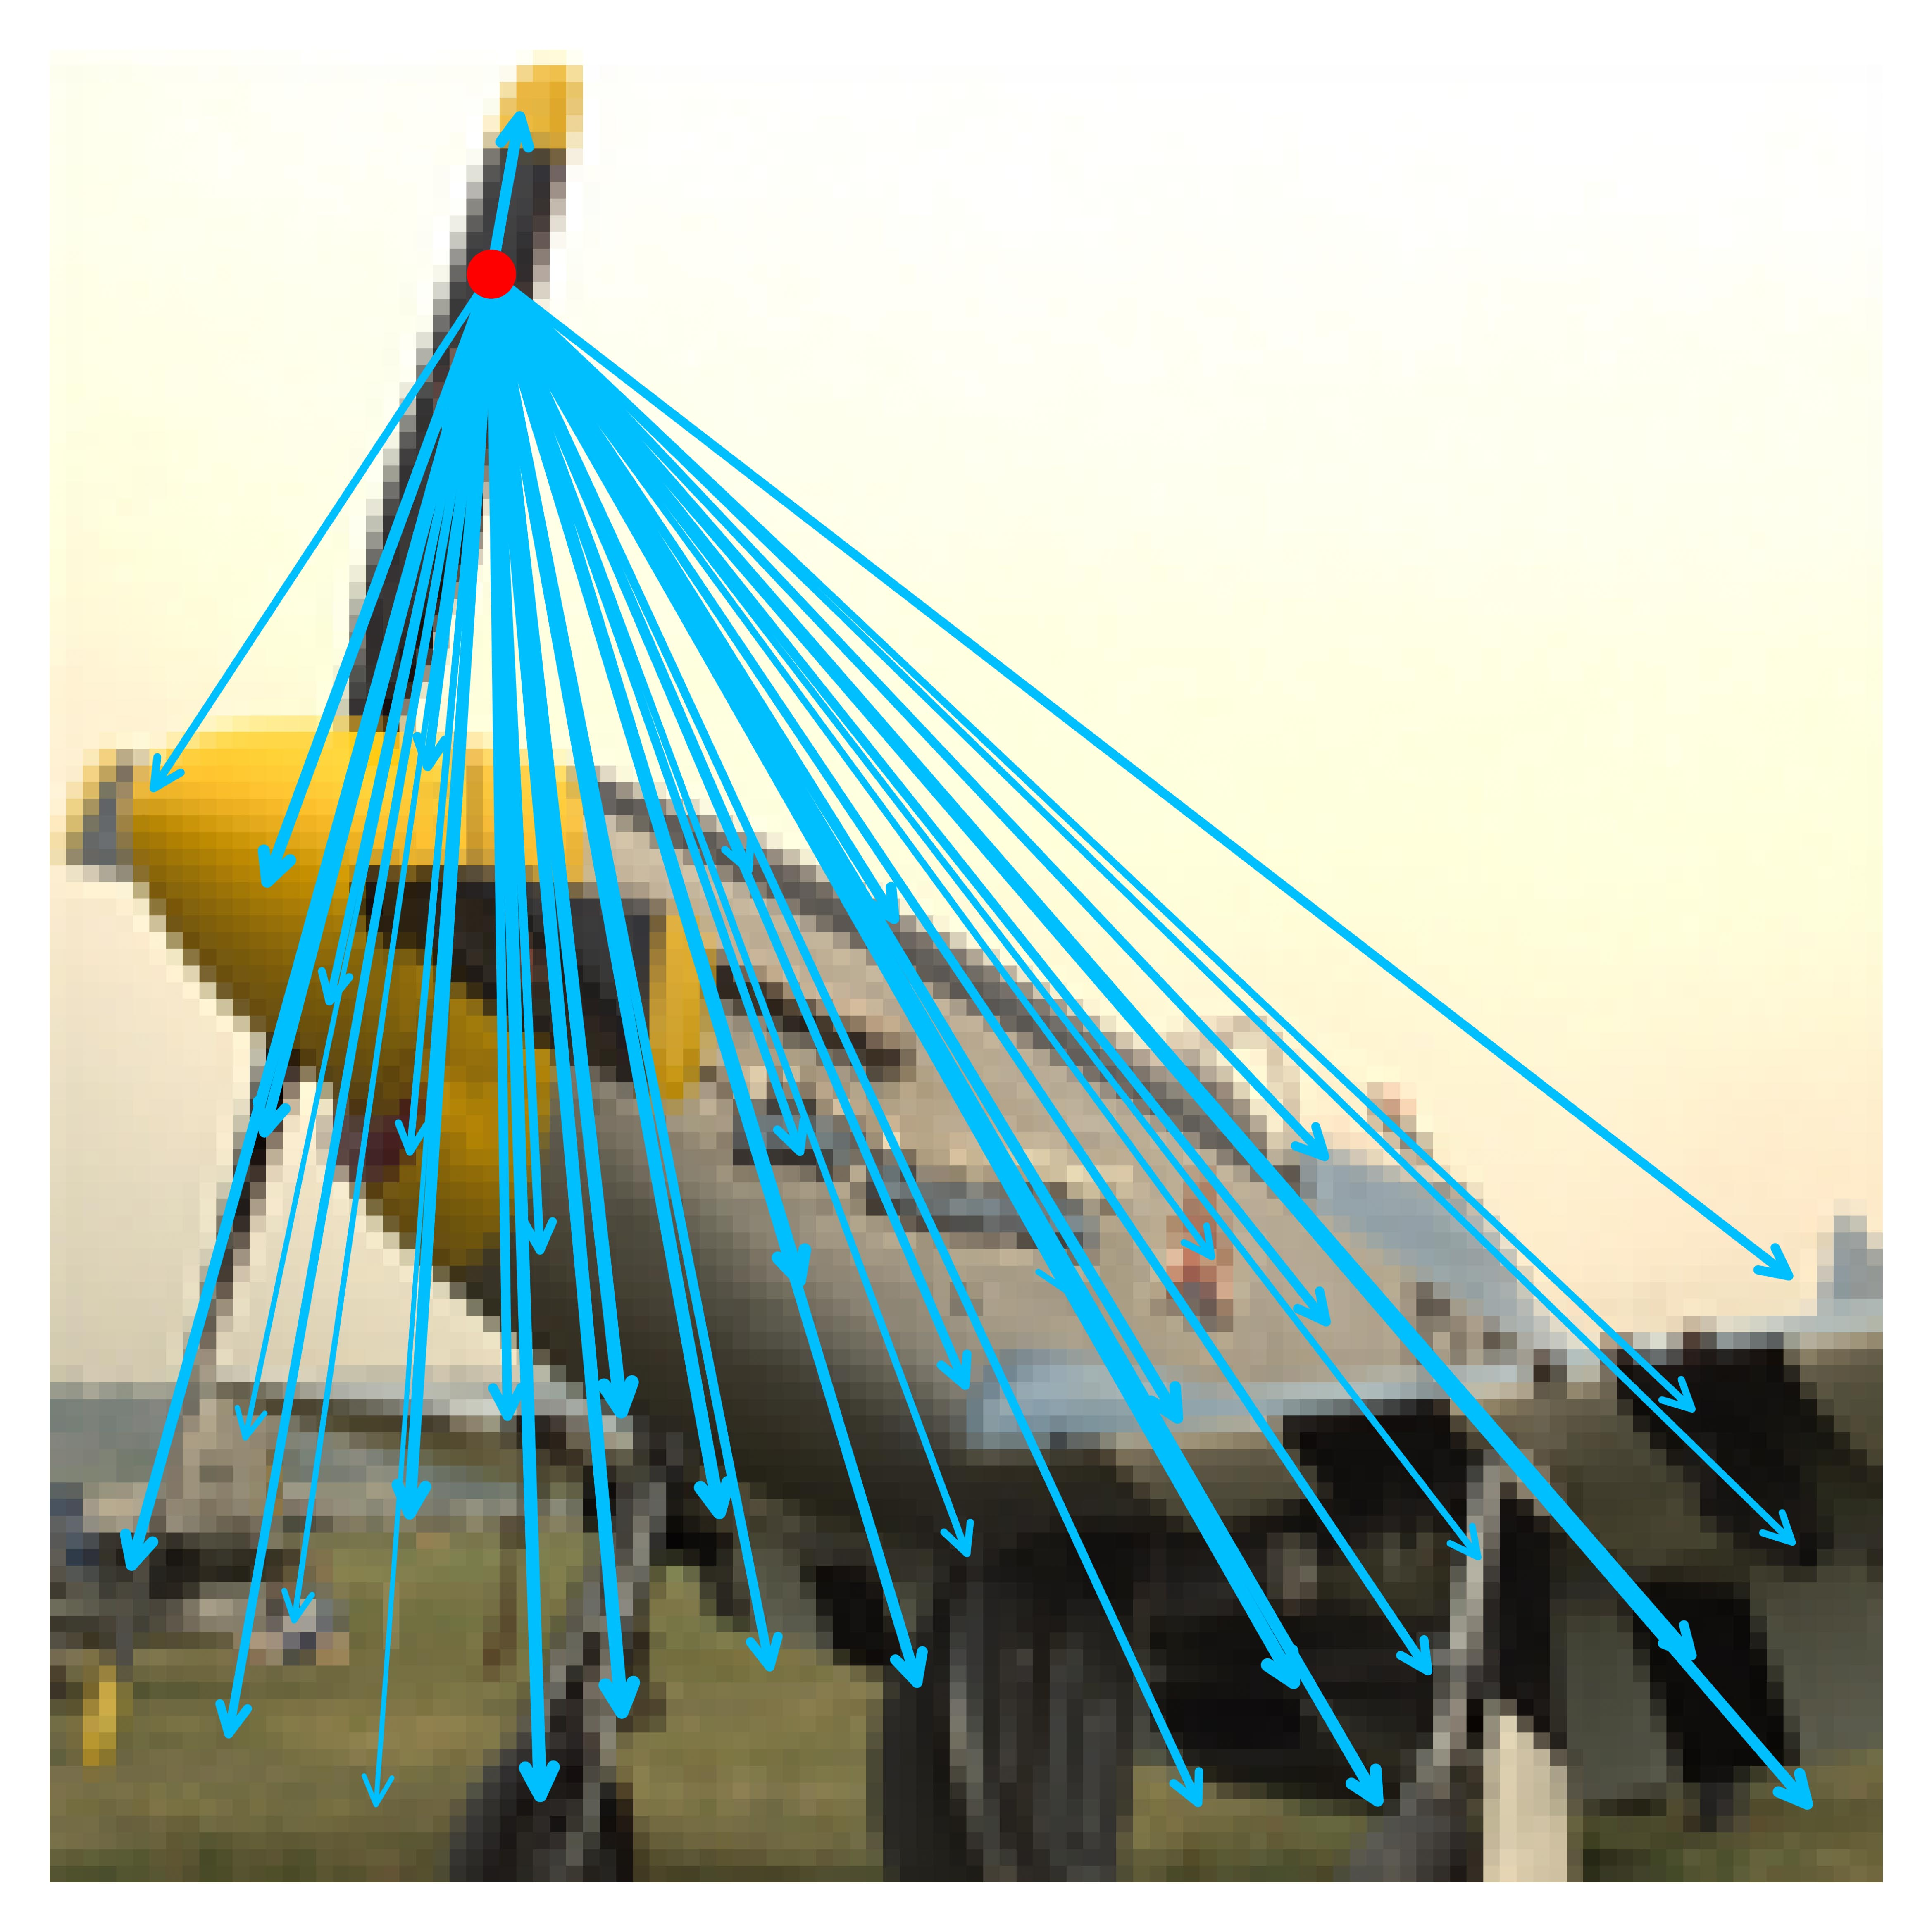
\includegraphics[width=1.9in]{fig/jet_superpixel_crop.jpg}
			\centerline{(a)}
		\end{minipage}
		\begin{minipage}[t]{.32\linewidth}
			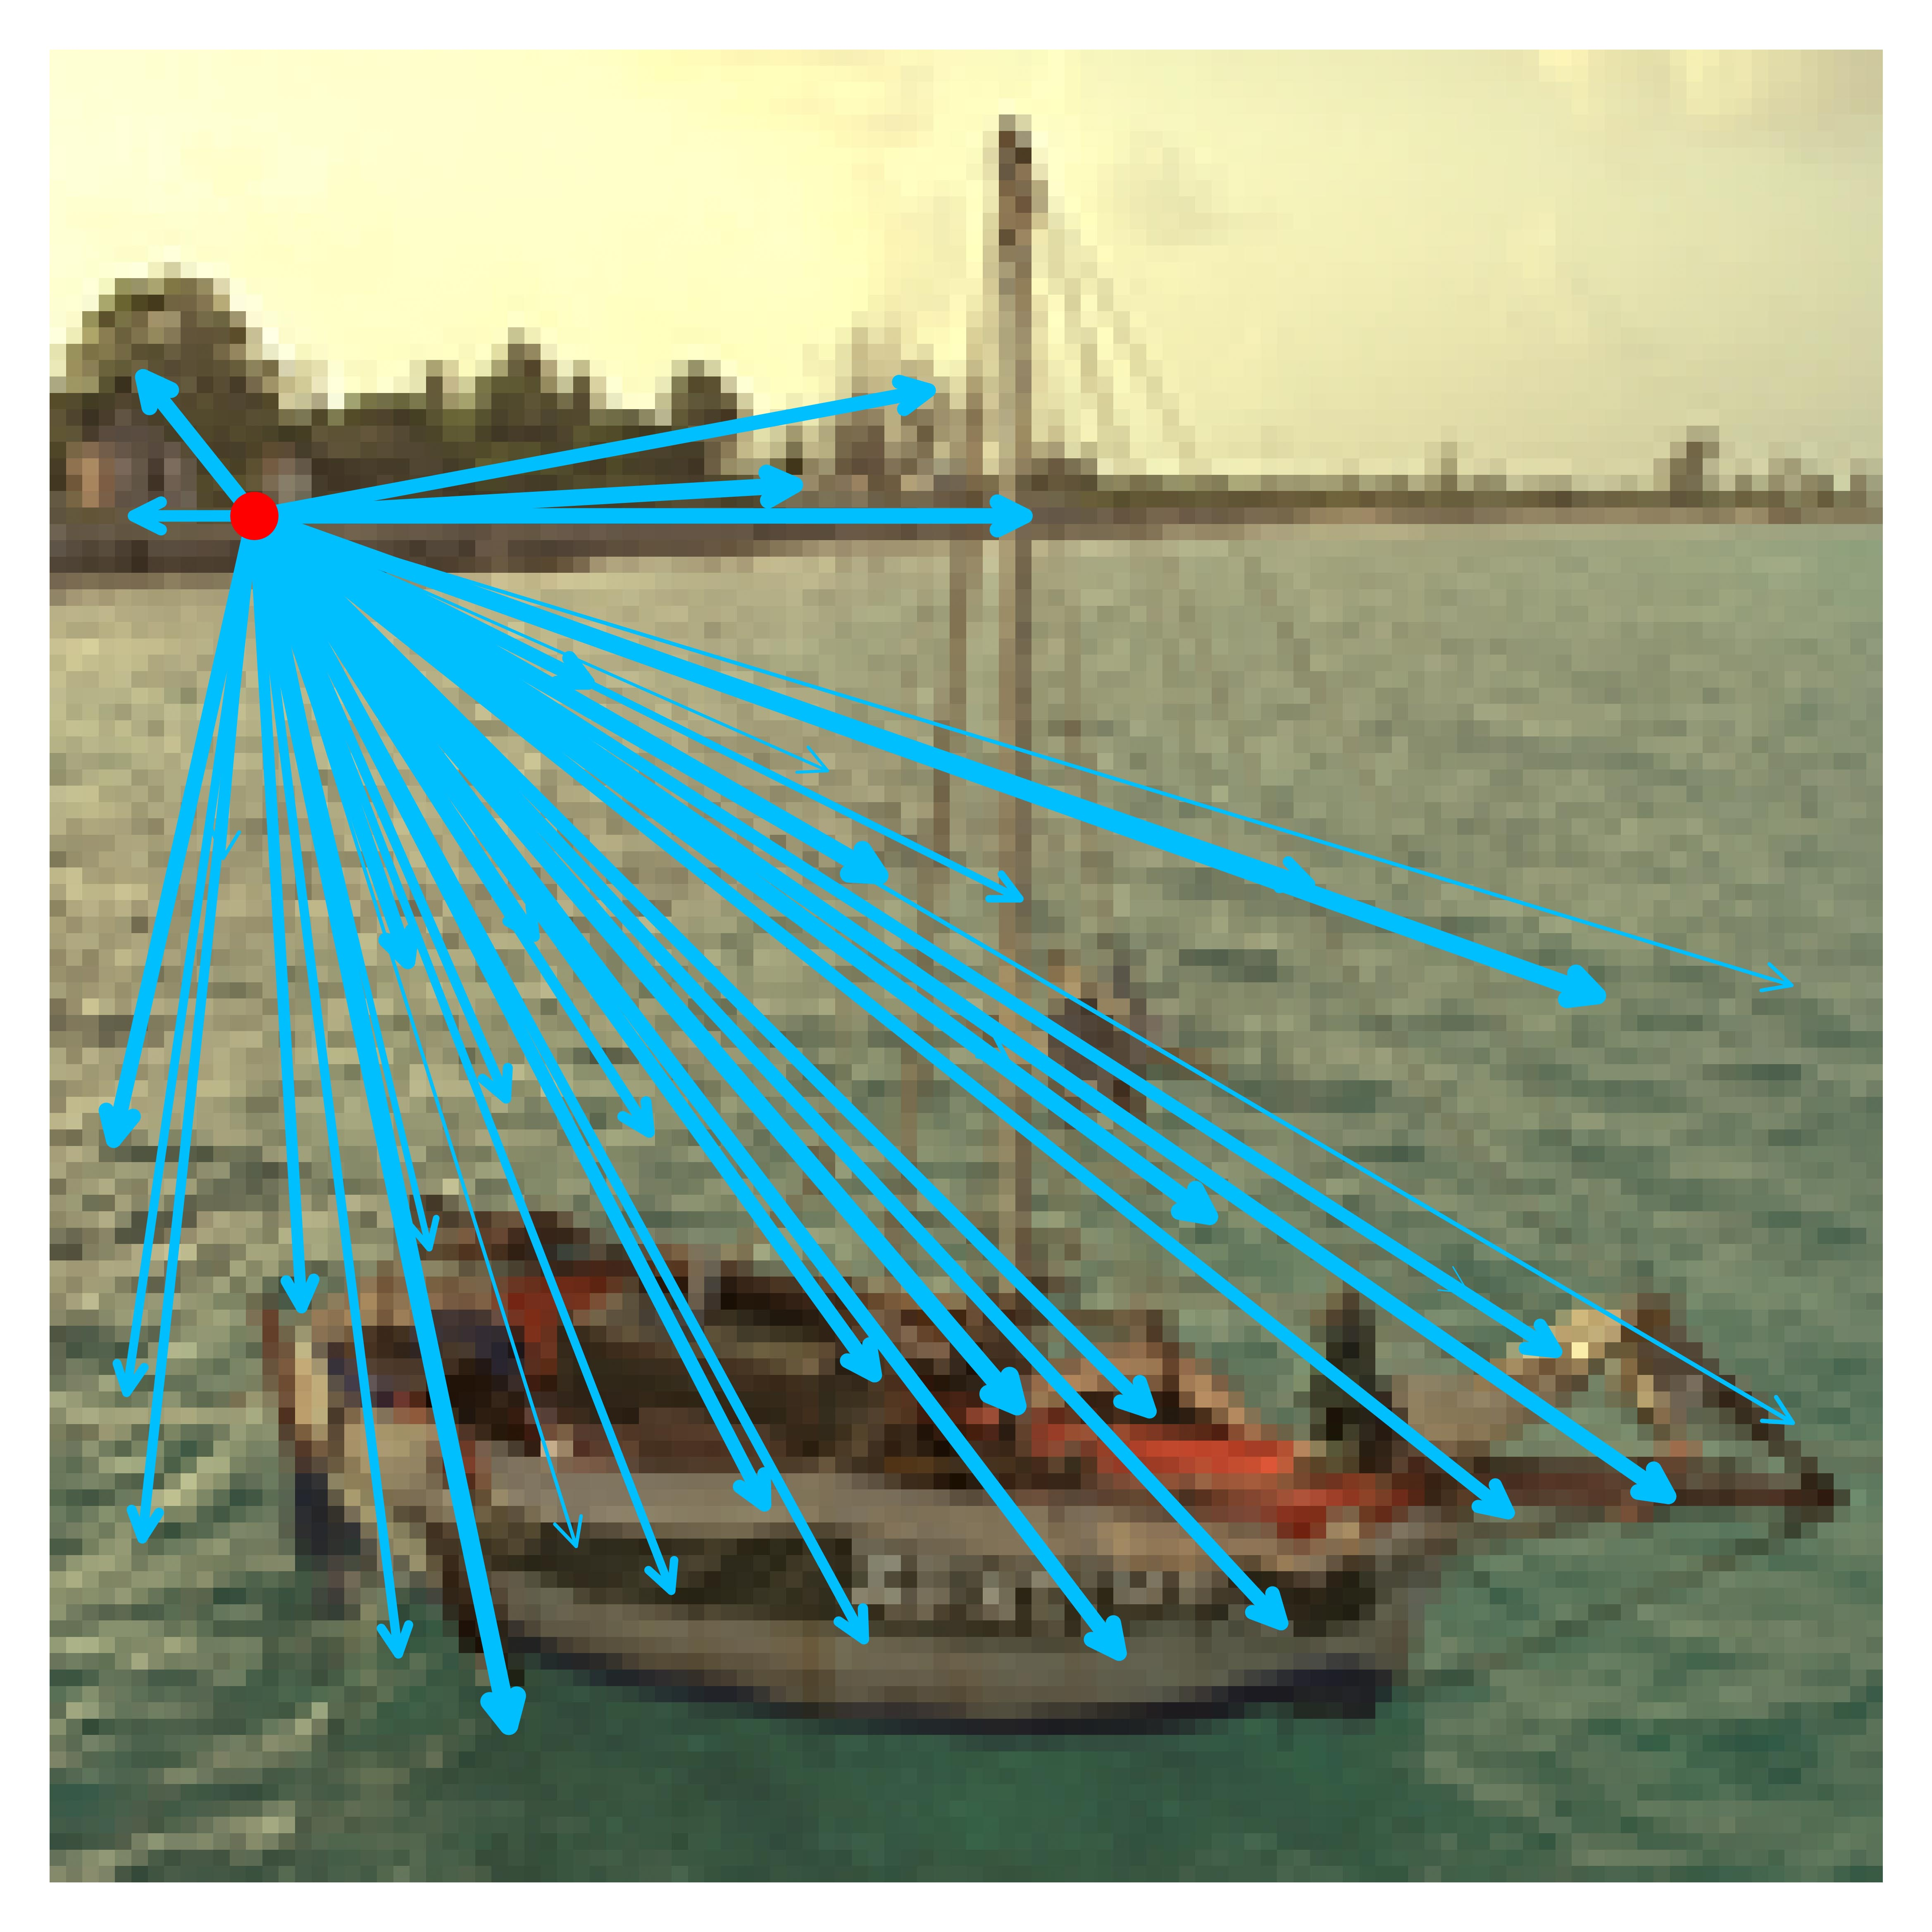
\includegraphics[width=1.9in]{fig/I06_superpixel.jpg}
			\centerline{(b)}
		\end{minipage}
		\begin{minipage}[t]{.32\linewidth}
			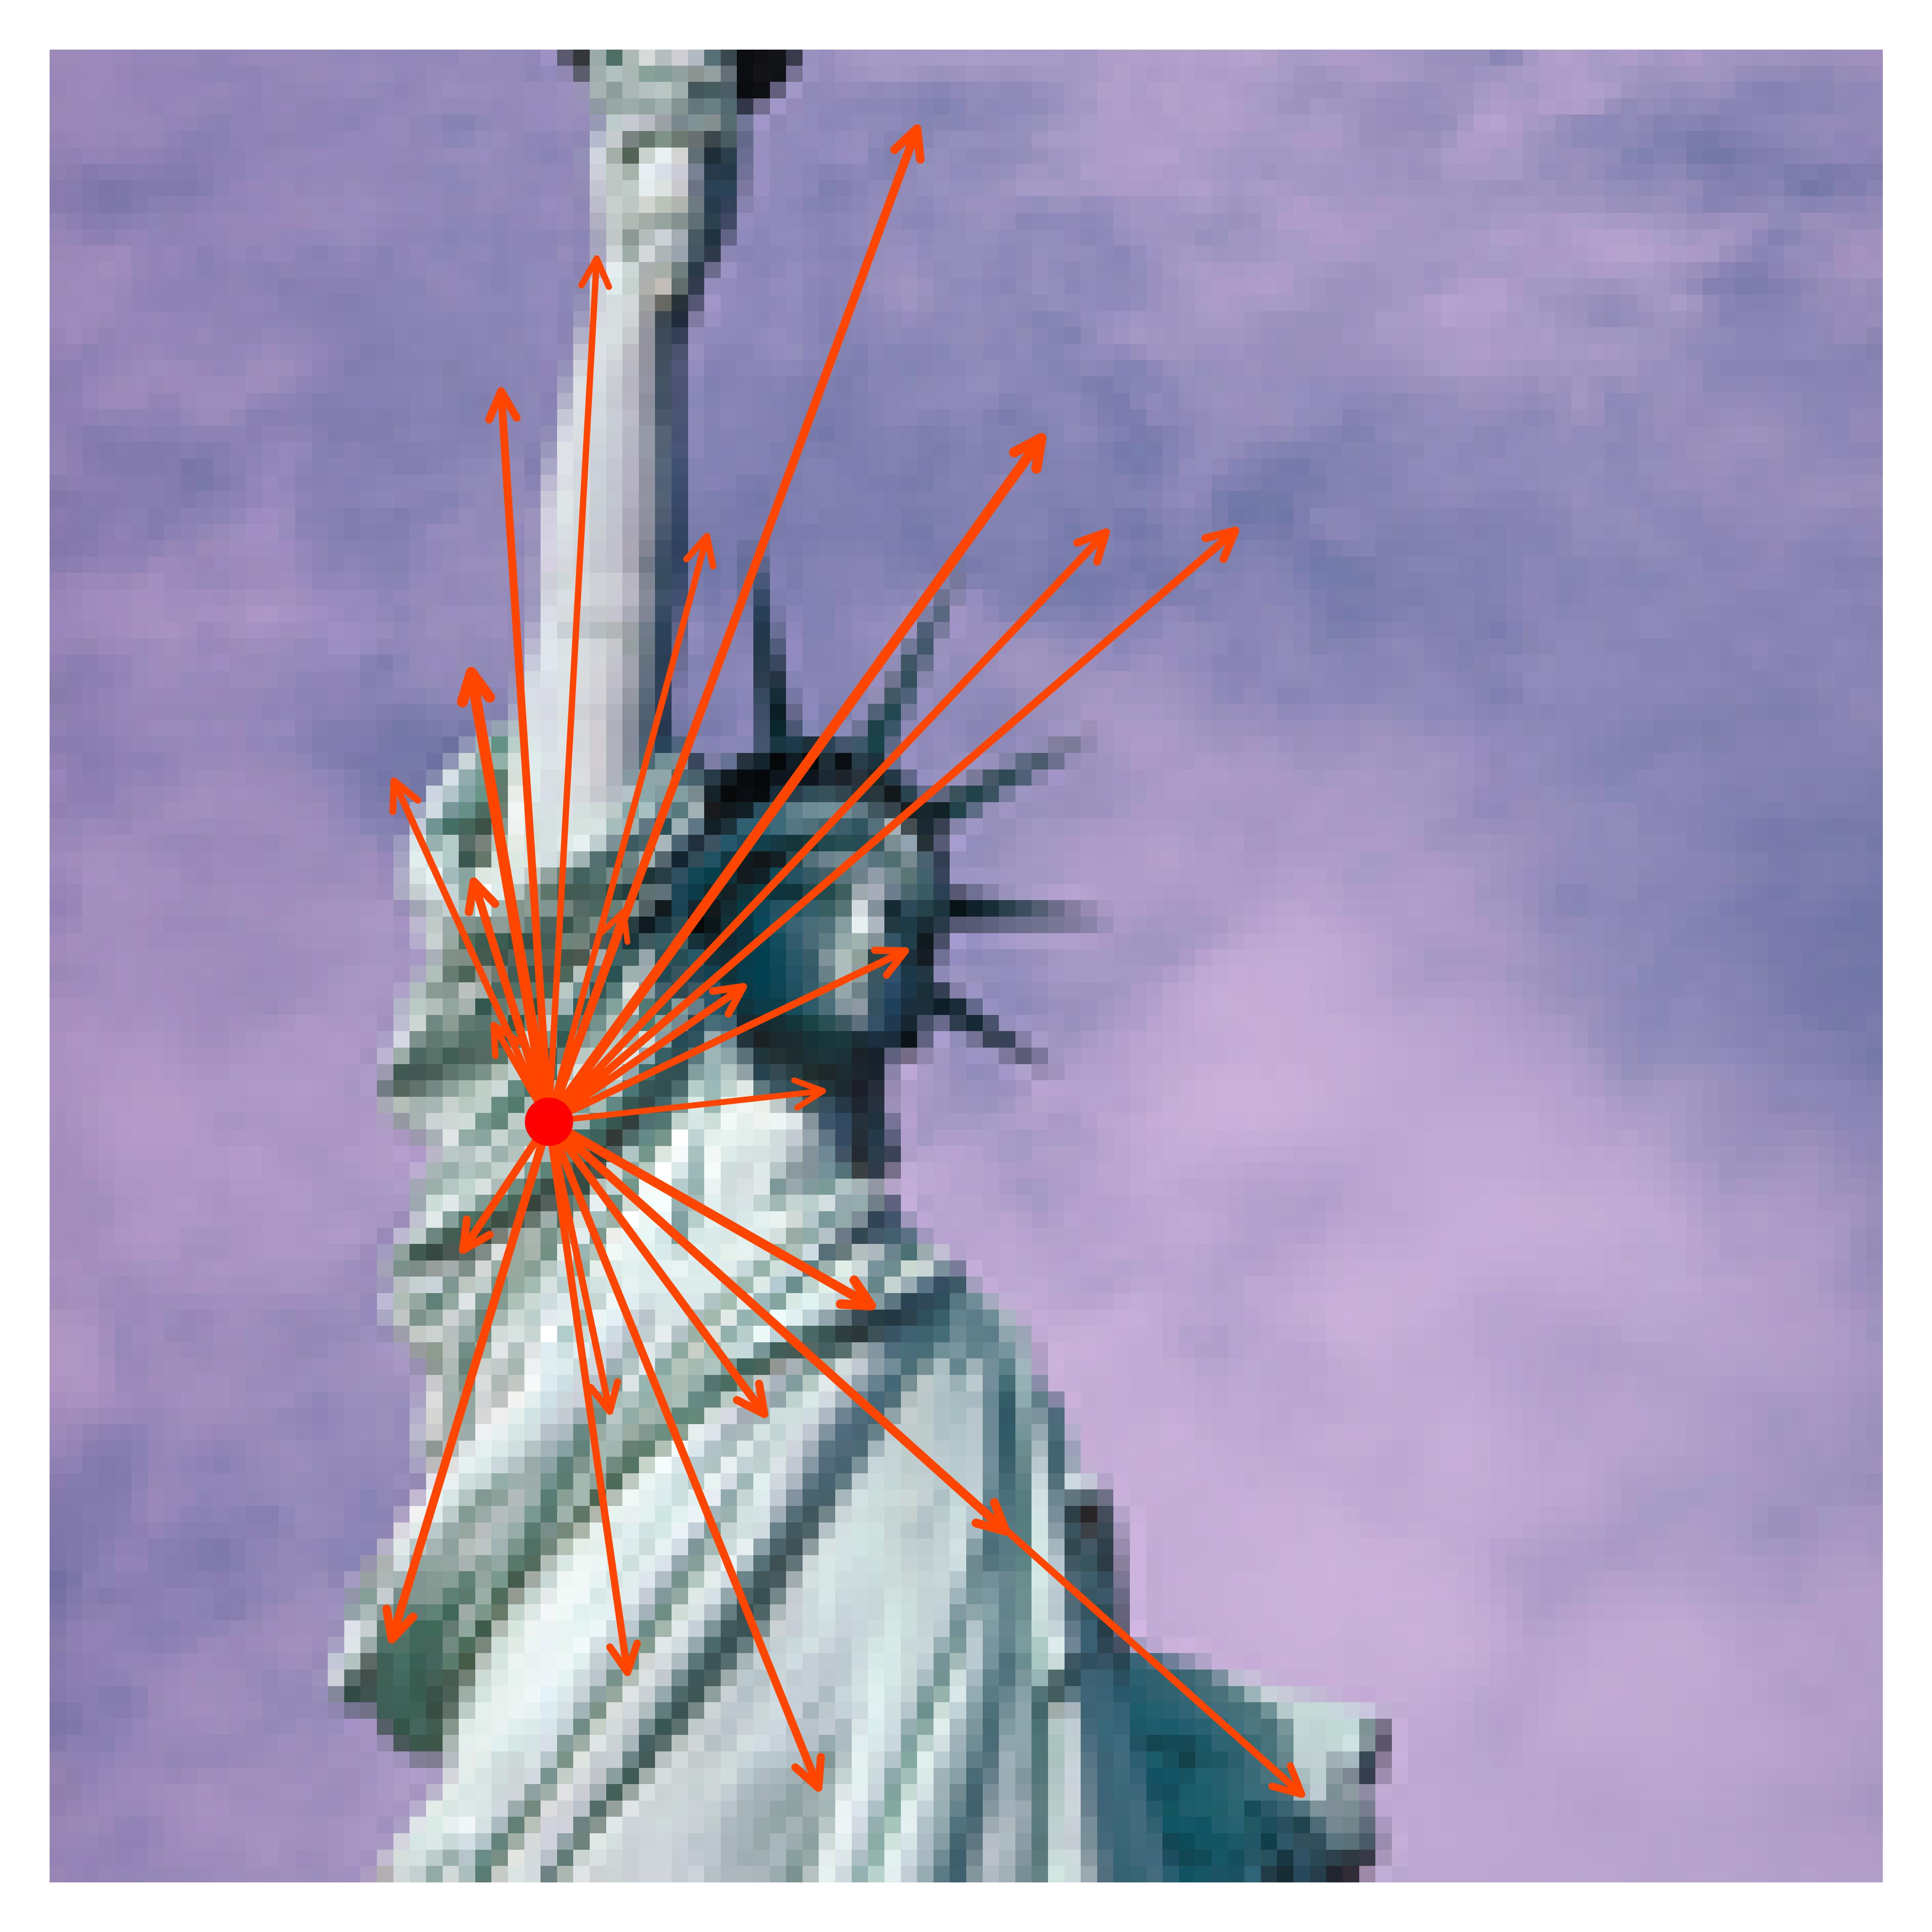
\includegraphics[width=1.9in]{fig/lady_superpixel.jpg}
			\centerline{(c)}
		\end{minipage}
		\begin{minipage}[t]{.32\linewidth}
			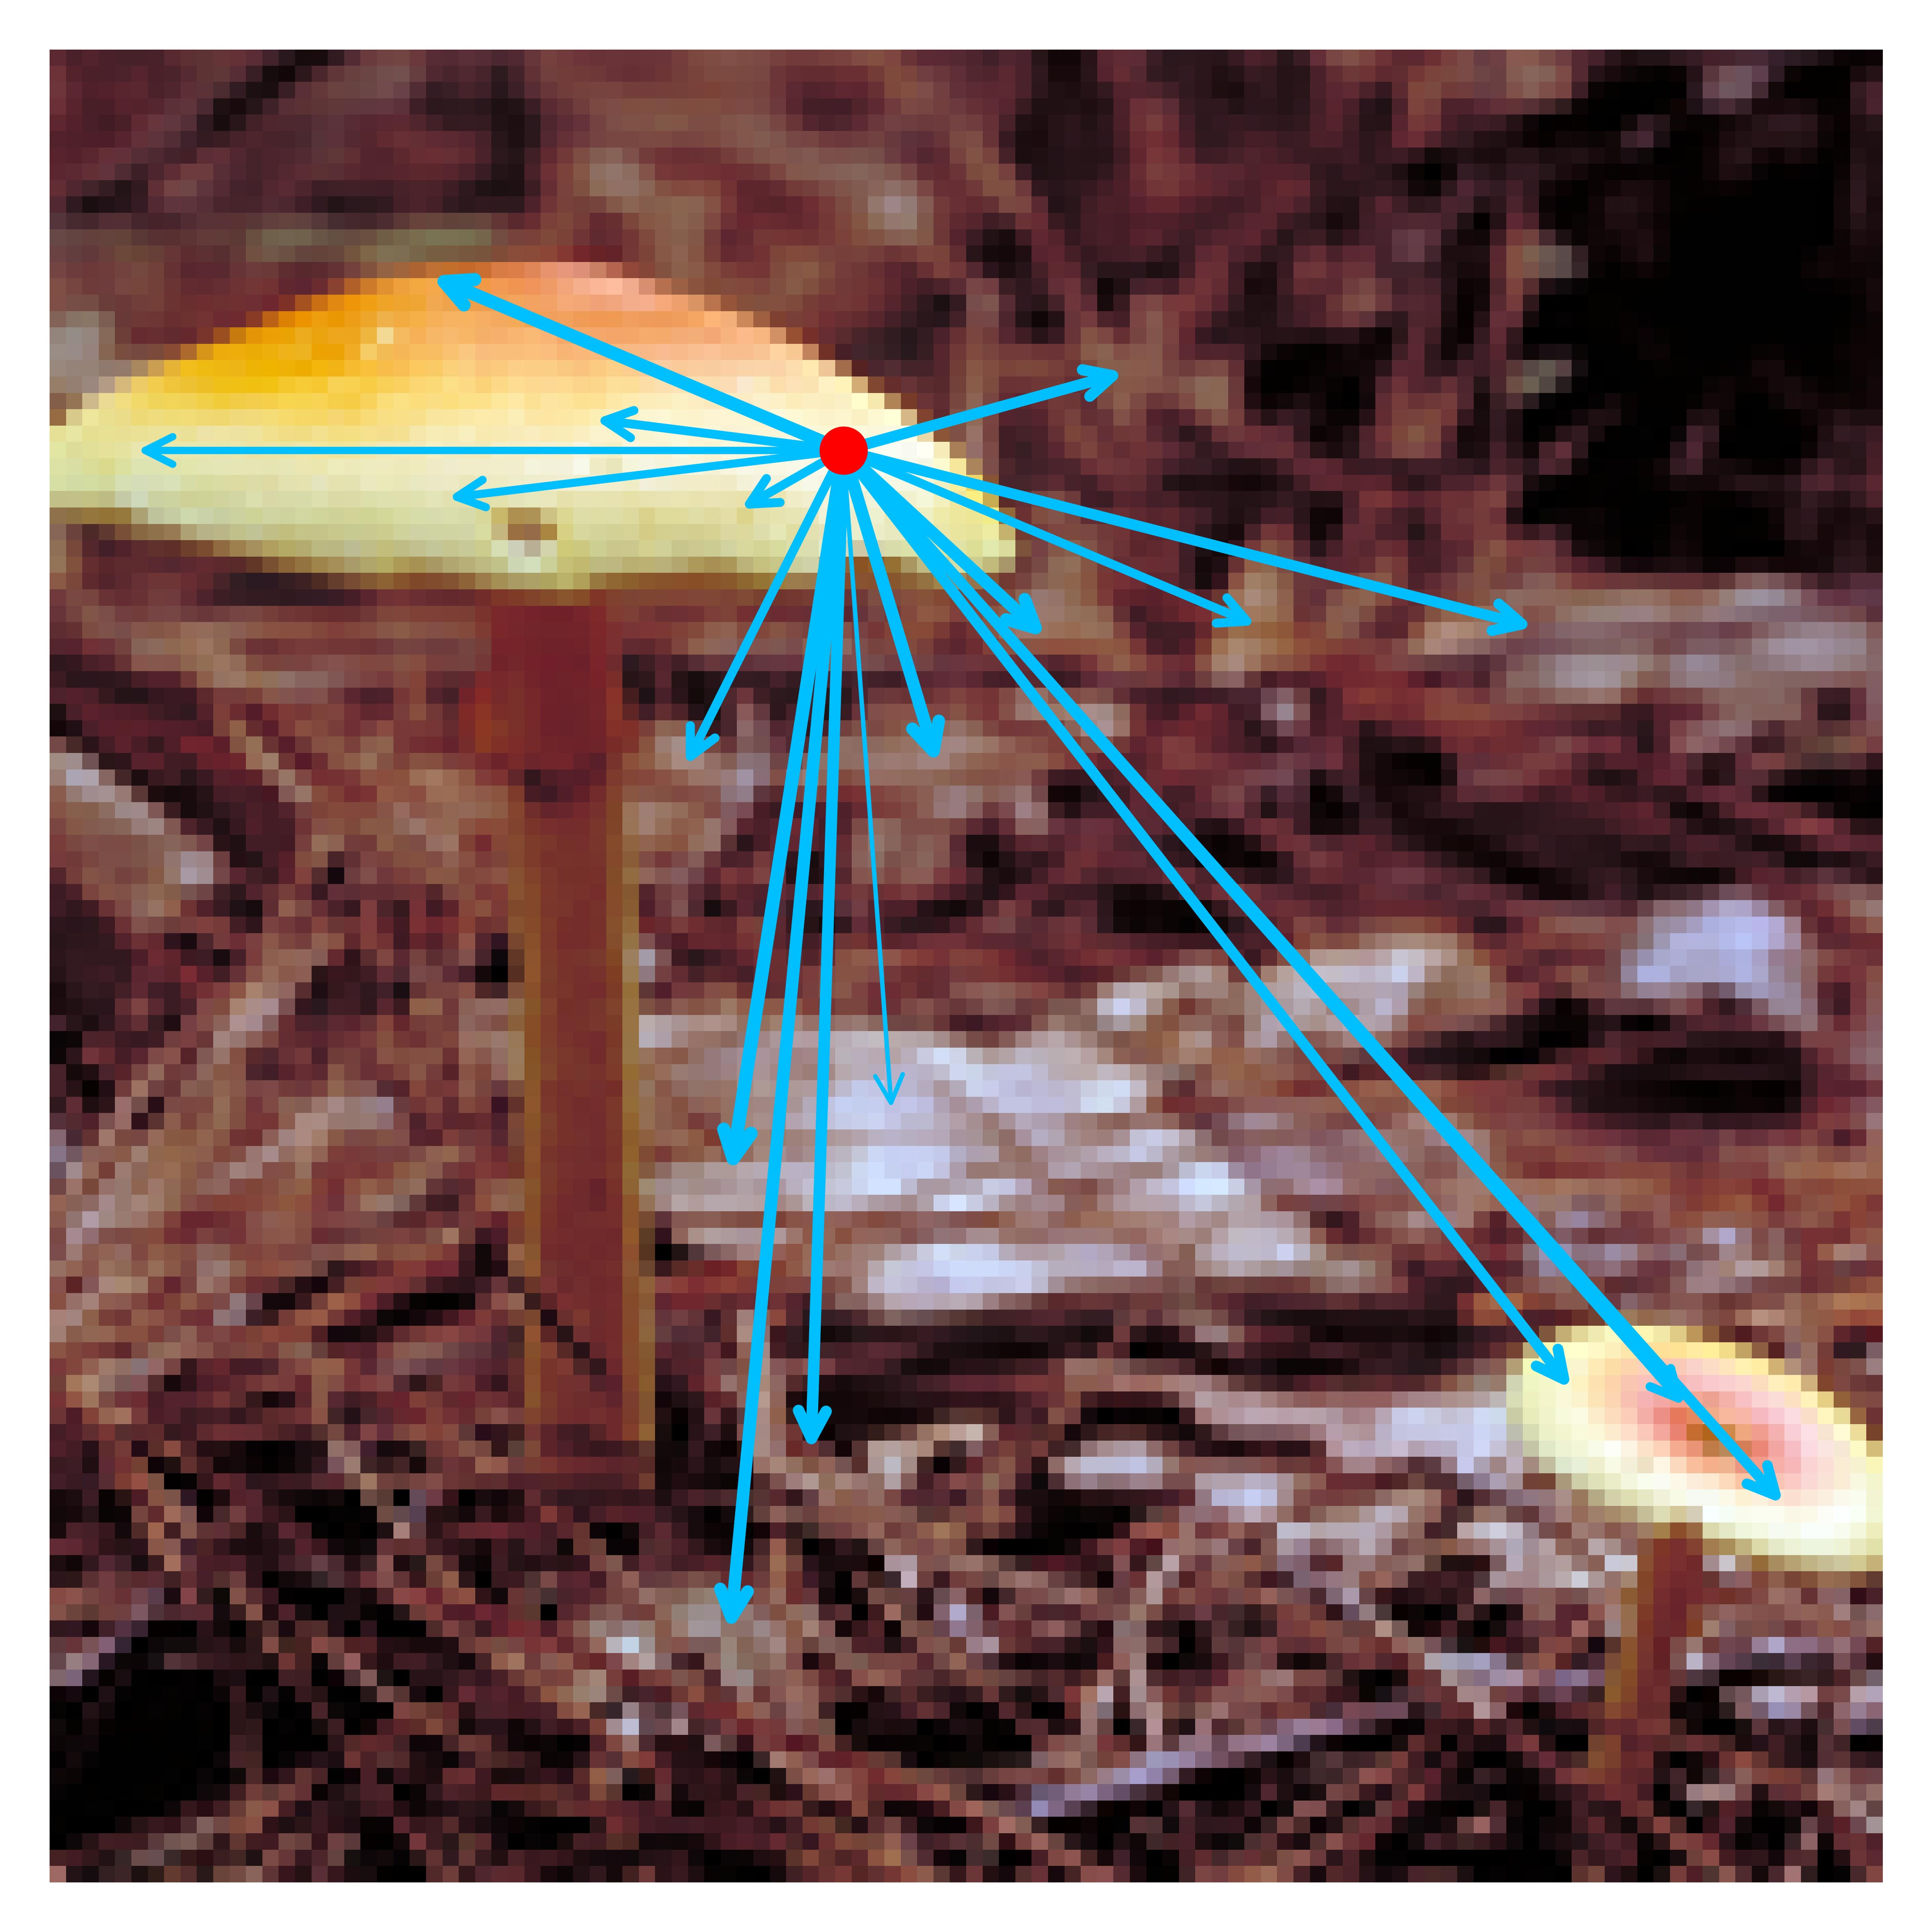
\includegraphics[width=1.9in]{fig/shroom_superpixel.jpg}
			\centerline{(d)}
		\end{minipage}
		\begin{minipage}[t]{.32\linewidth}
			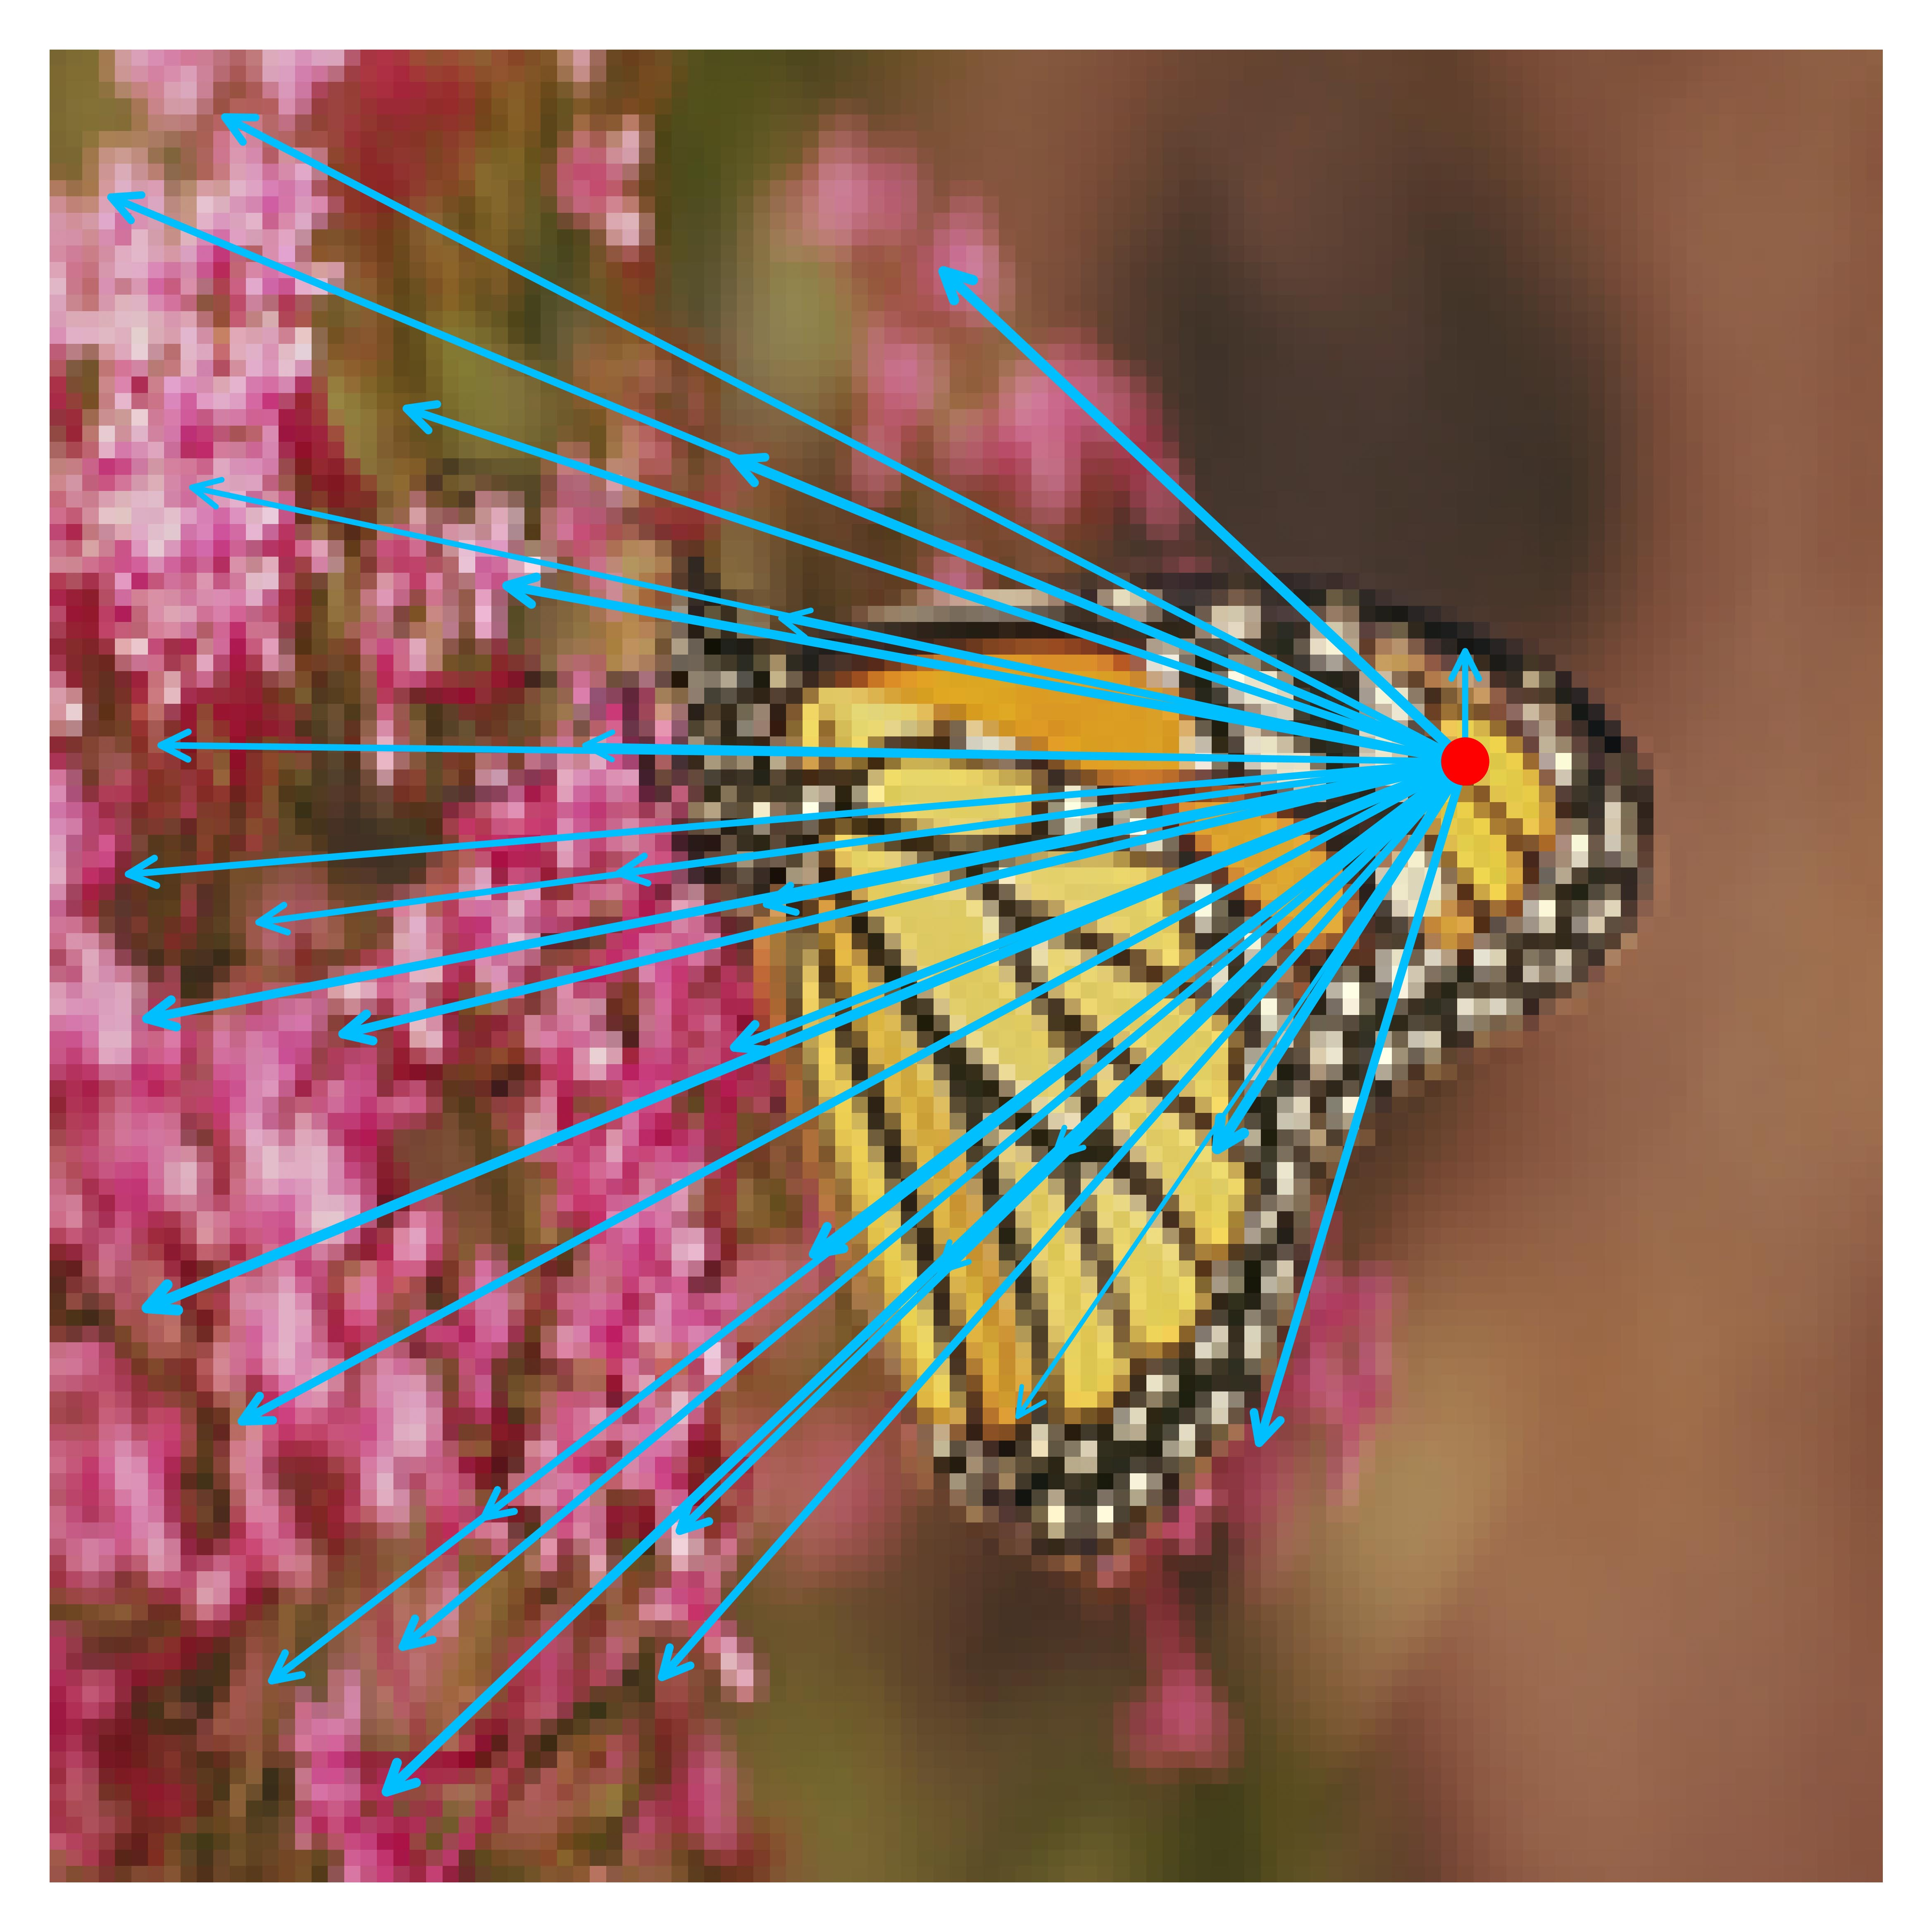
\includegraphics[width=1.9in]{fig/monarch_superpixel.jpg}
			\centerline{(e)}
		\end{minipage}
		\begin{minipage}[t]{.32\linewidth}
			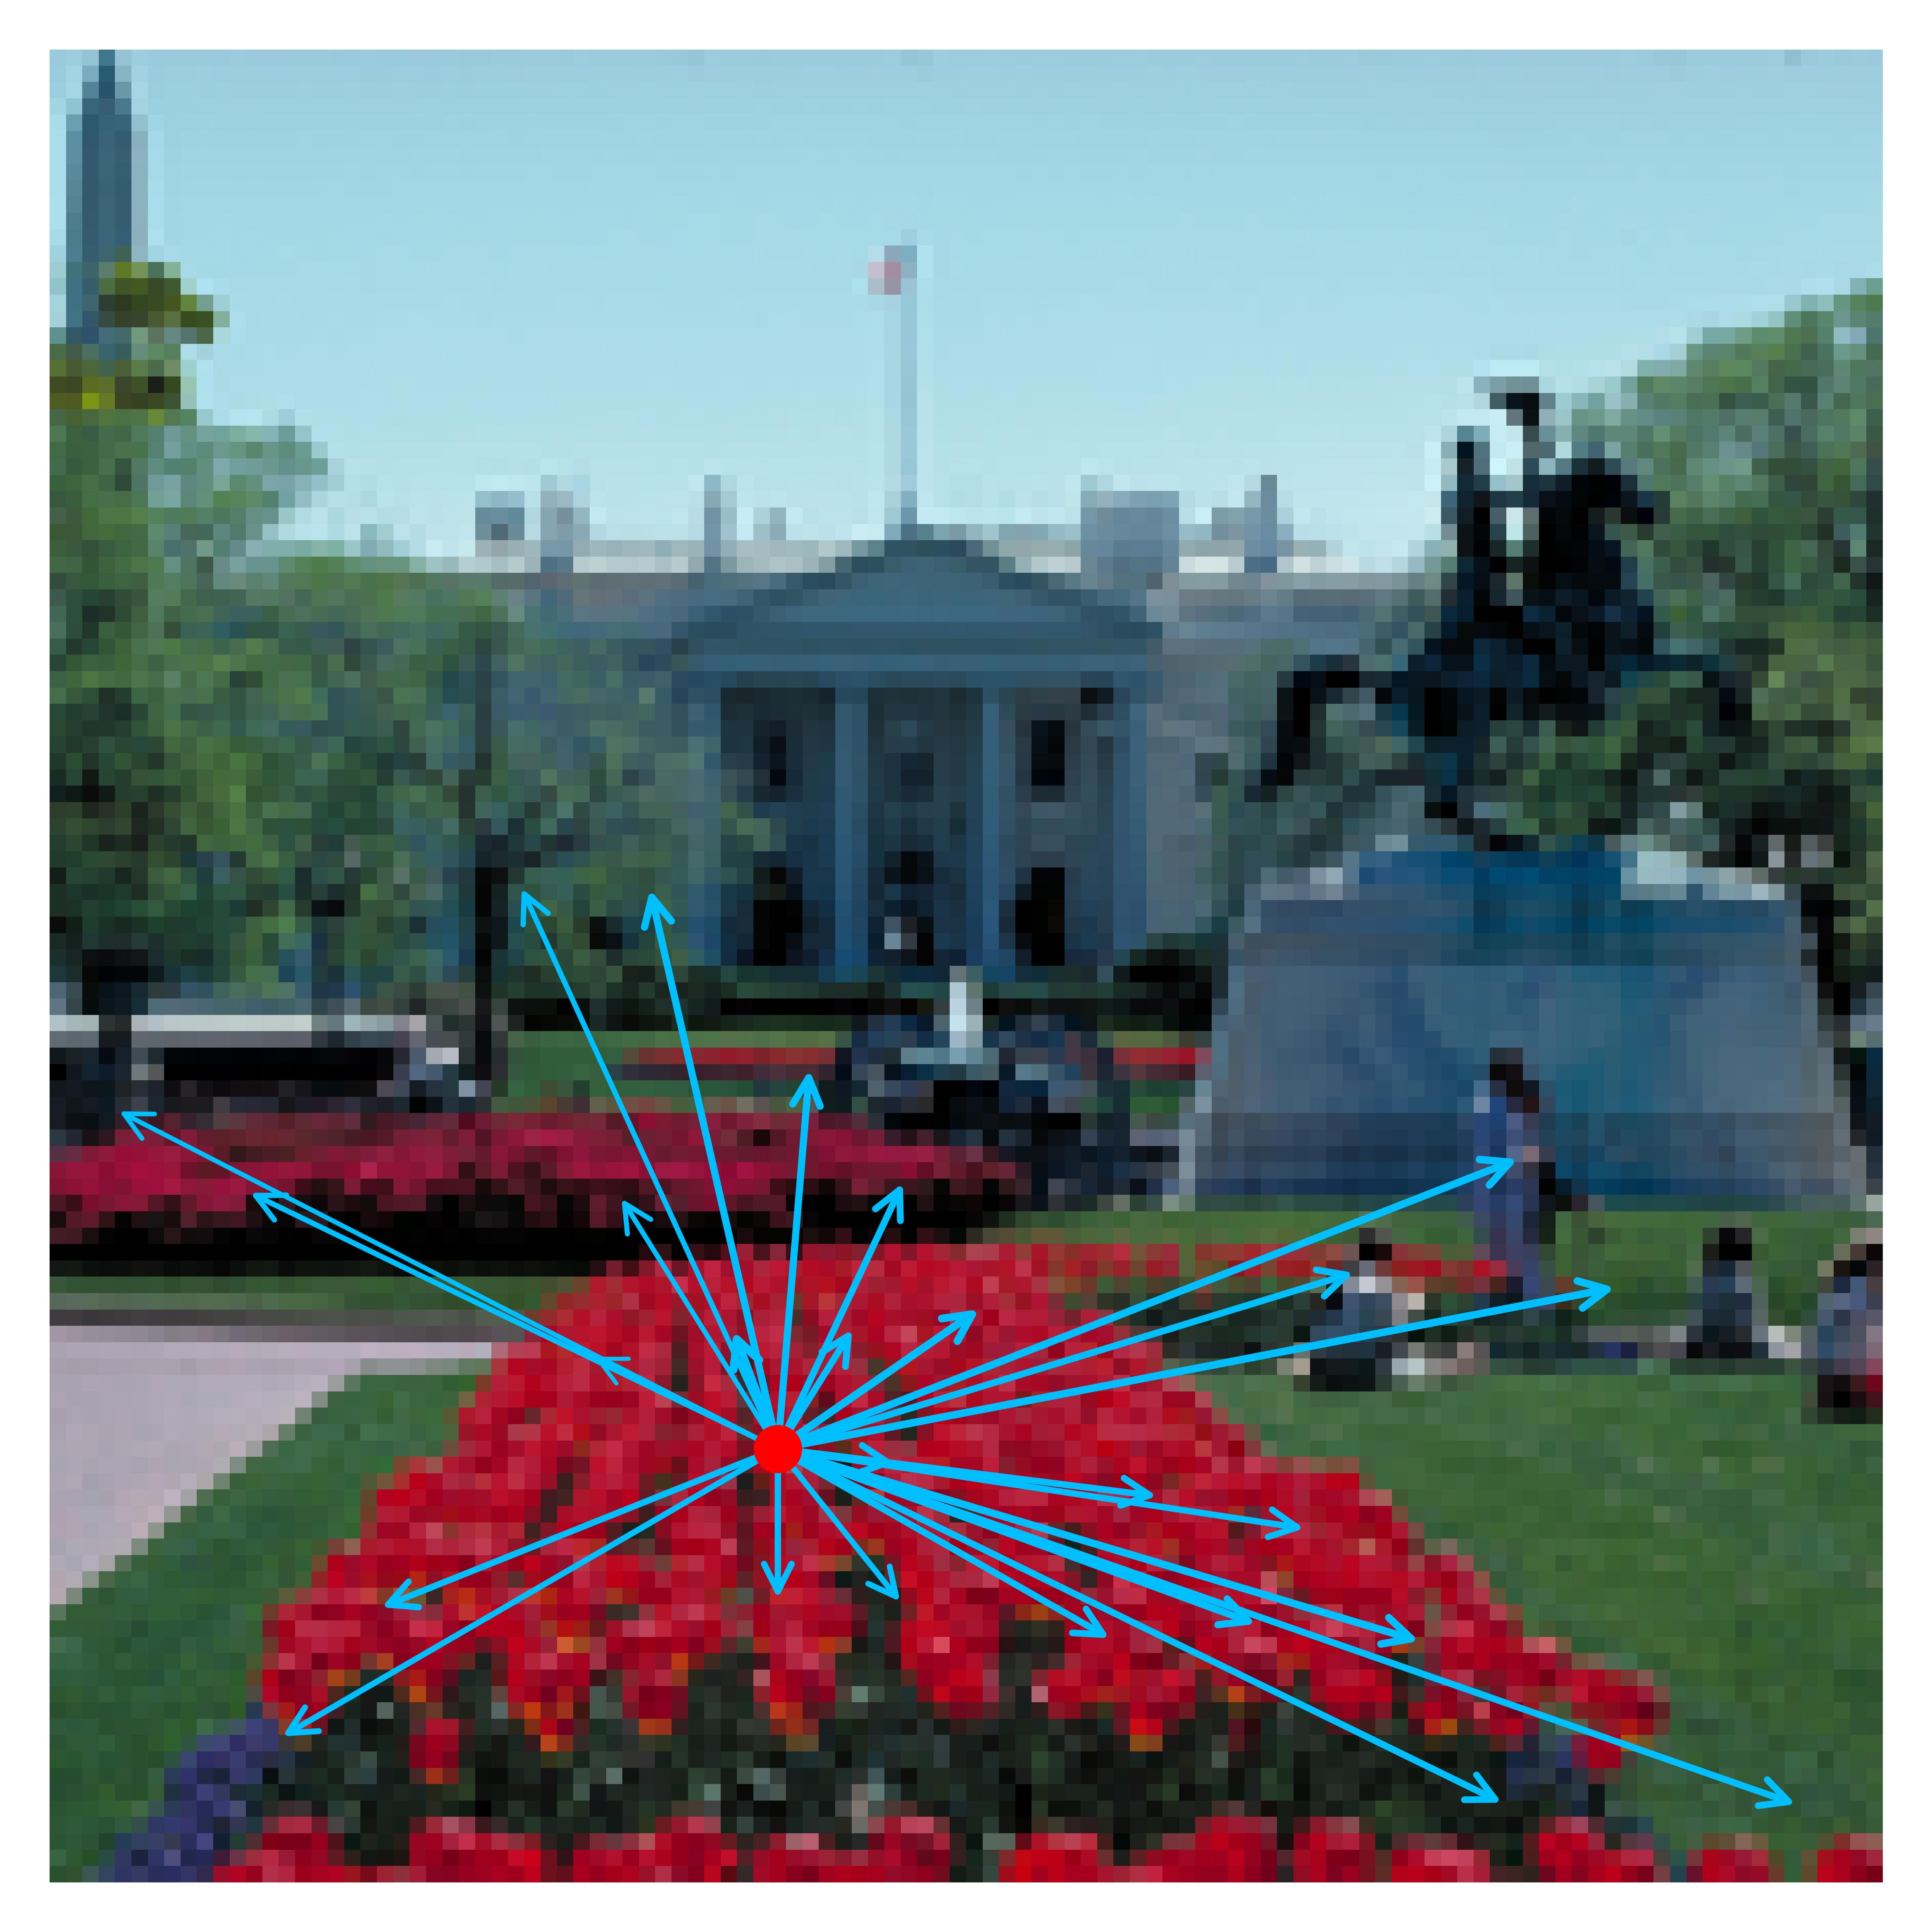
\includegraphics[width=1.9in]{fig/flower_superpixel.jpg}
			\centerline{(f)}
		\end{minipage}
		\caption{The non-local behavior of the long-range dependency and relational modeling. (a) The plane image with a query on wings. (b) The boat image with a query on nearby river bank. (c) The Statue of Liberty image with a query on the lady. (d) The shrooms image with a query on one shroom. (e) The butterfly image with a query on the wing. (f) The Lafayette Square, Washington, D.C.~image with a query on flowers.}
		\label{Non-local Behavior from the TID2013 database}
	\end{figure}
	In the plane image (\reffig{Non-local Behavior from the TID2013 database}~(a)), when the query is in the aircraft wings, the learned corresponding dependencies are mainly centralized to the jet's fuselage. In the boat image (\reffig{Non-local Behavior from the TID2013 database}~(b)), the river banks are closely correlated with the boat floating in the water. In the Statue of Liberty image (\reffig{Non-local Behavior from the TID2013 database}~(c)), a part of the lady's body is tightly connected with other parts. In the shrooms image (\reffig{Non-local Behavior from the TID2013 database}~(d)), one shroom is bound up with itself and the other shrooms. In the butterfly image (\reffig{Non-local Behavior from the TID2013 database}~(e)), the butterfly's wings correlate with the butterfly itself and have relations with the surrounding flowers. Lastly, in the Lafayette Square, Washington, D.C.~image (\reffig{Non-local Behavior from the TID2013 database}~(f)), the flowers are closely related to other flowers and the feasting crowd. From these demonstrations, the long-range dependencies and relationships among objects in the image are encoded from the non-local interactions among different image regions.
	\begin{figure*}[]
		\centering
		\begin{minipage}[t]{.24\linewidth}
			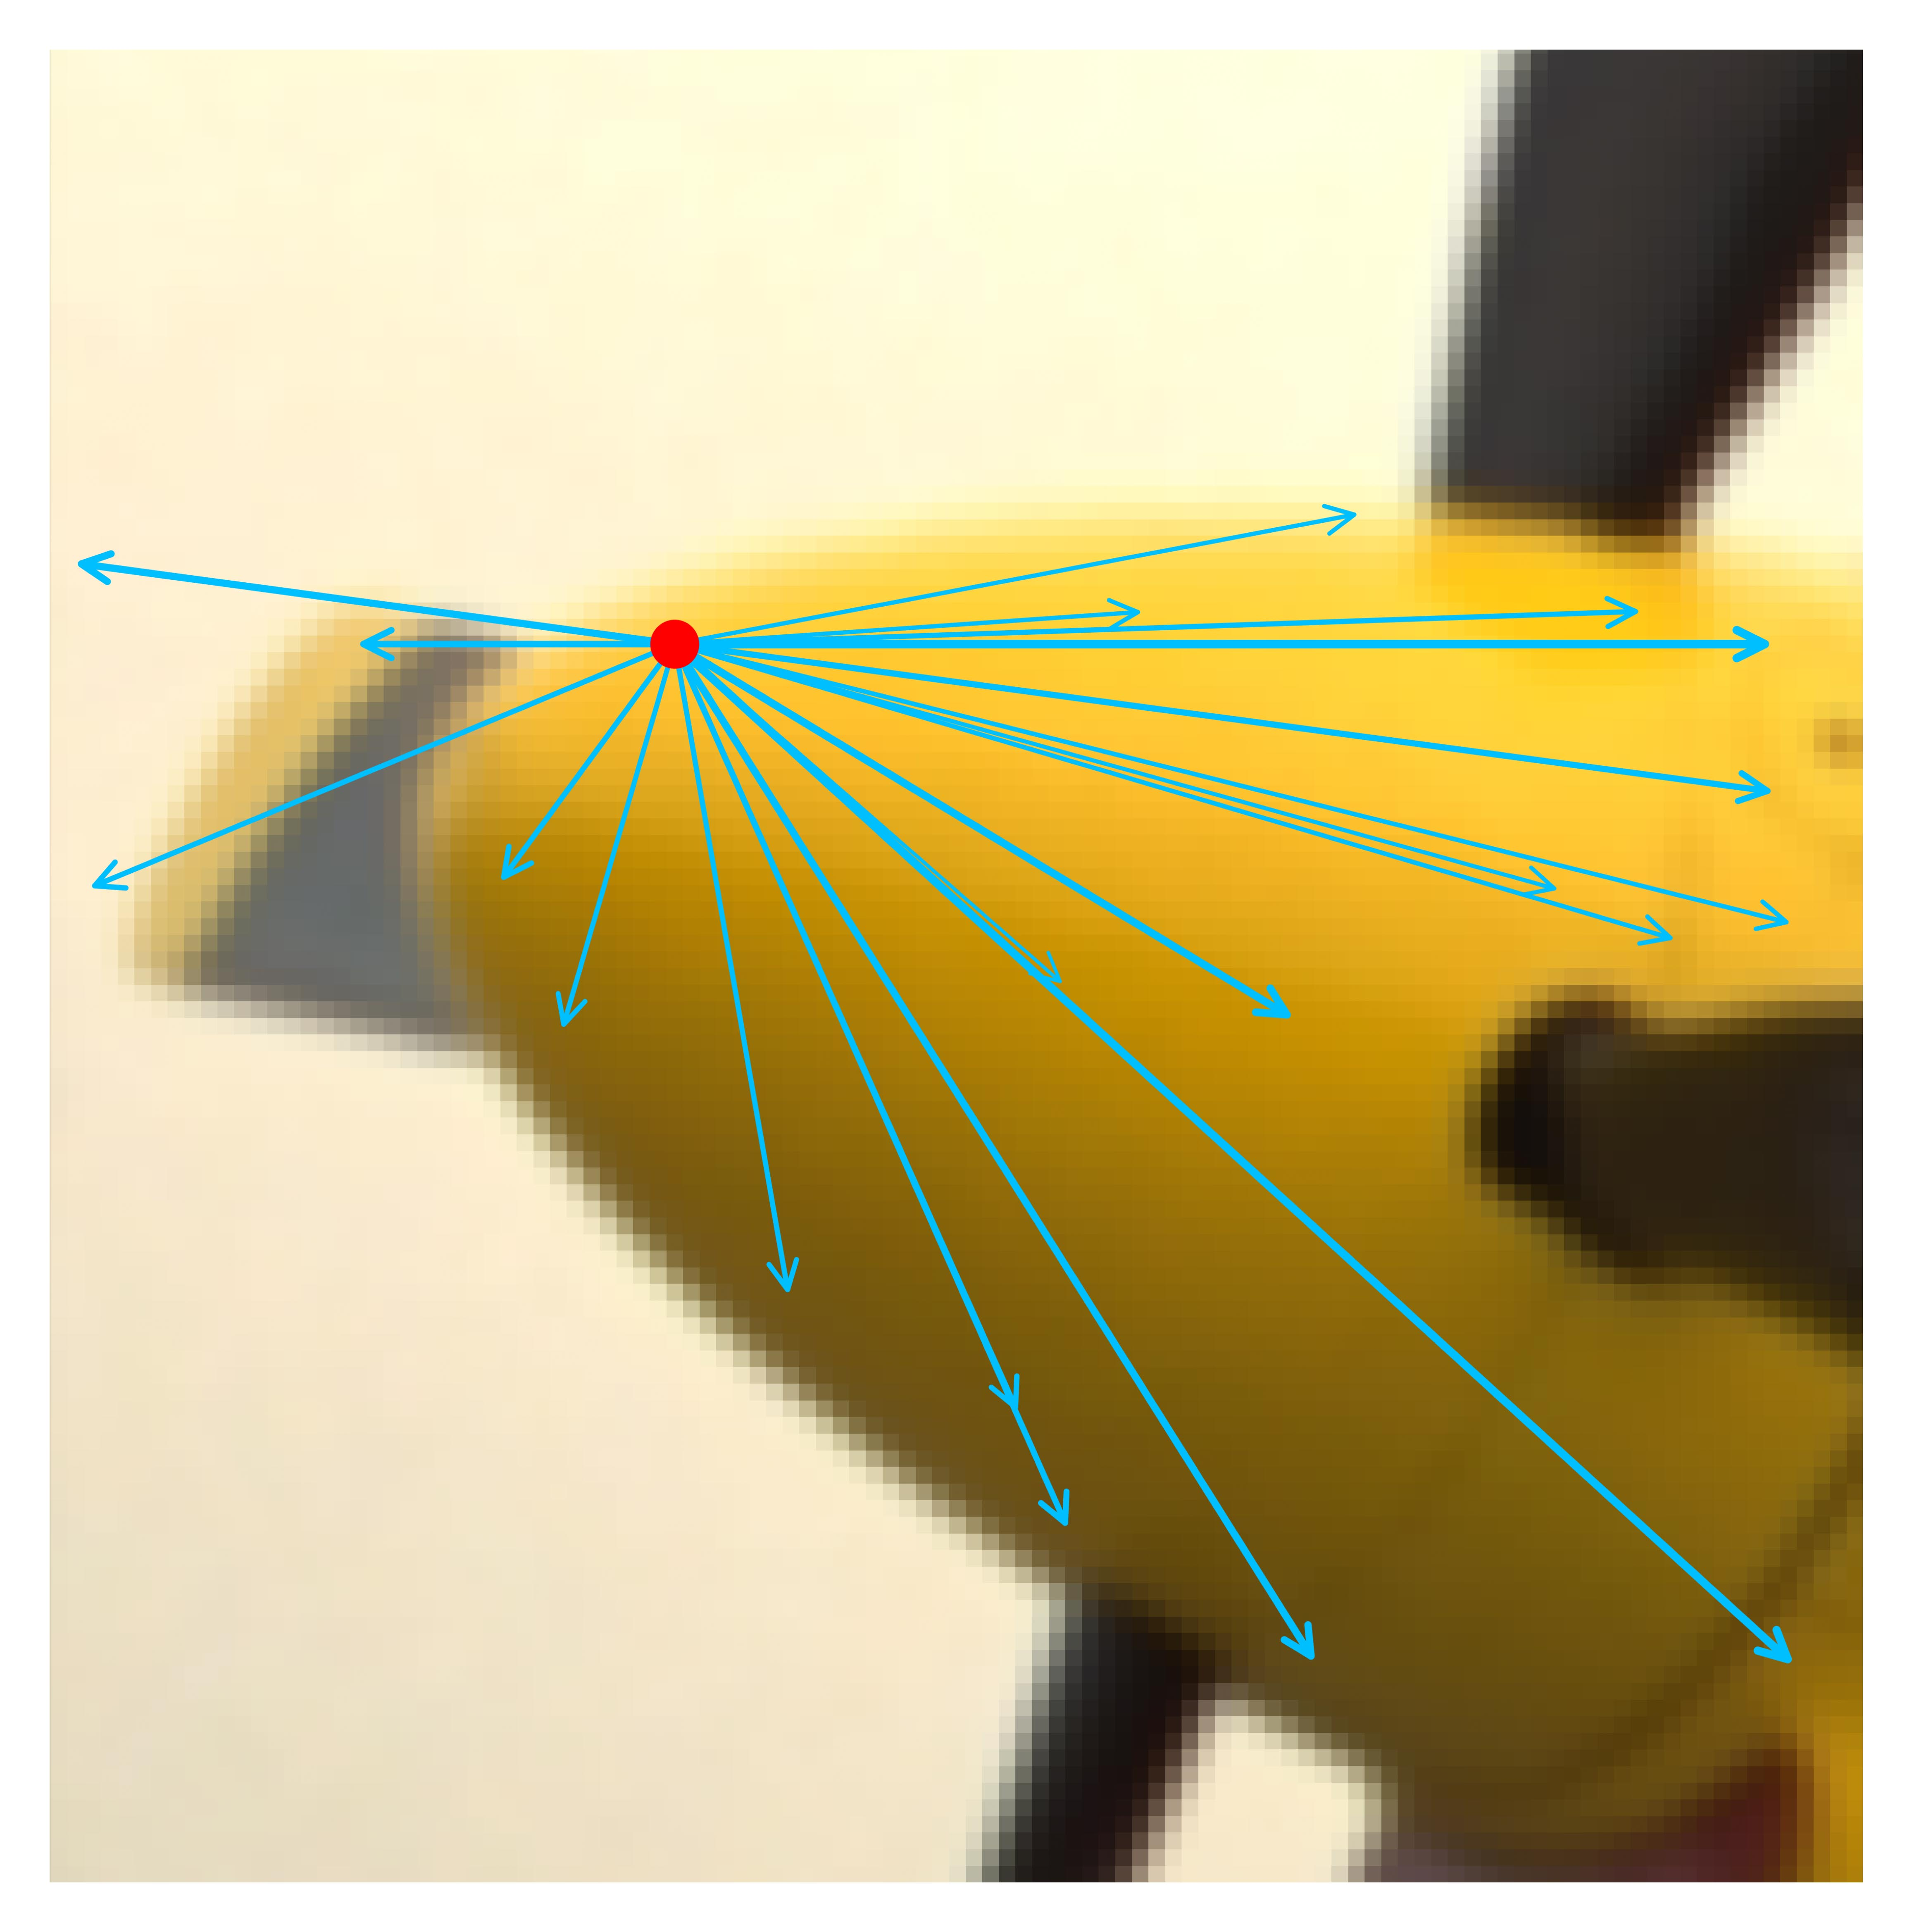
\includegraphics[width=1.5in]{cropped/jet_superpixel_4.jpg}
			\centerline{(a)}
			\label{JET-1}
		\end{minipage}
		\begin{minipage}[t]{.24\linewidth}
			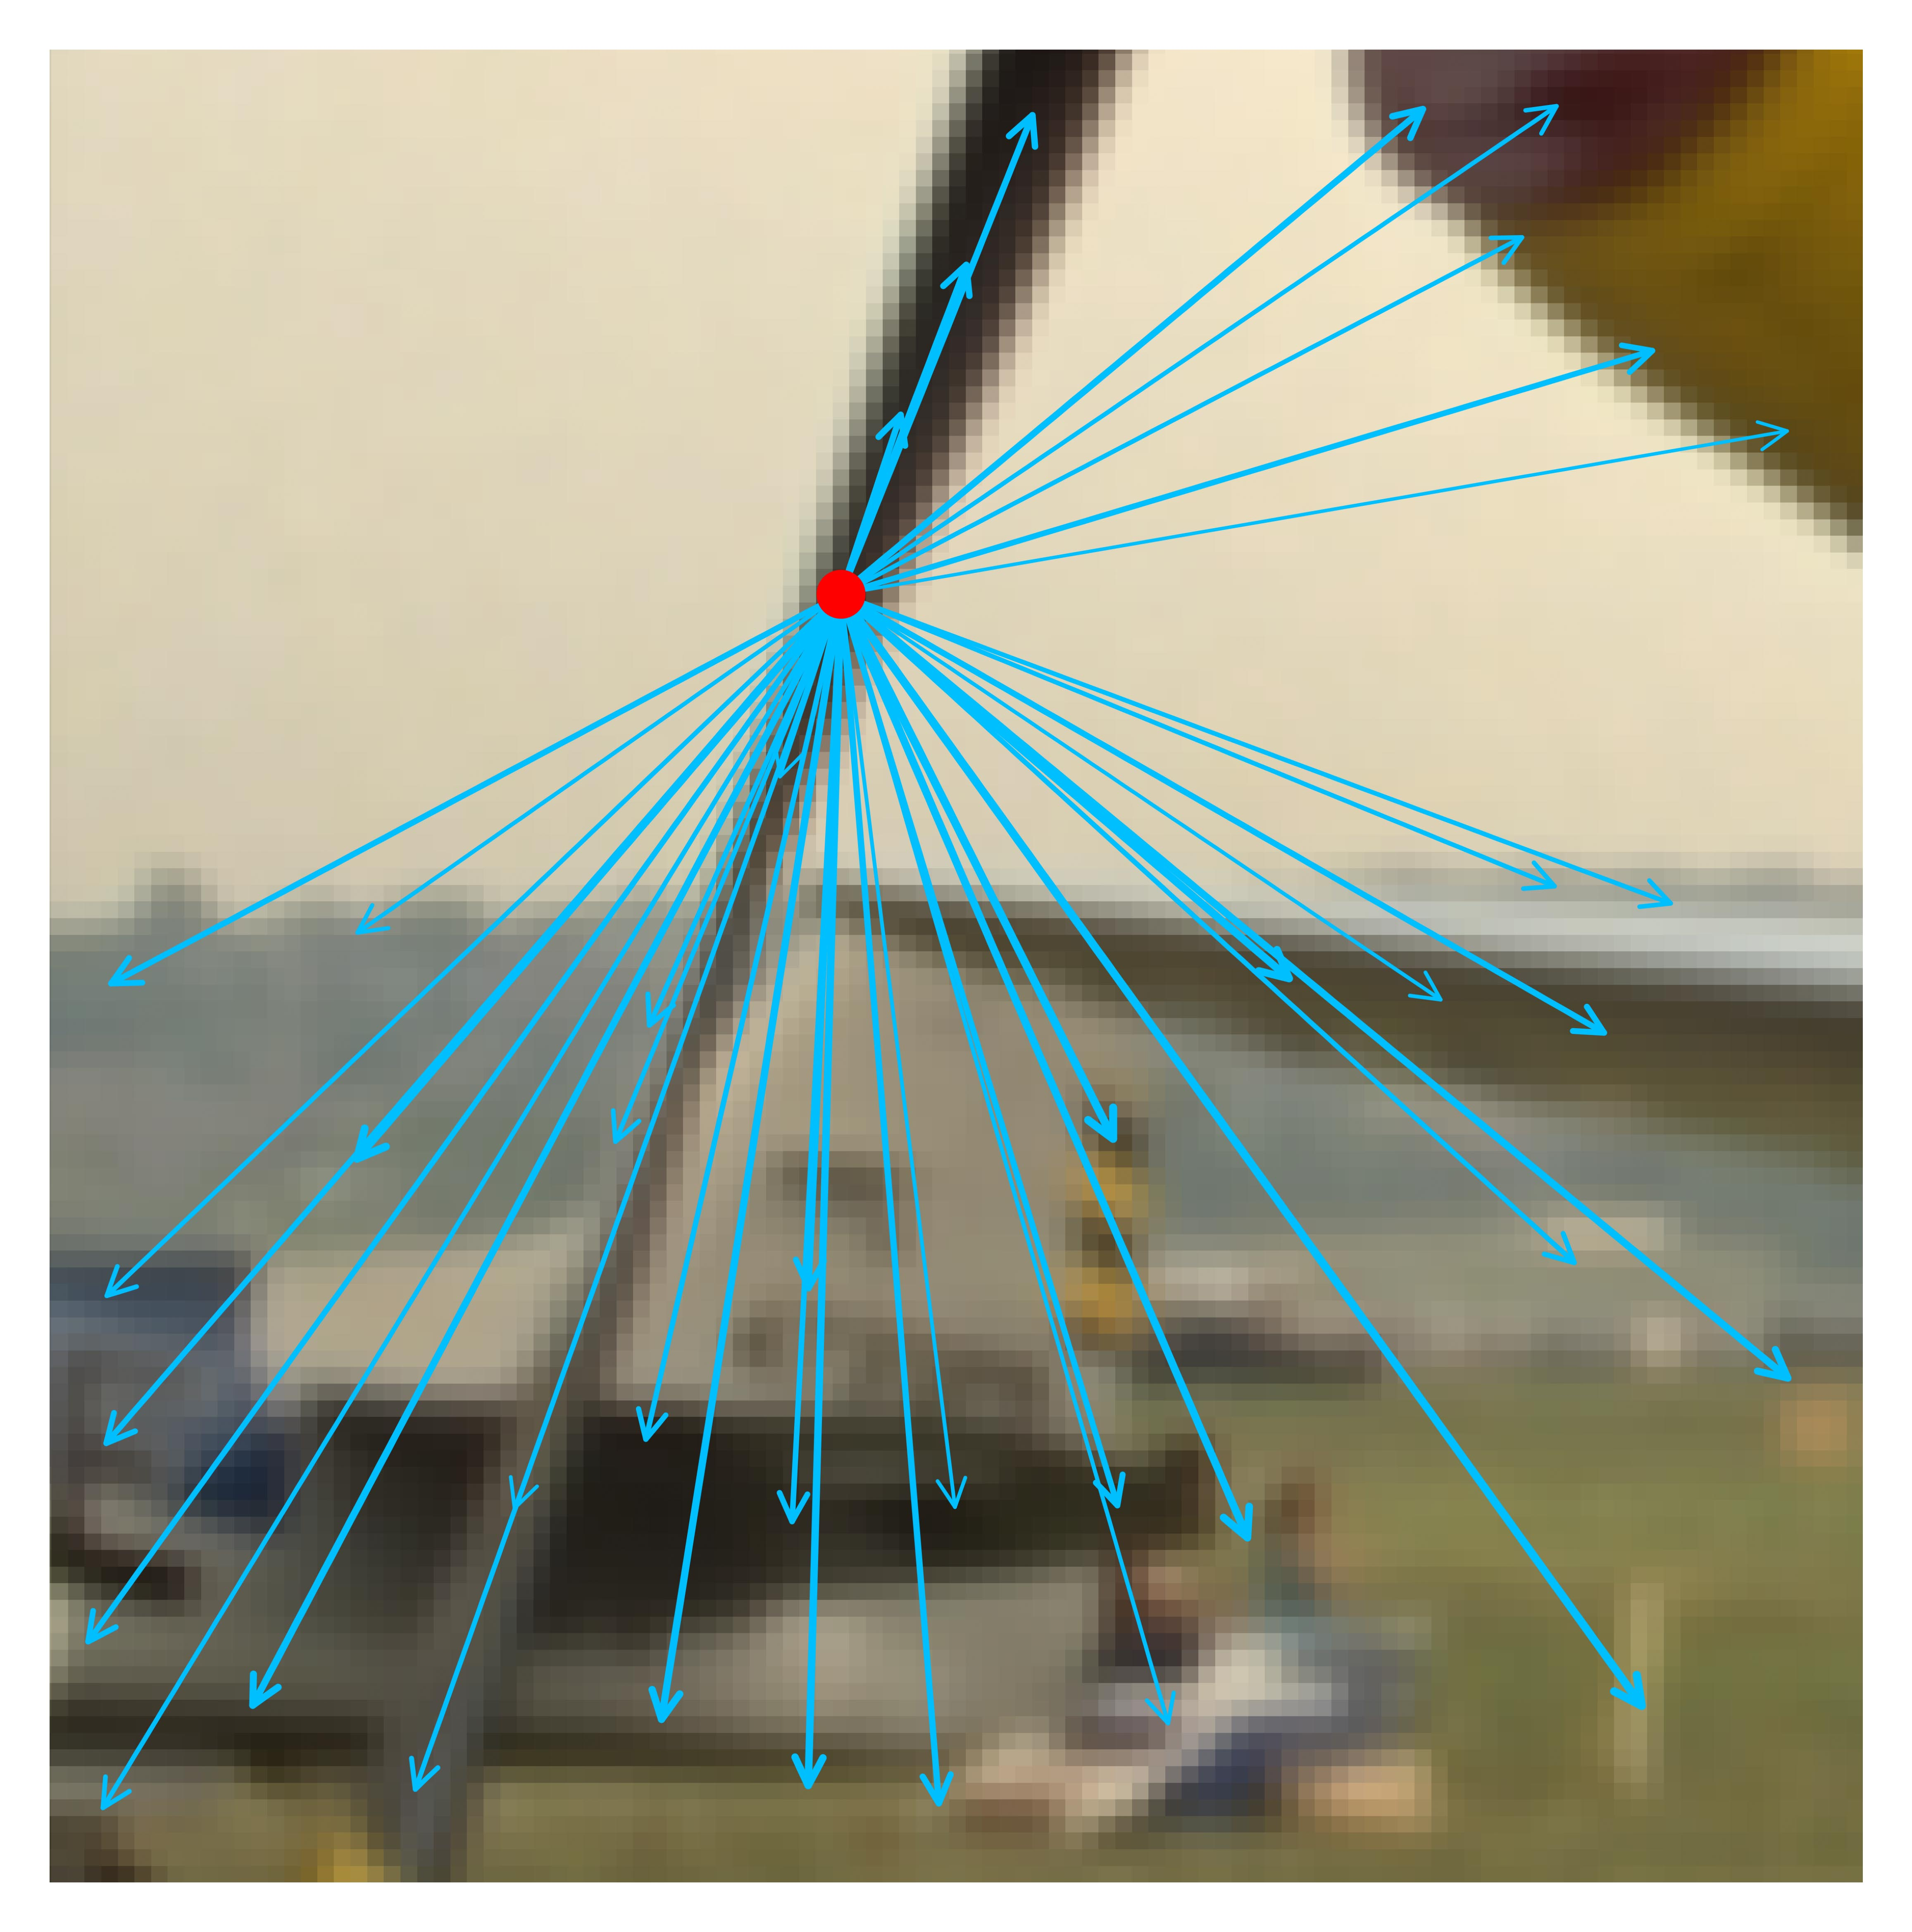
\includegraphics[width=1.5in]{cropped/jet_superpixel_8.jpg}
			\centerline{(b)}
			\label{JET-2}
		\end{minipage}
		\begin{minipage}[t]{.24\linewidth}
			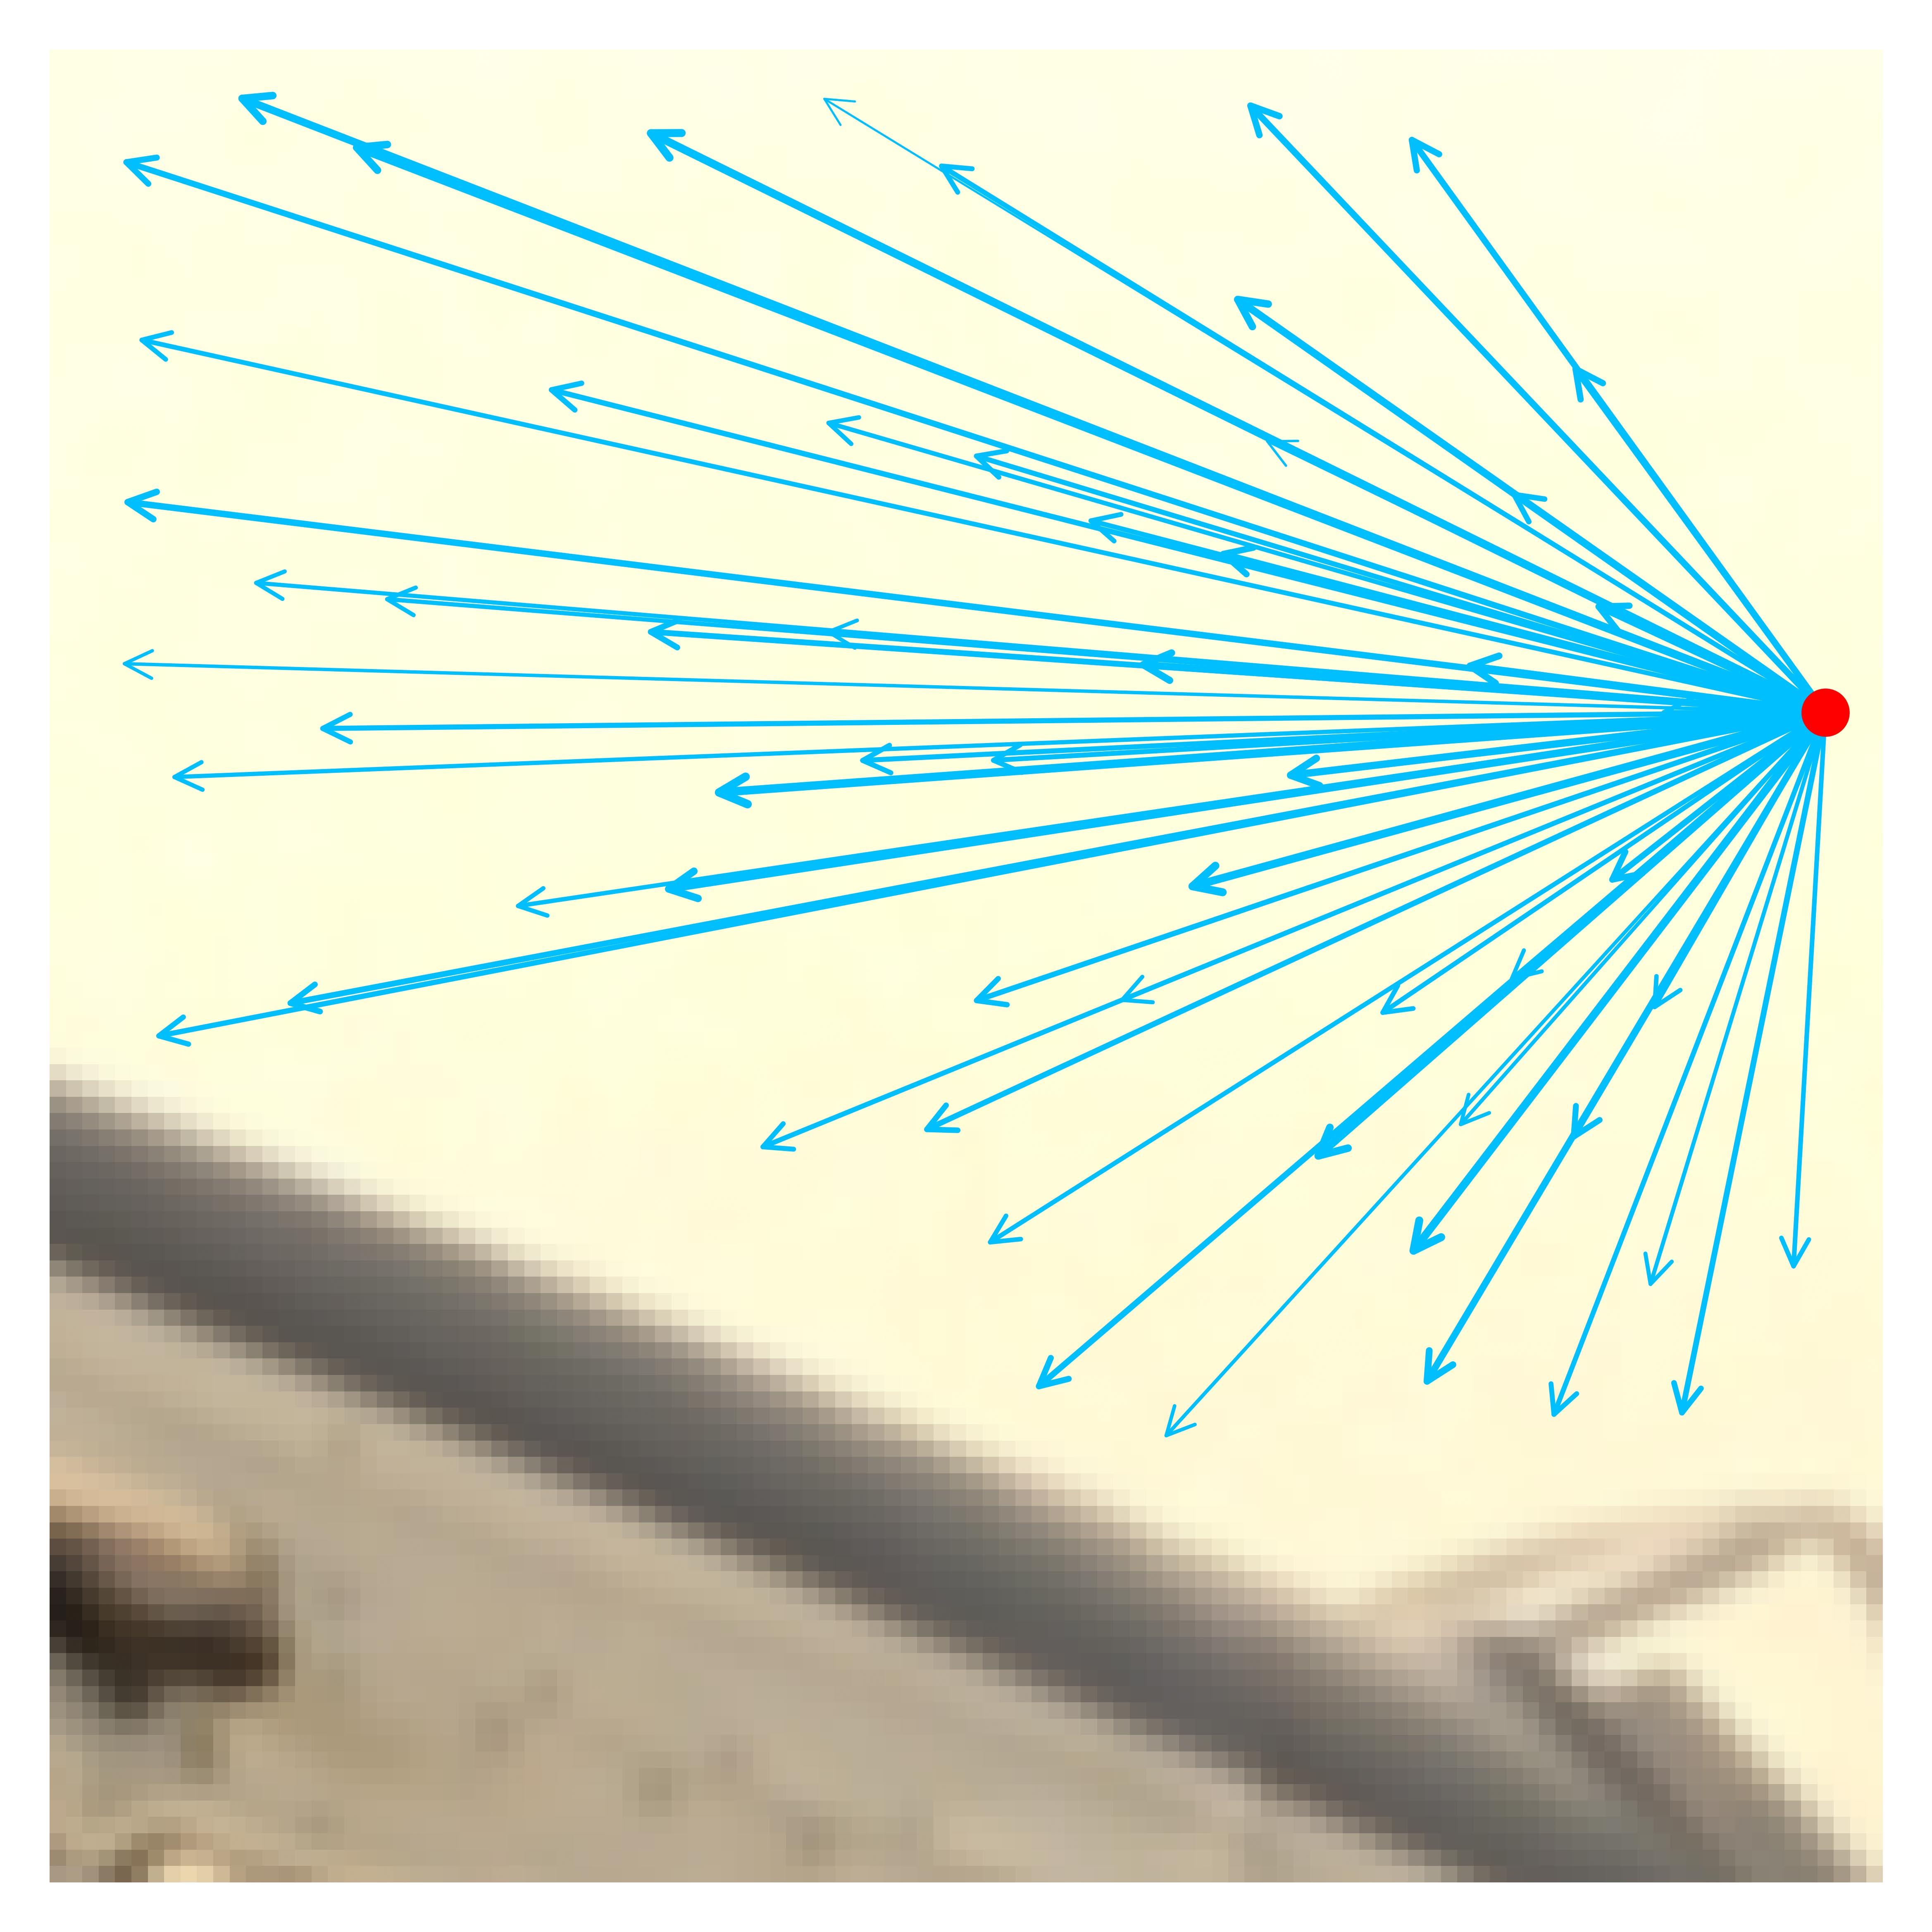
\includegraphics[width=1.5in]{cropped/jet_superpixel_6.jpg}
			\centerline{(c)}
			\label{JET-3}
		\end{minipage}
		\begin{minipage}[t]{.24\linewidth}
			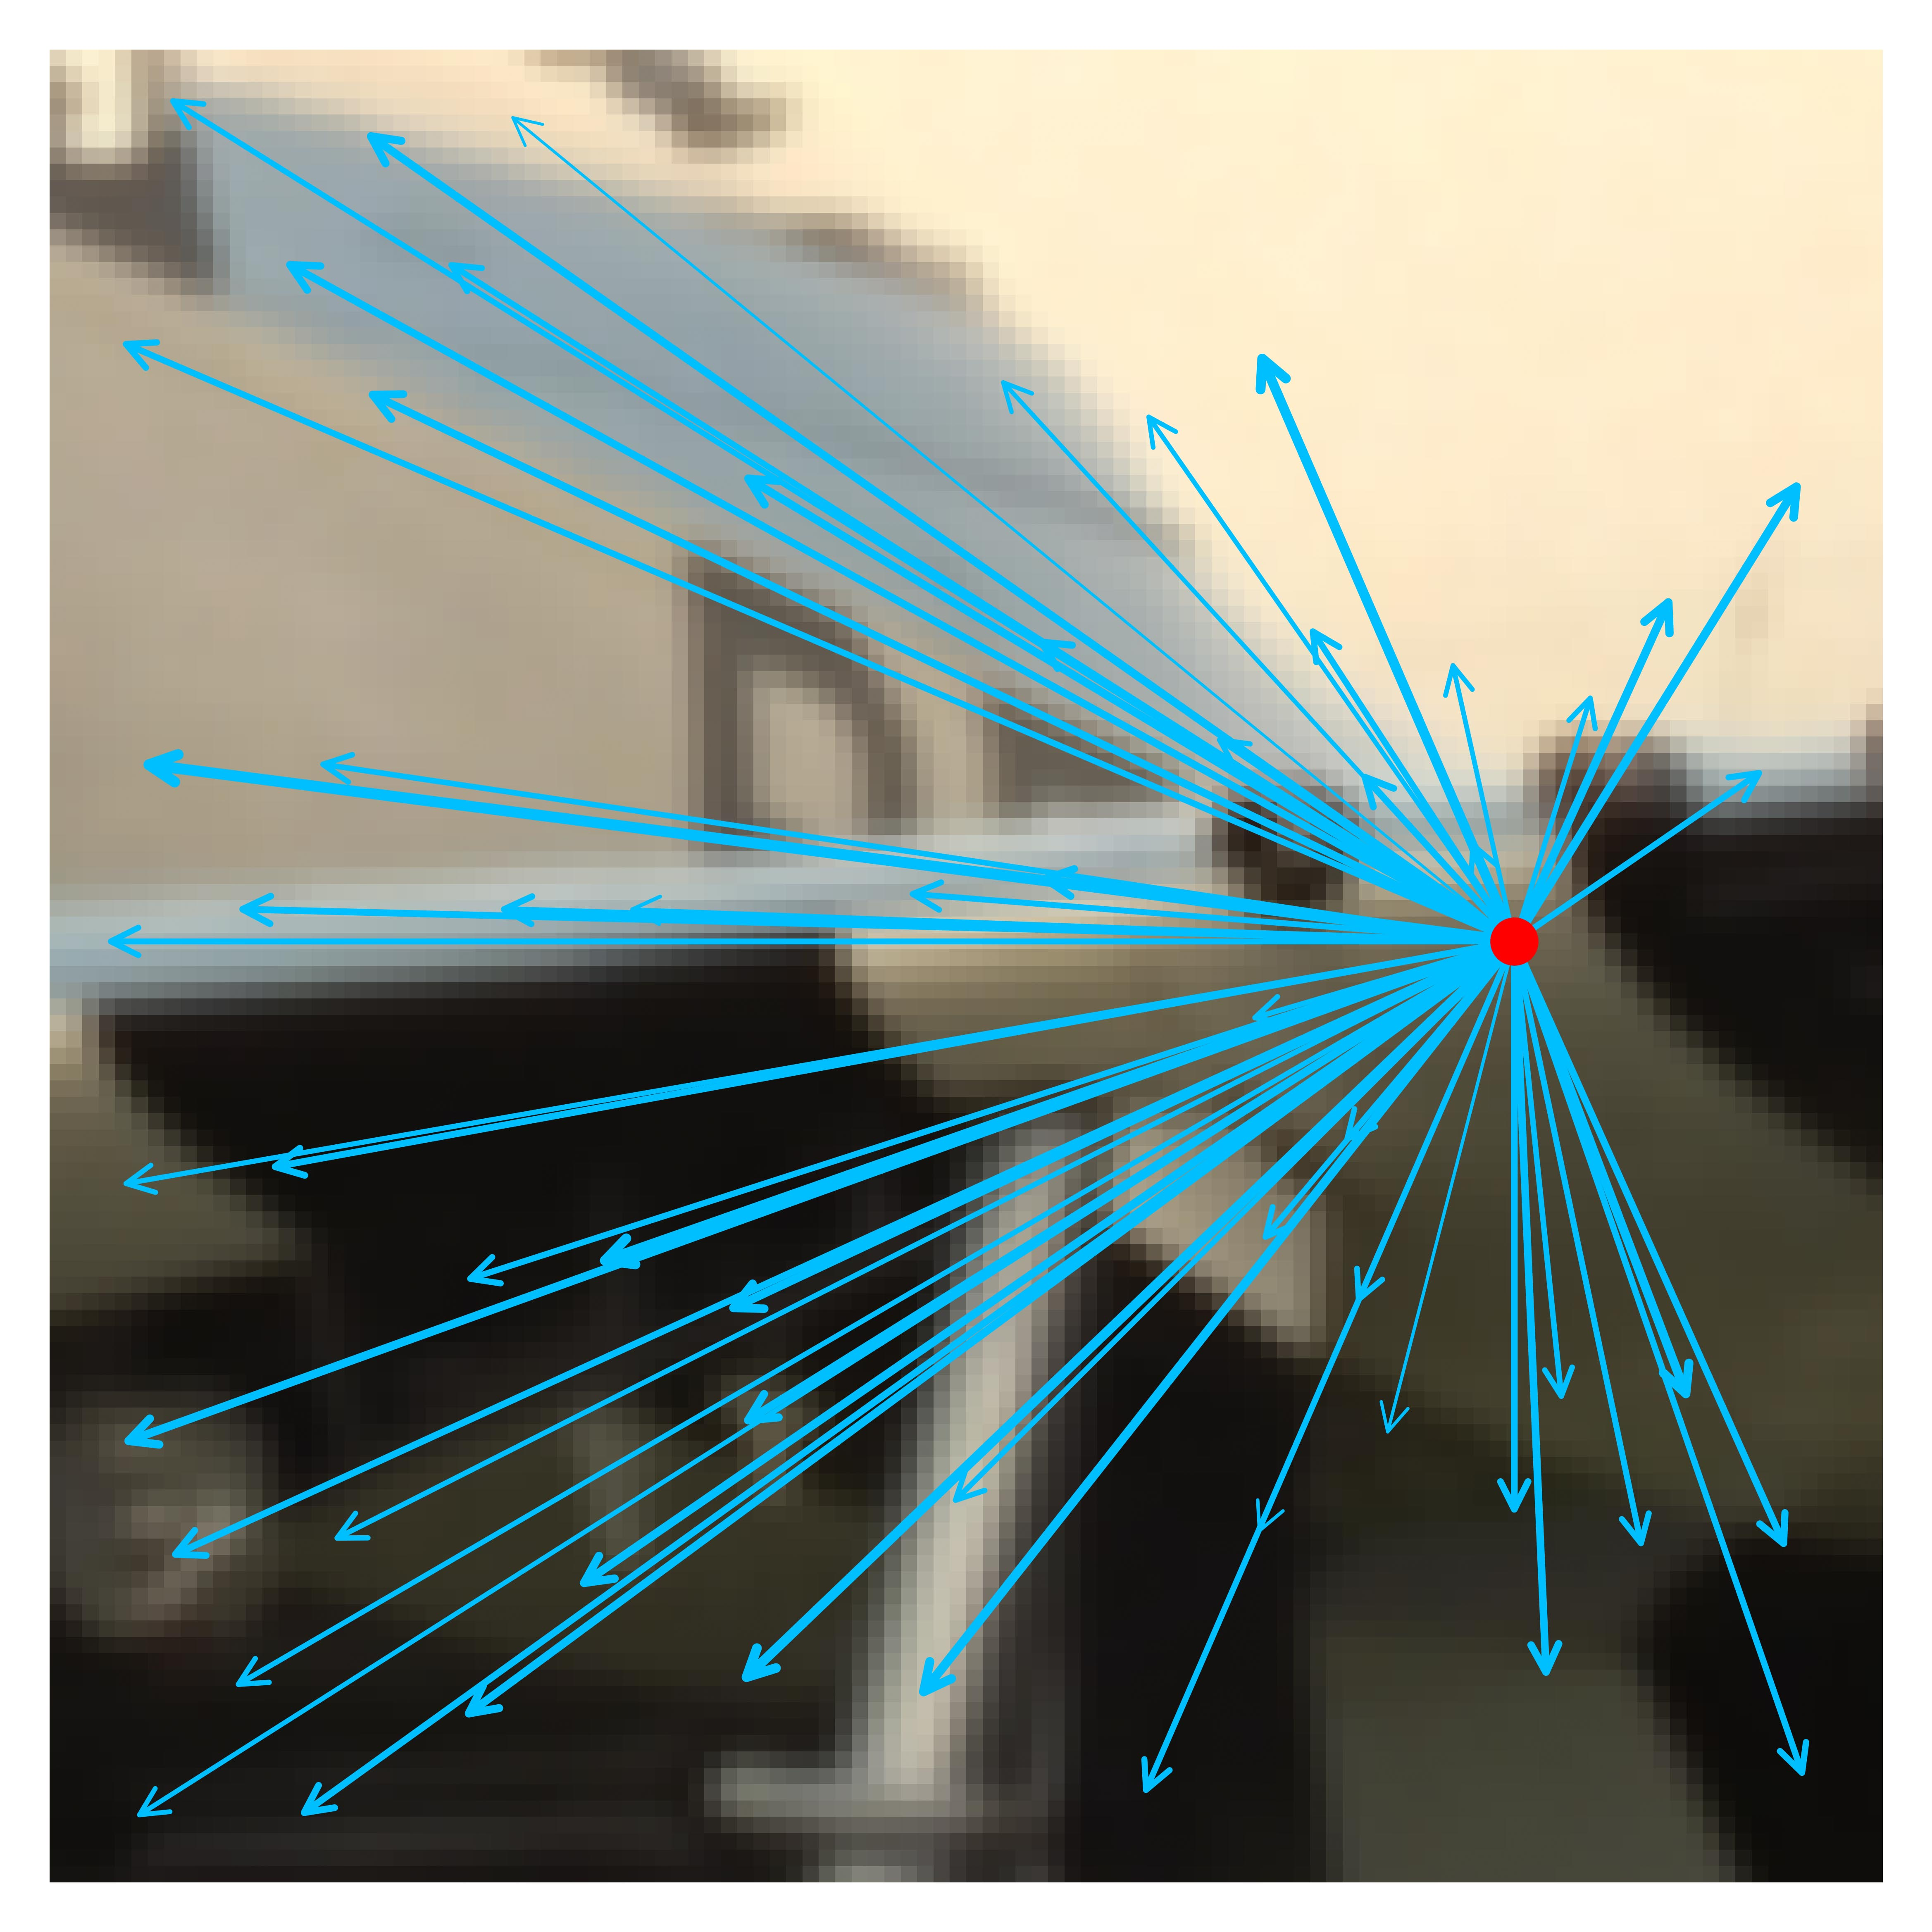
\includegraphics[width=1.5in]{cropped/jet_superpixel_11.jpg}
			\centerline{(d)}
			\label{JET-4}
		\end{minipage}
		\begin{minipage}[t]{.24\linewidth}
			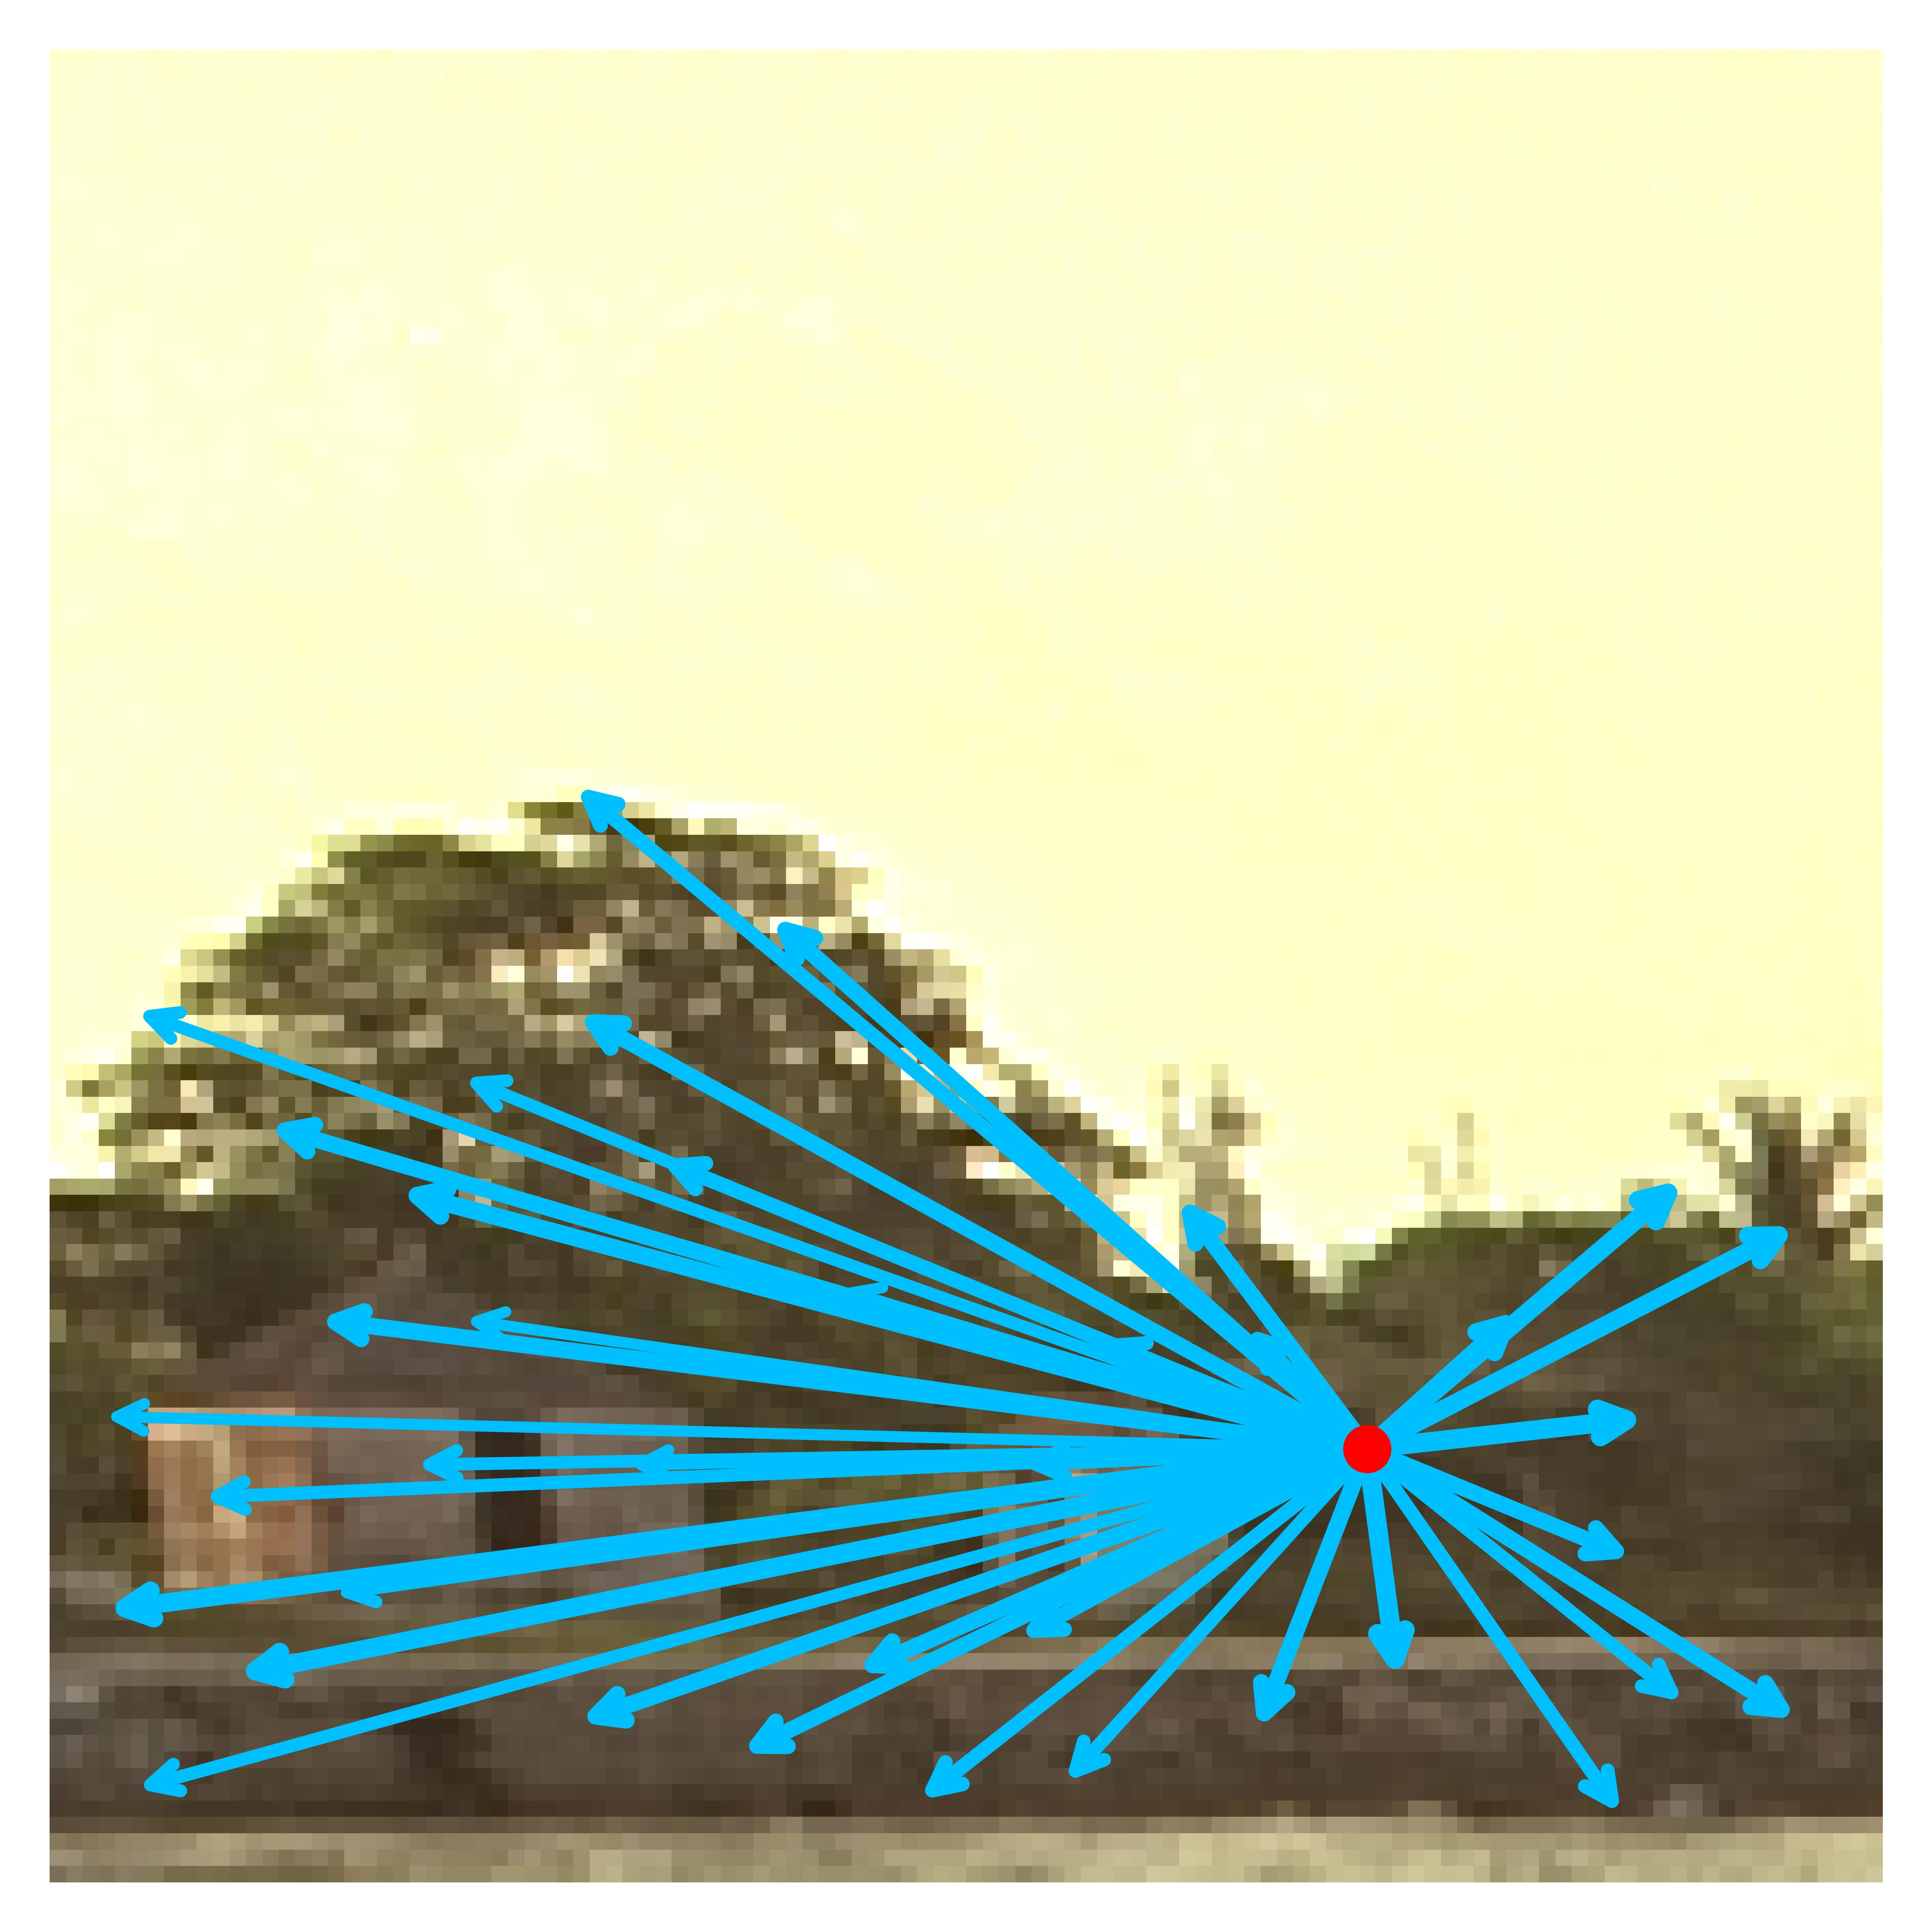
\includegraphics[width=1.5in]{cropped/boat_superpixel_0.jpg}
			\centerline{(e)}
			\label{BOAT-1}
		\end{minipage}
		\begin{minipage}[t]{.24\linewidth}
			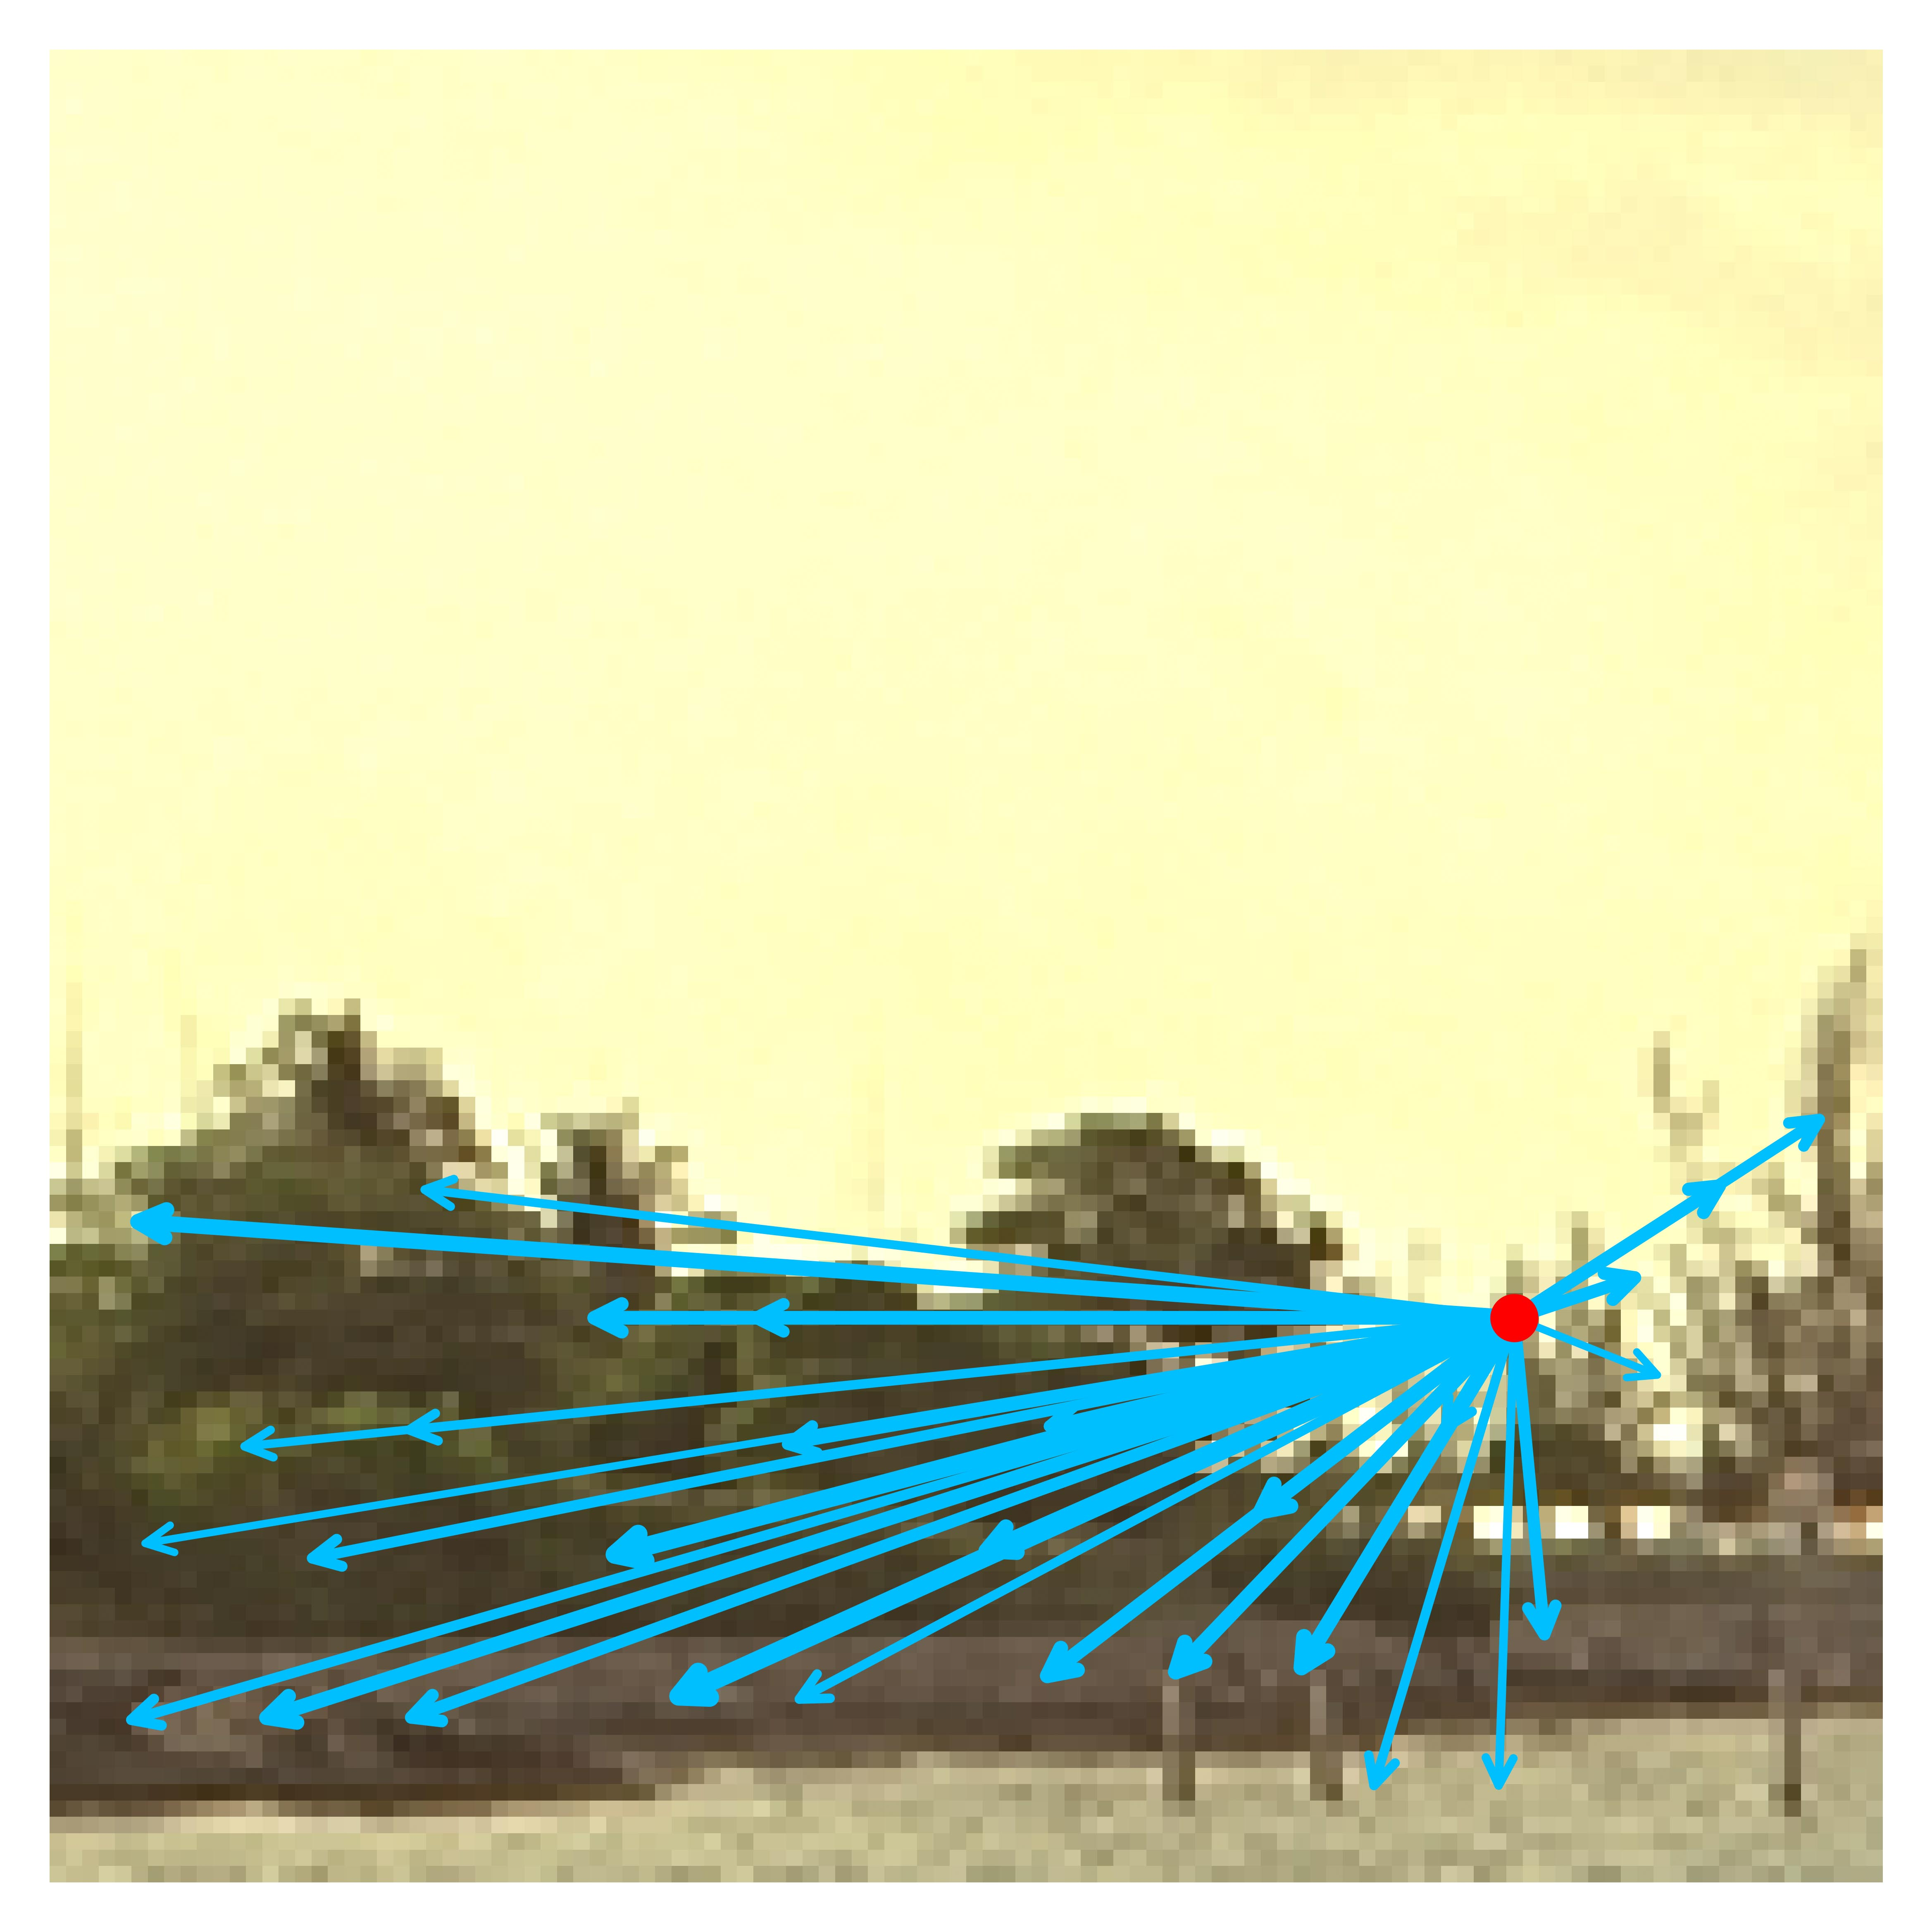
\includegraphics[width=1.5in]{cropped/boat_superpixel_1.jpg}
			\centerline{(f)}
			\label{BOAT-2}
		\end{minipage}
		\begin{minipage}[t]{.24\linewidth}
			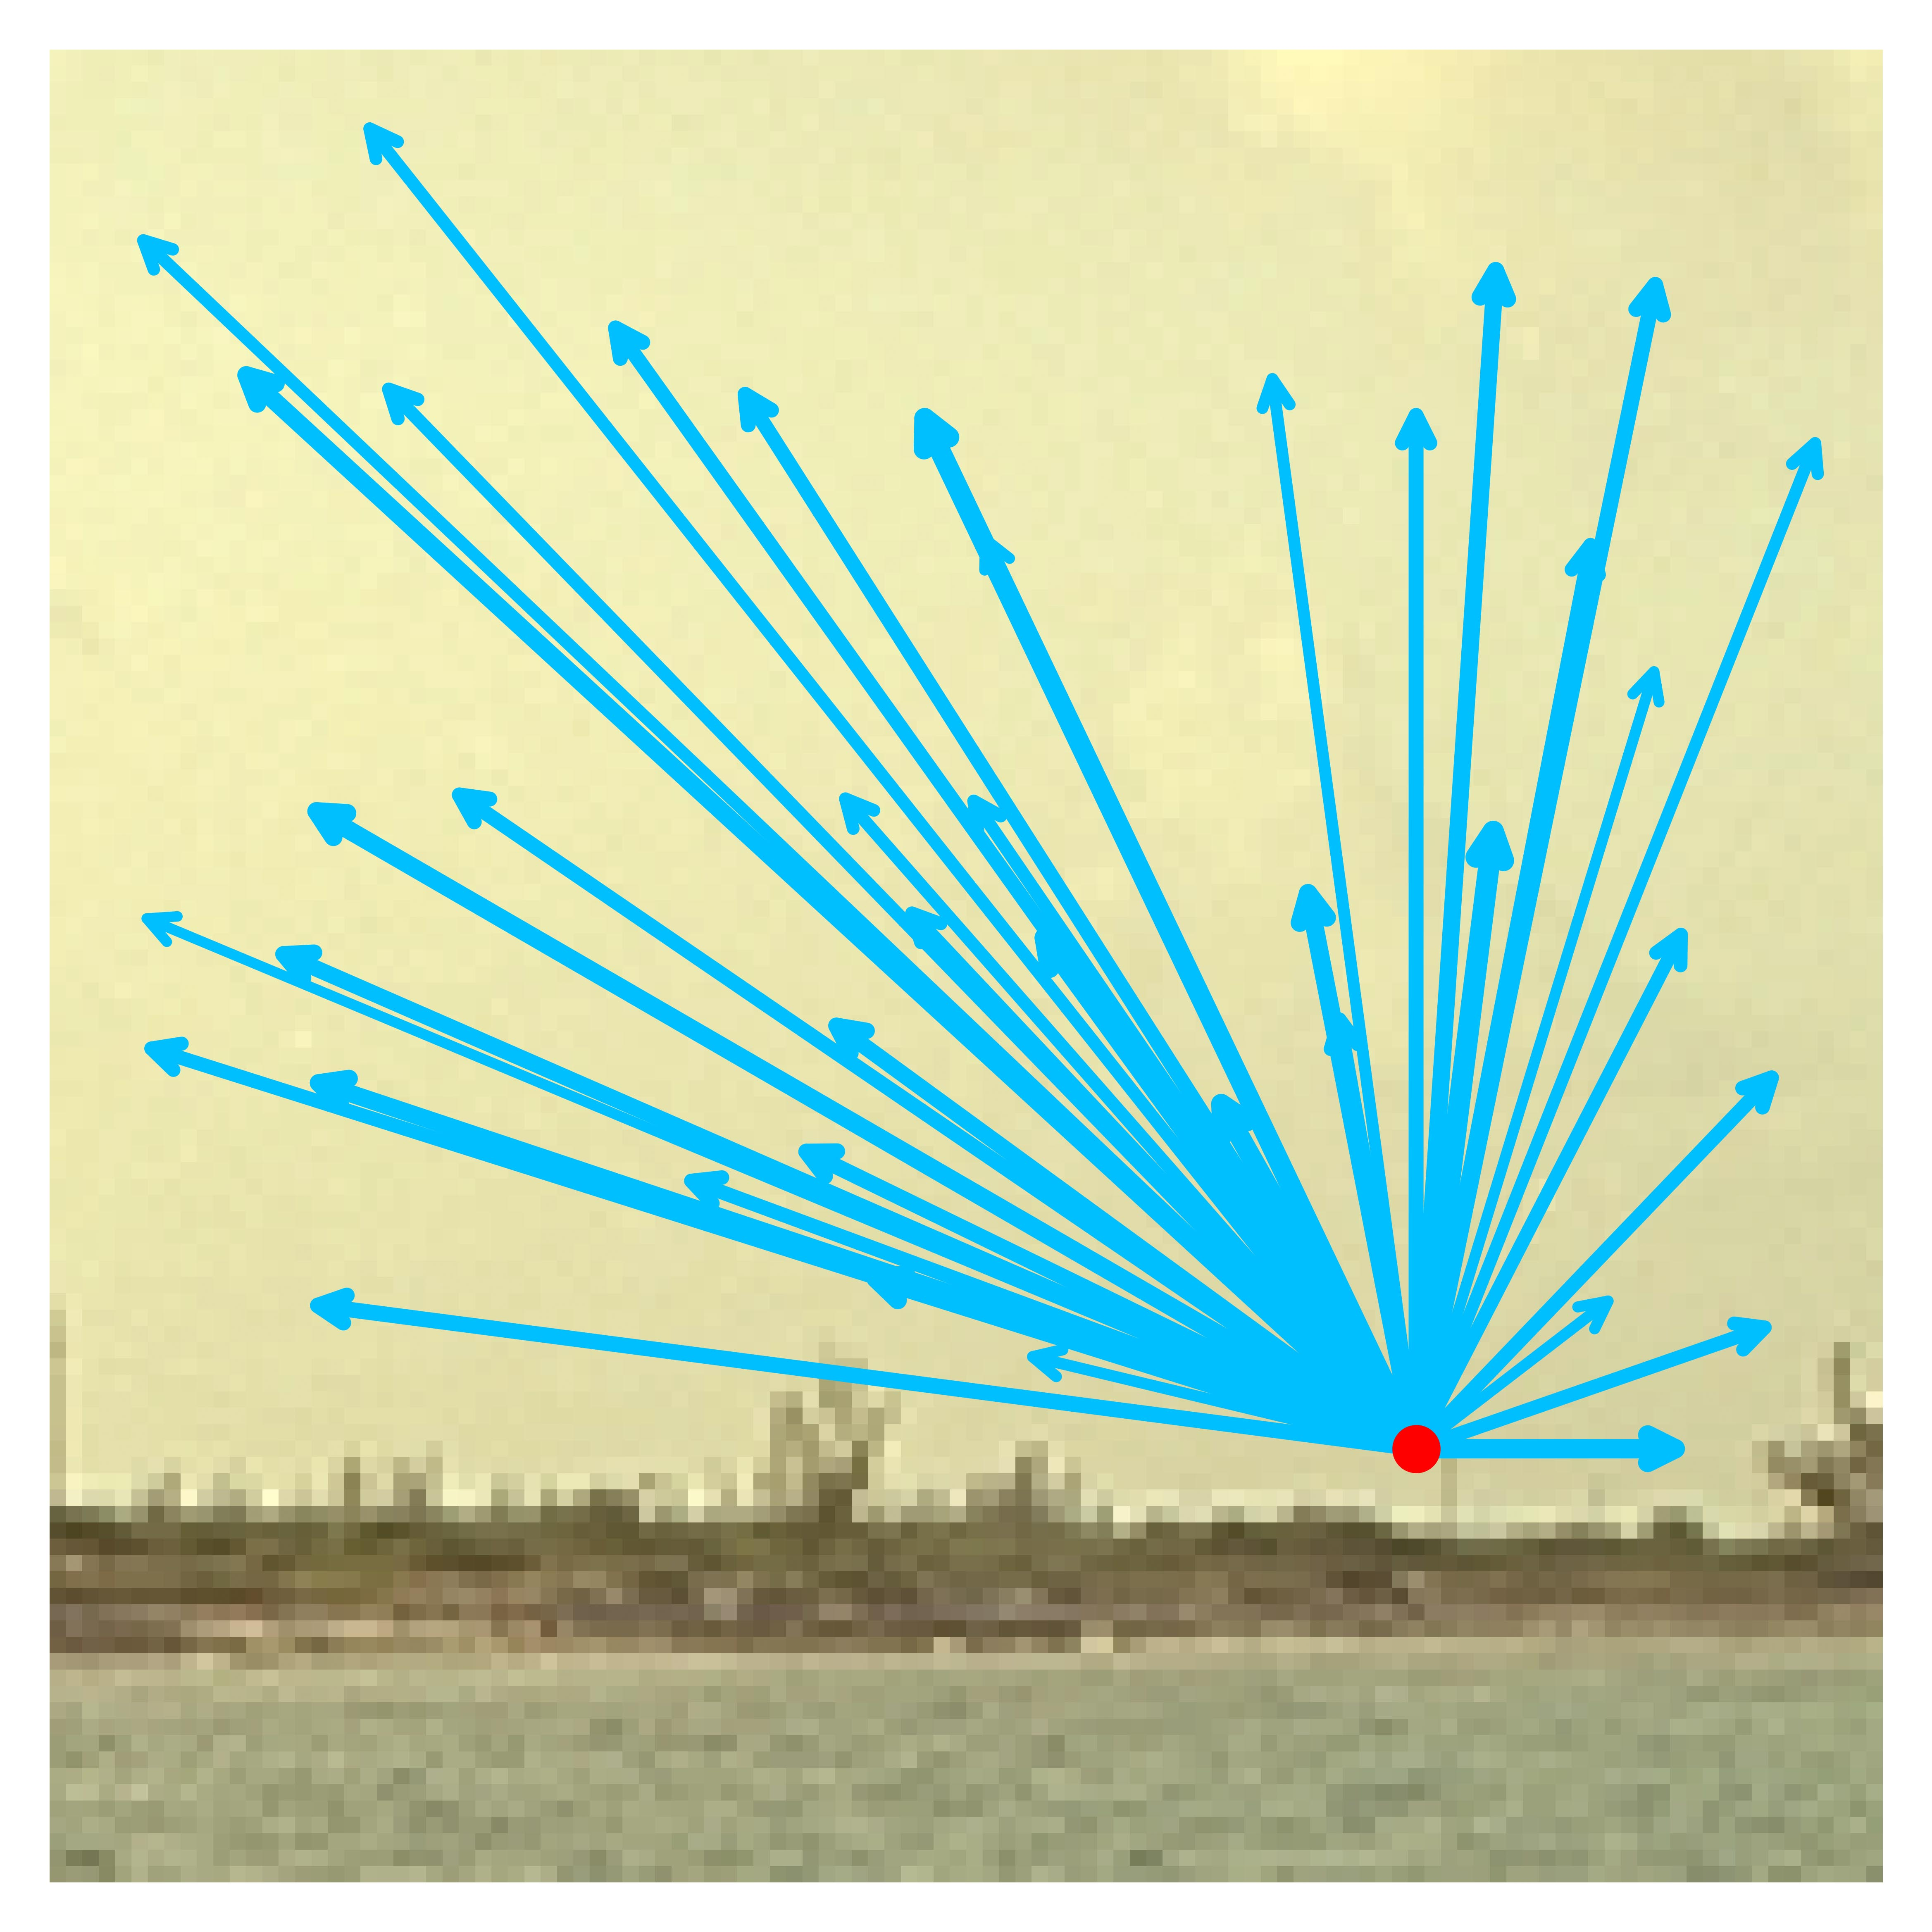
\includegraphics[width=1.5in]{cropped/boat_superpixel_3.jpg}
			\centerline{(g)}
			\label{BOAT-3}
		\end{minipage}
		\begin{minipage}[t]{.24\linewidth}
			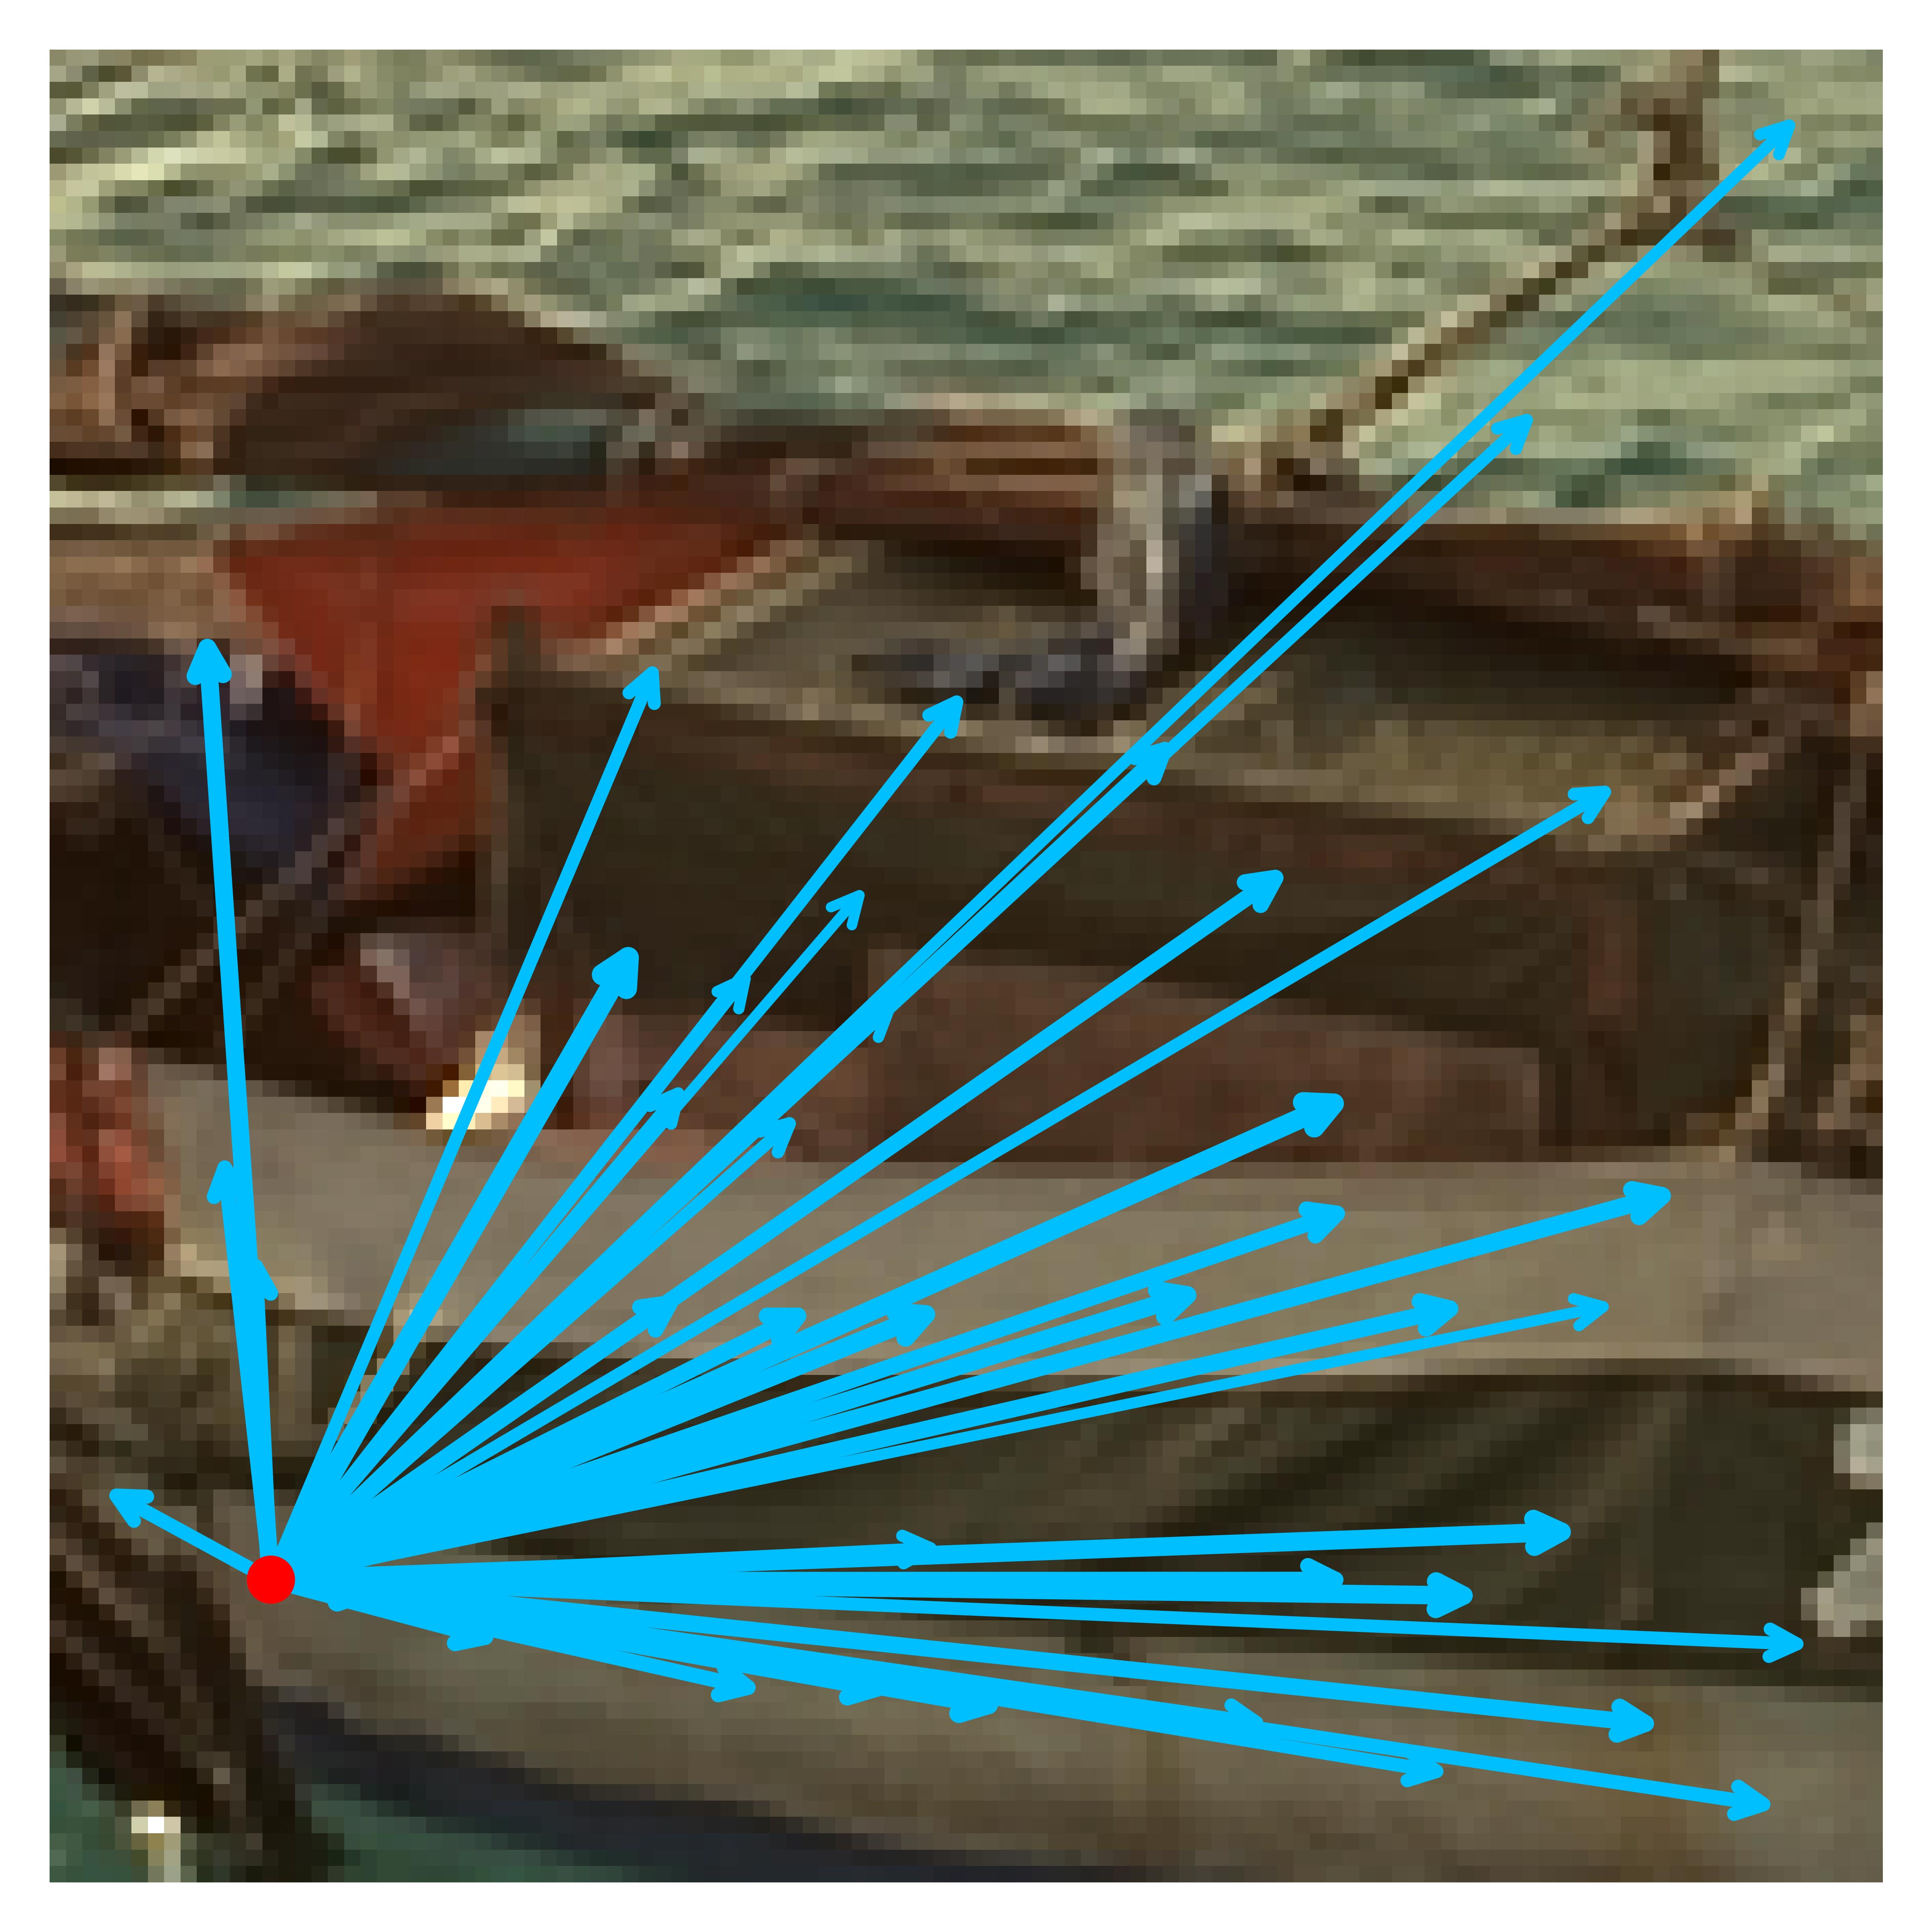
\includegraphics[width=1.5in]{cropped/boat_superpixel_9.jpg}
			\centerline{(h)}
			\label{BOAT-4}
		\end{minipage}
		\begin{minipage}[t]{.24\linewidth}
			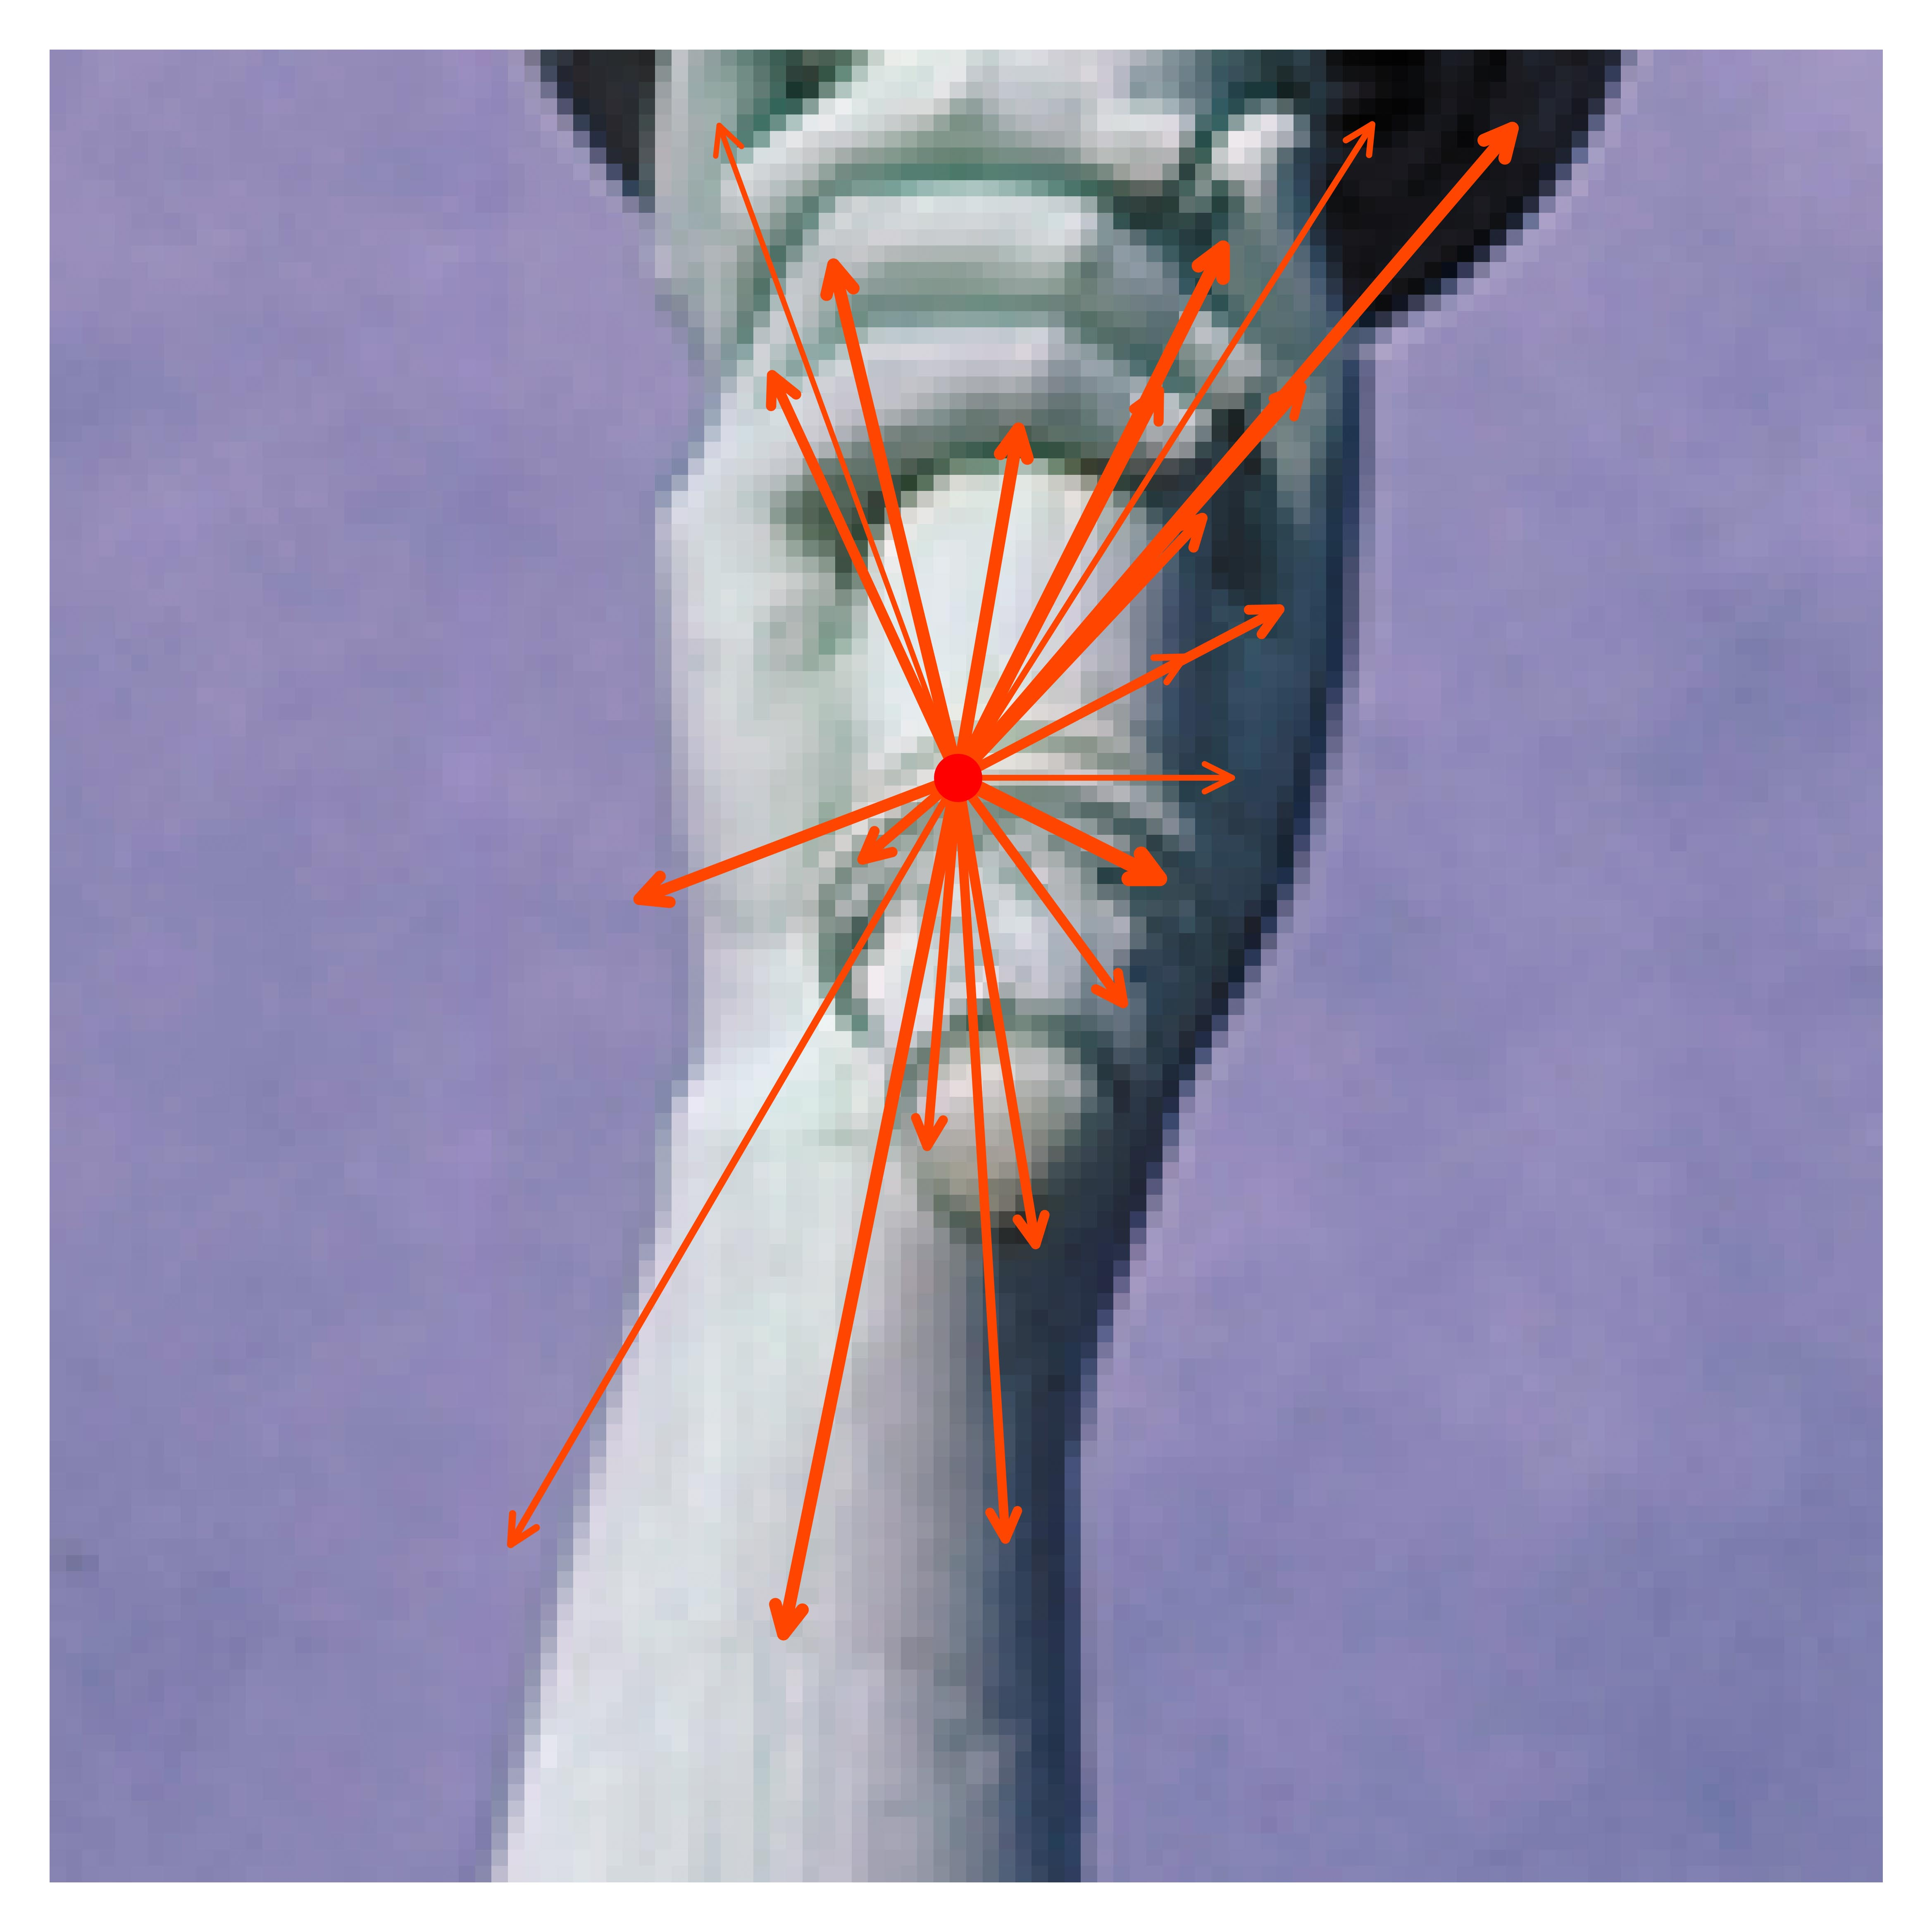
\includegraphics[width=1.5in]{cropped/lady_superpixel_1.jpg}
			\centerline{(i)}
			\label{LADY-1}
		\end{minipage}
		\begin{minipage}[t]{.24\linewidth}
			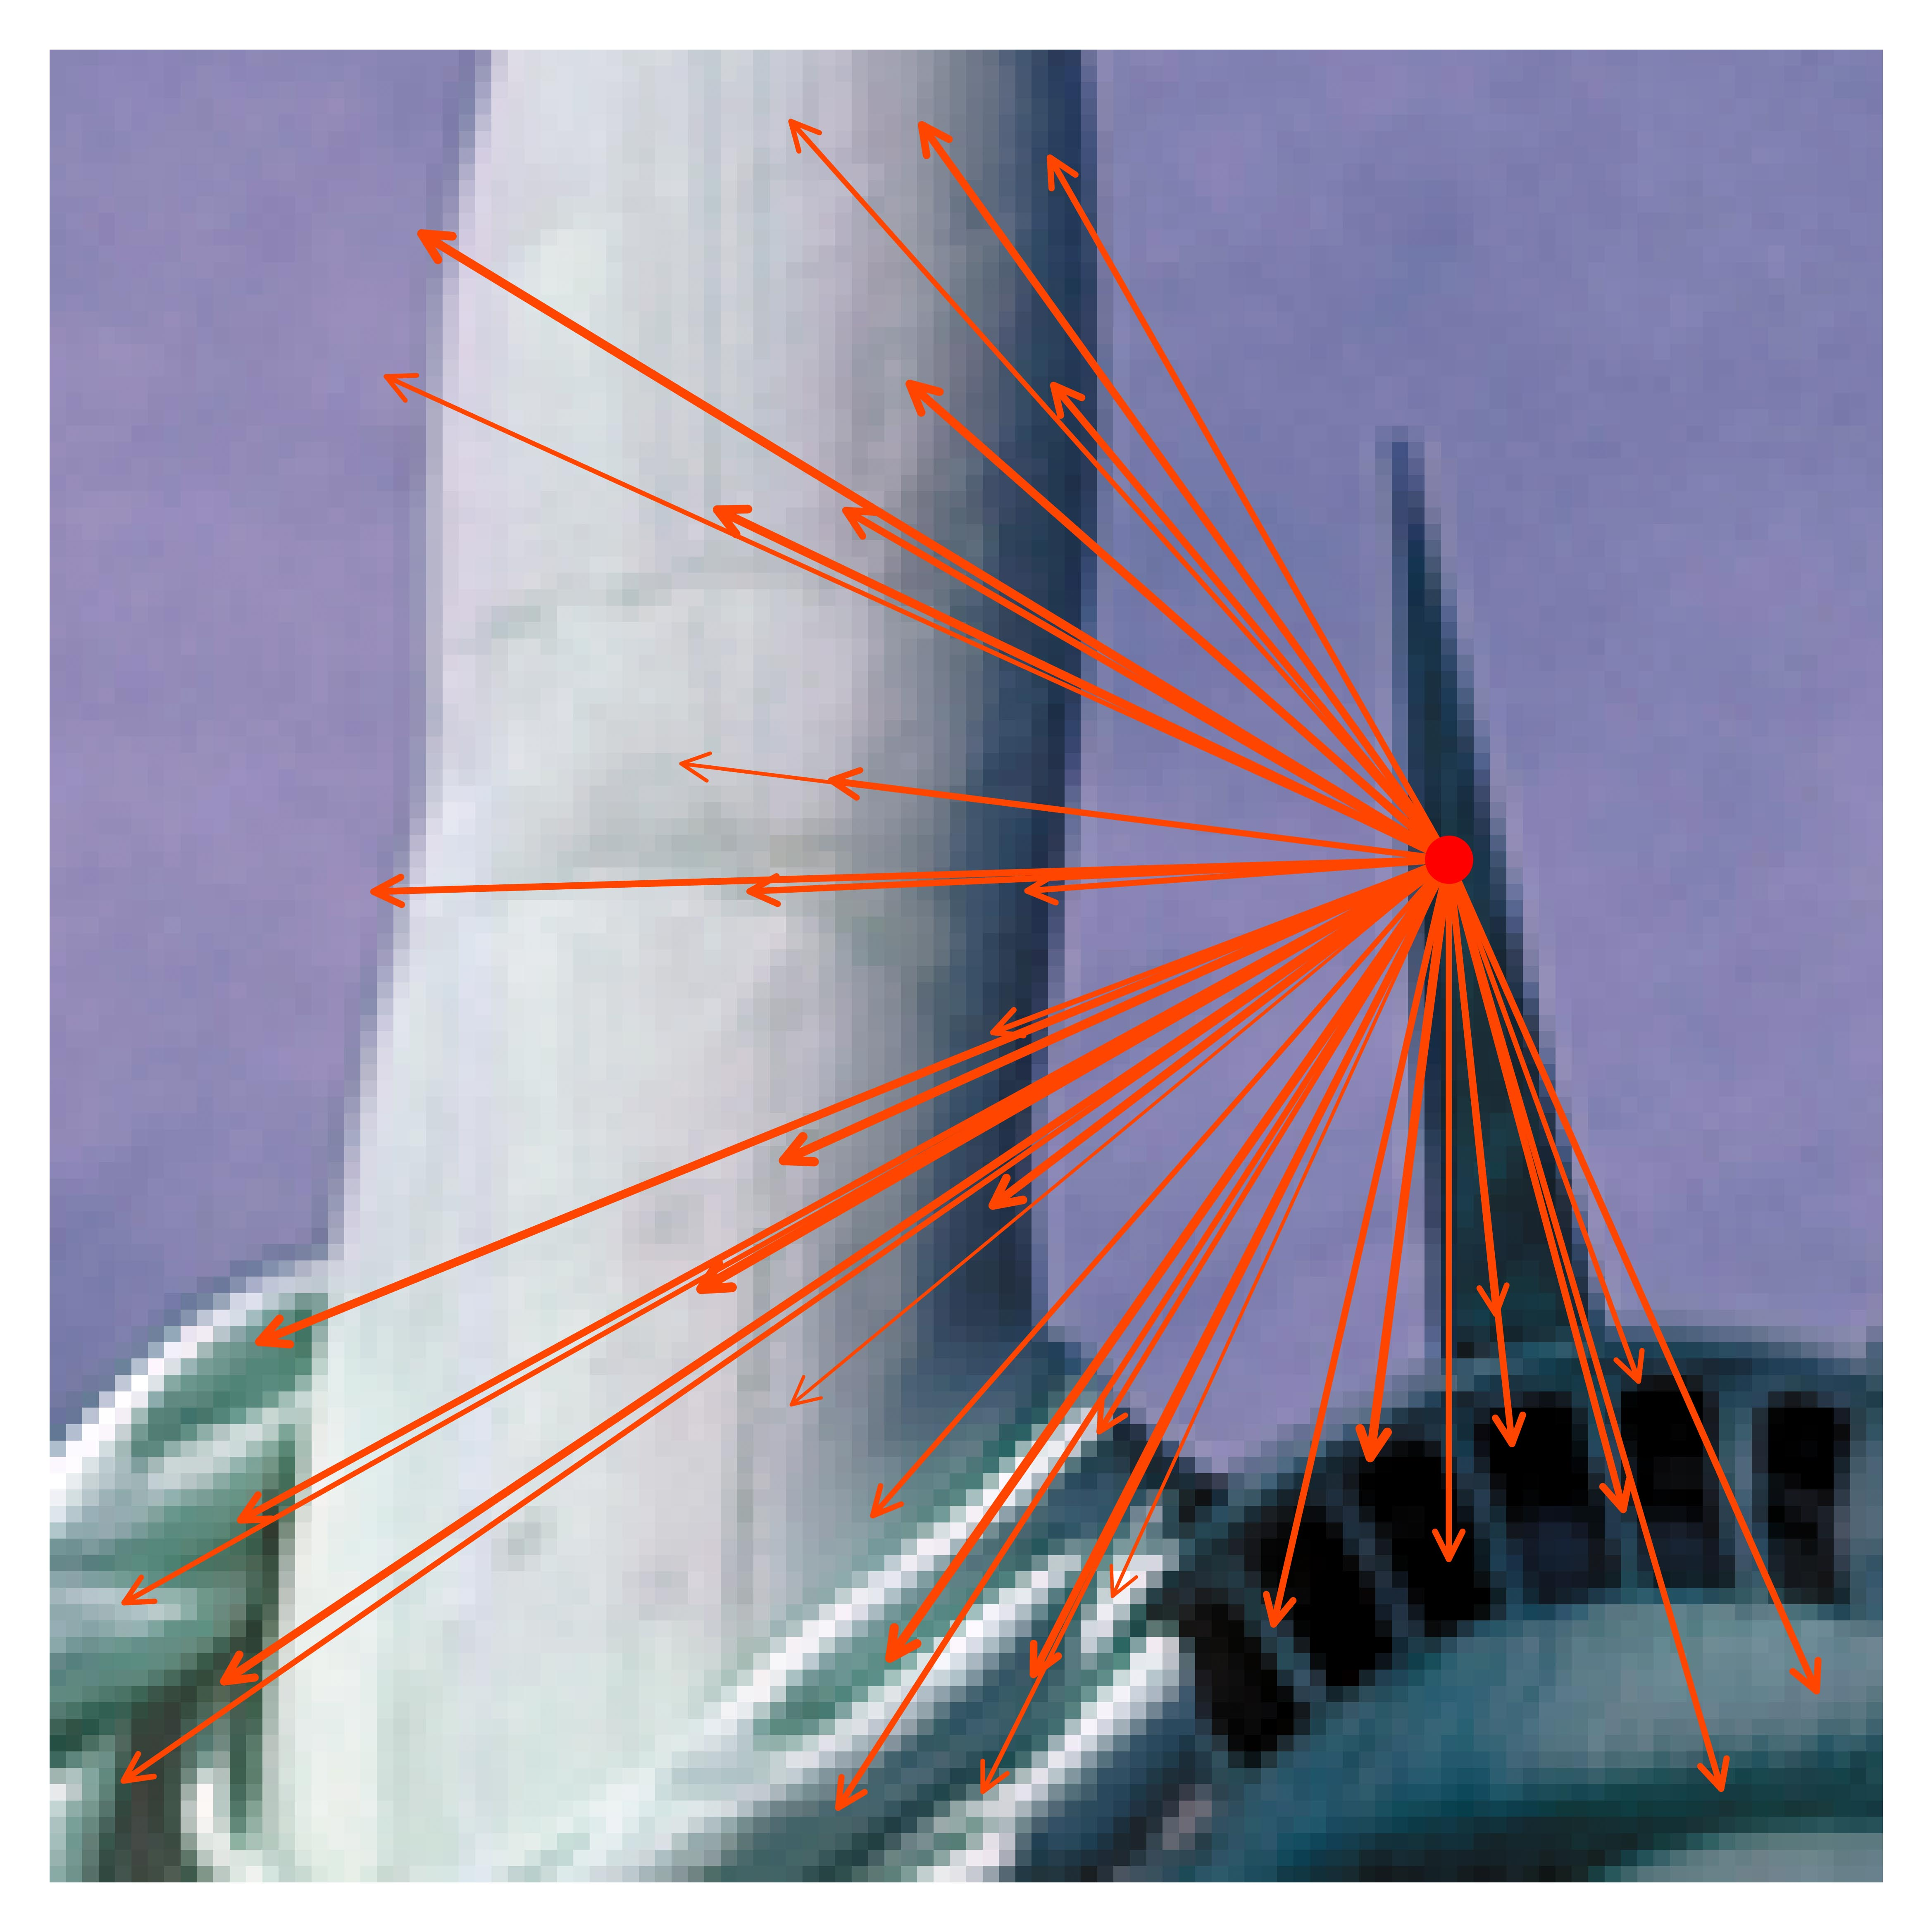
\includegraphics[width=1.5in]{cropped/lady_superpixel_5.jpg}
			\centerline{(j)}
			\label{LADY-2}
		\end{minipage}
		\begin{minipage}[t]{.24\linewidth}
			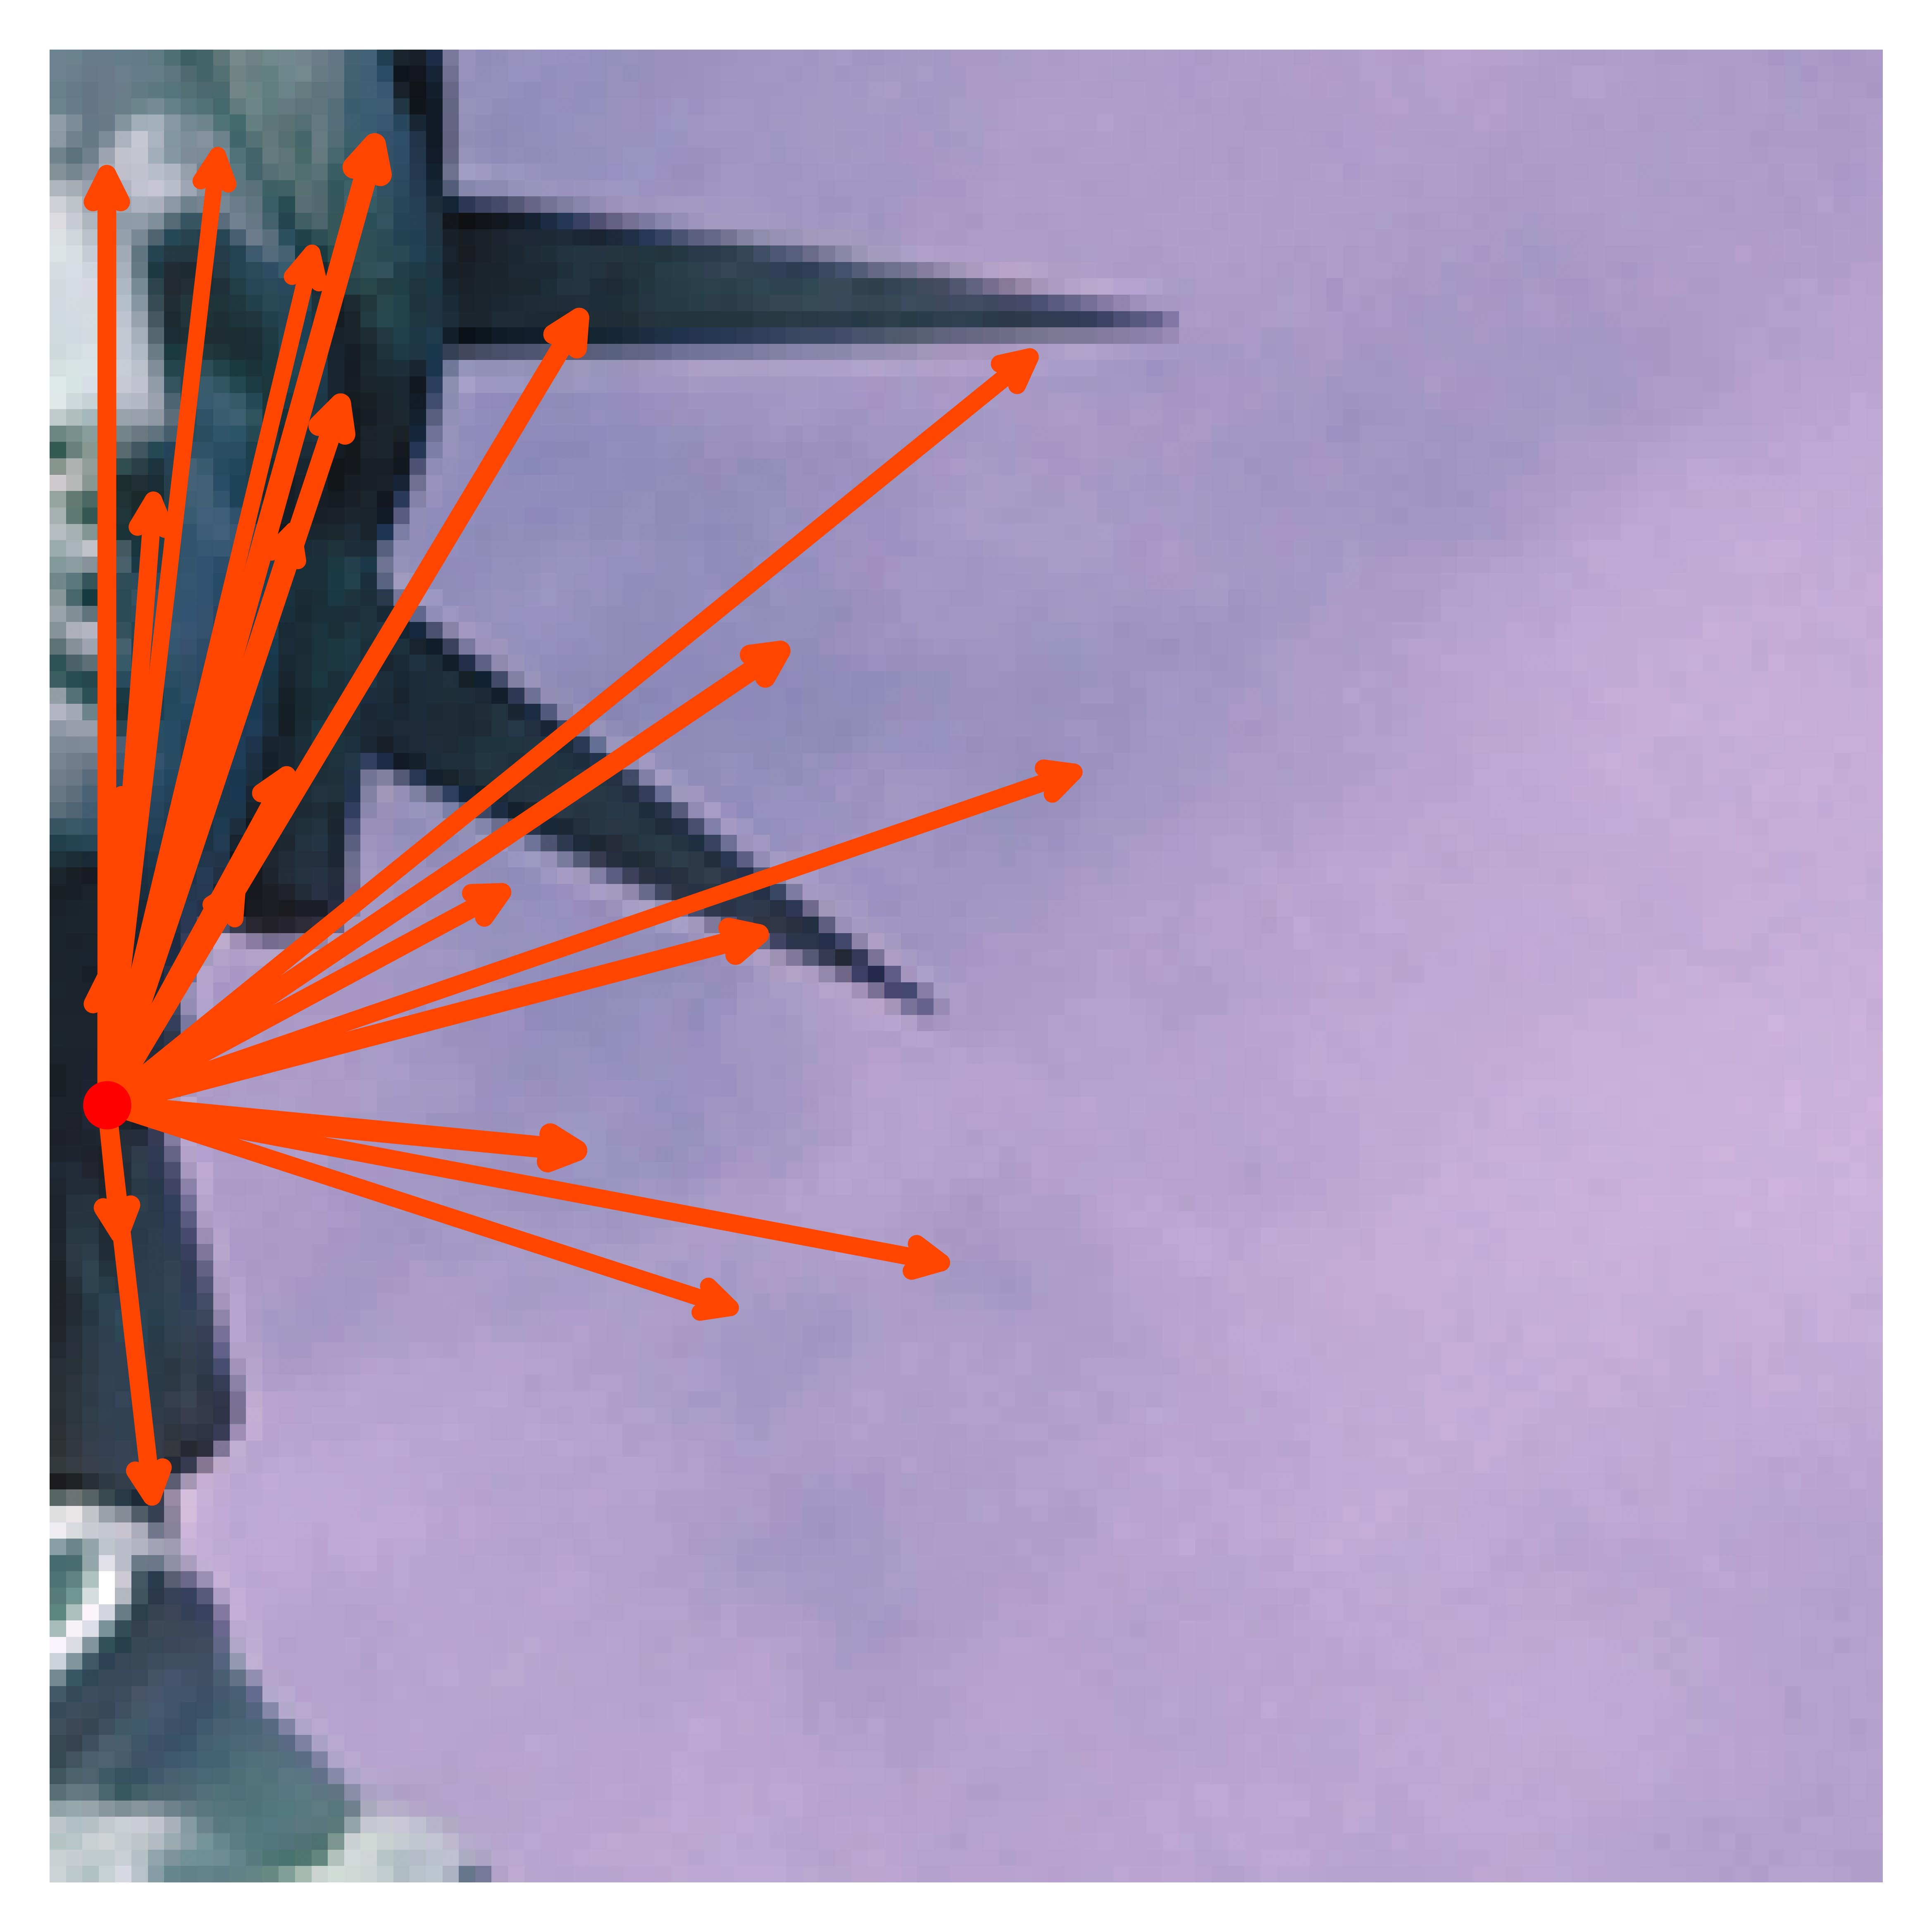
\includegraphics[width=1.5in]{cropped/lady_superpixel_10.jpg}
			\centerline{(k)}
			\label{LADY-3}
		\end{minipage}
		\begin{minipage}[t]{.24\linewidth}
			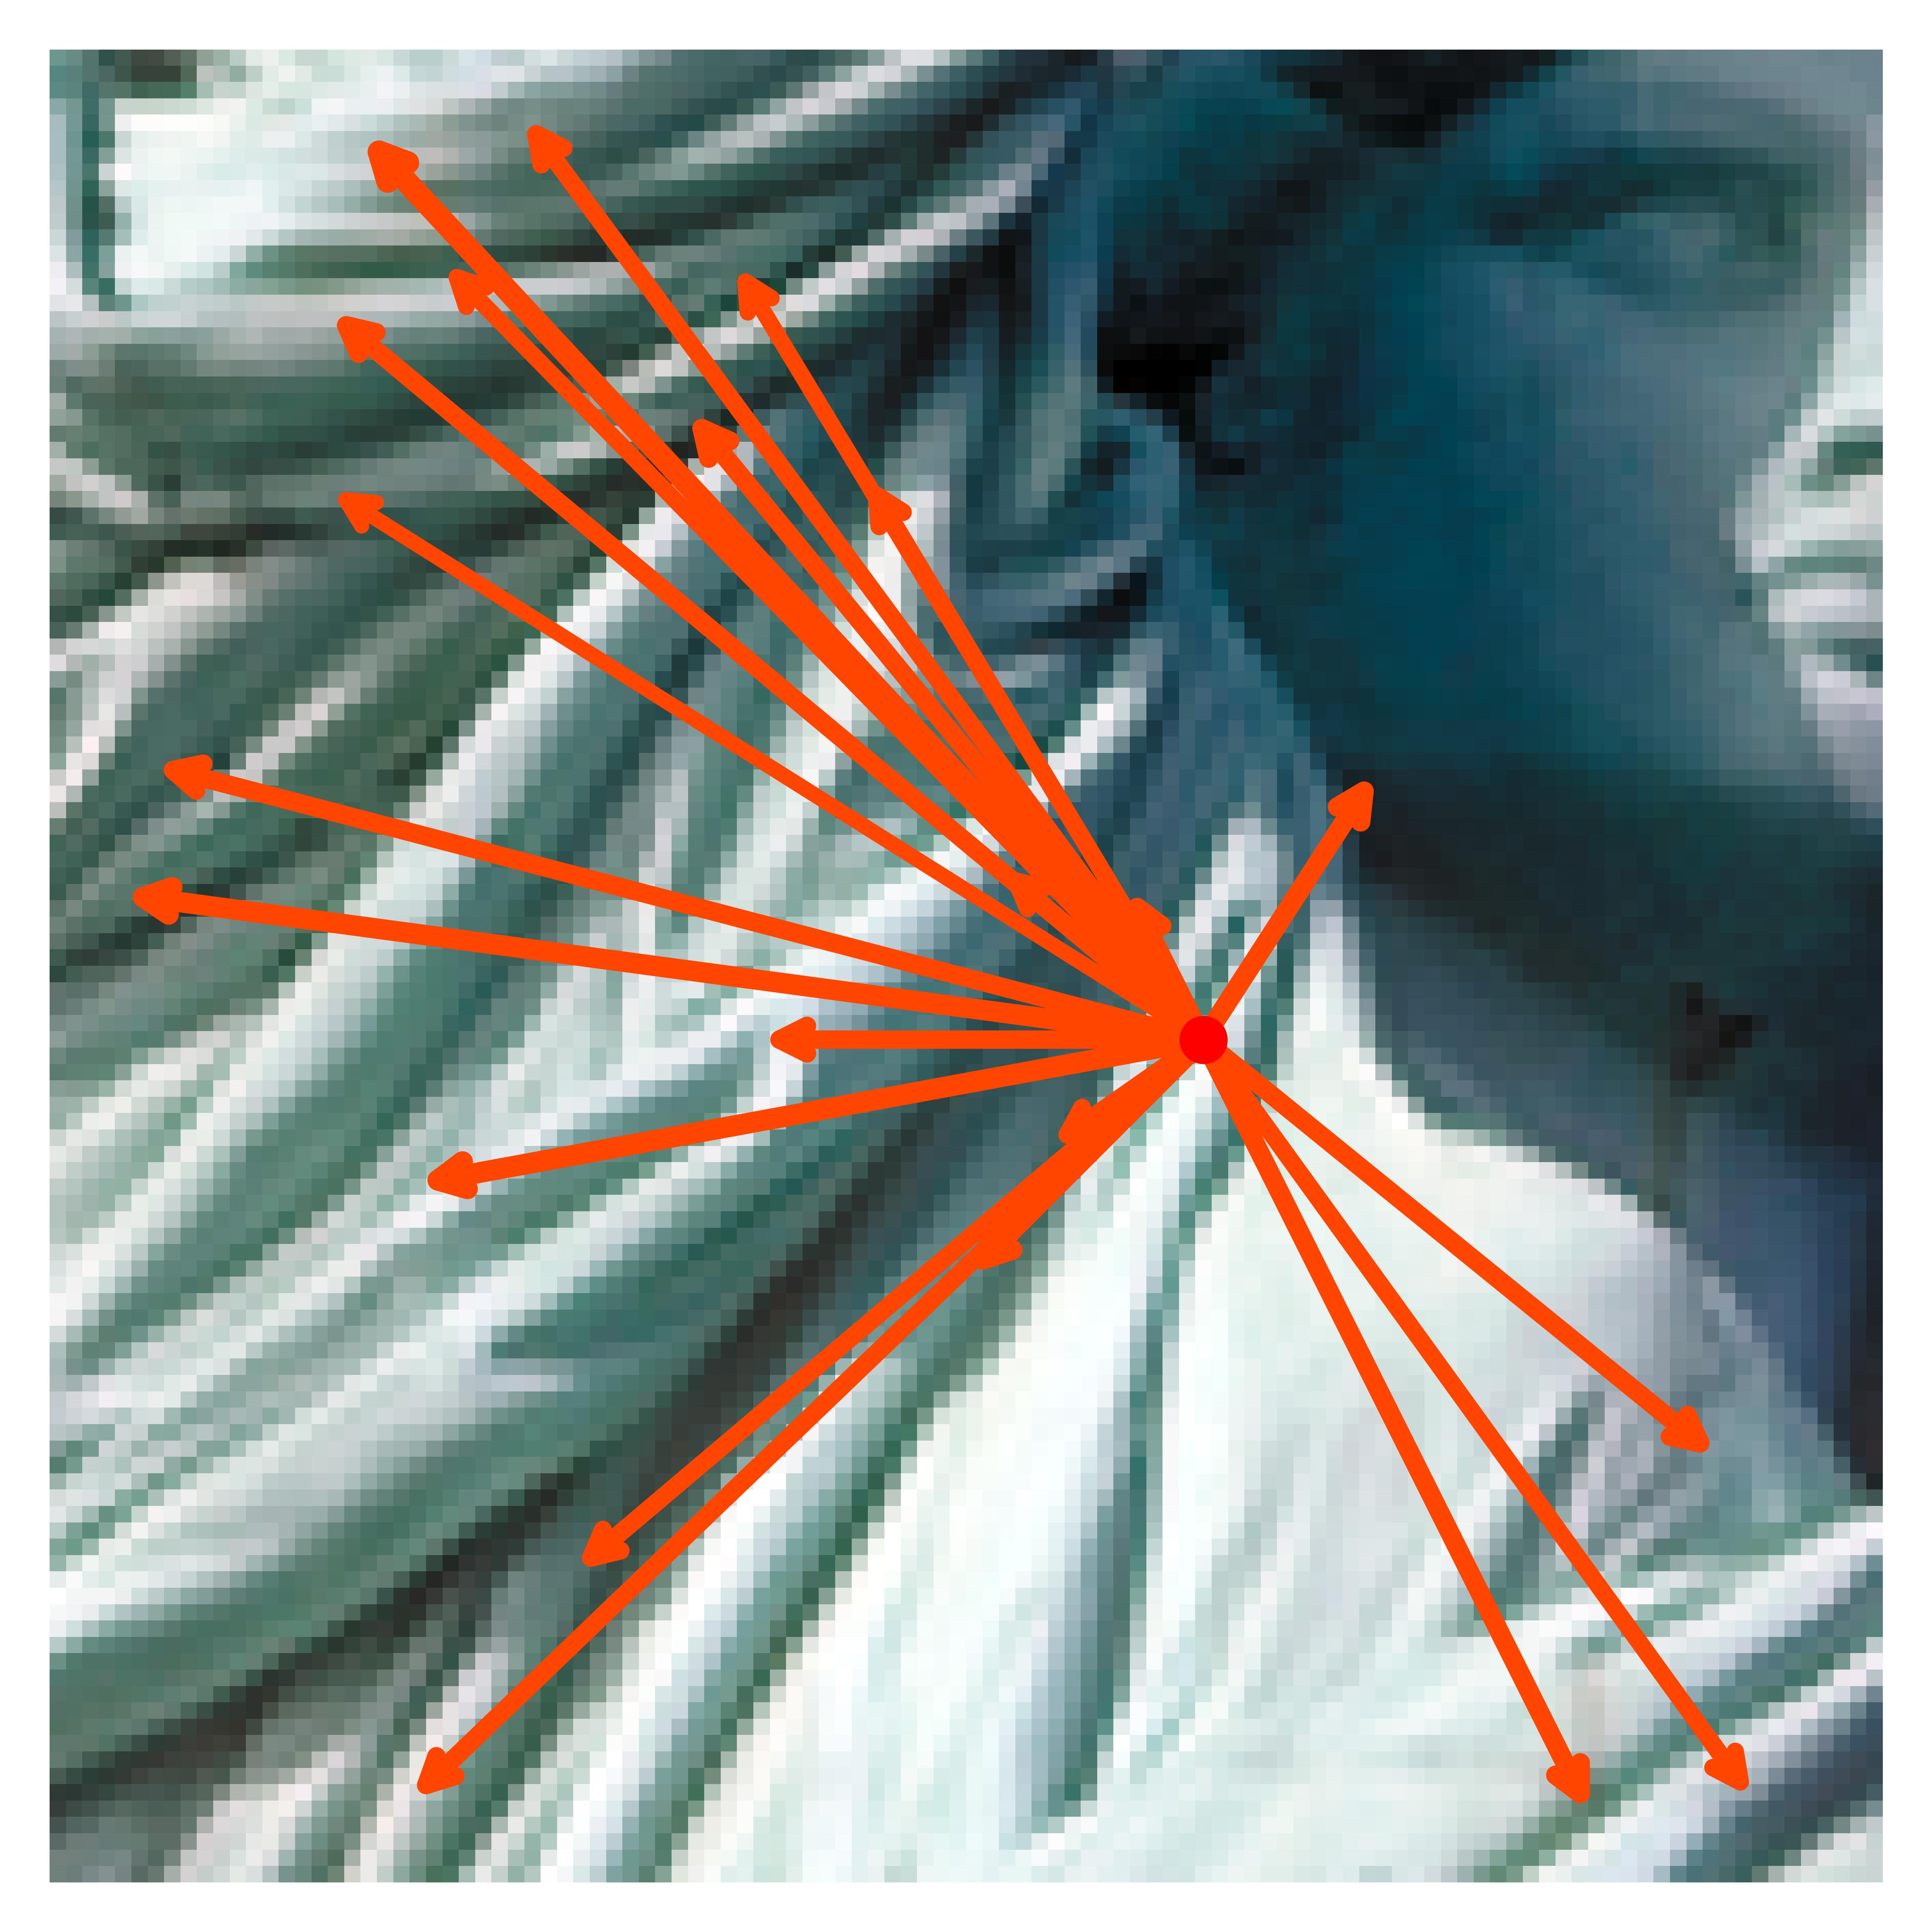
\includegraphics[width=1.5in]{cropped/lady_superpixel_9.jpg}
			\centerline{(l)}
			\label{LADY-4}
		\end{minipage}
		\begin{minipage}[t]{.24\linewidth}
			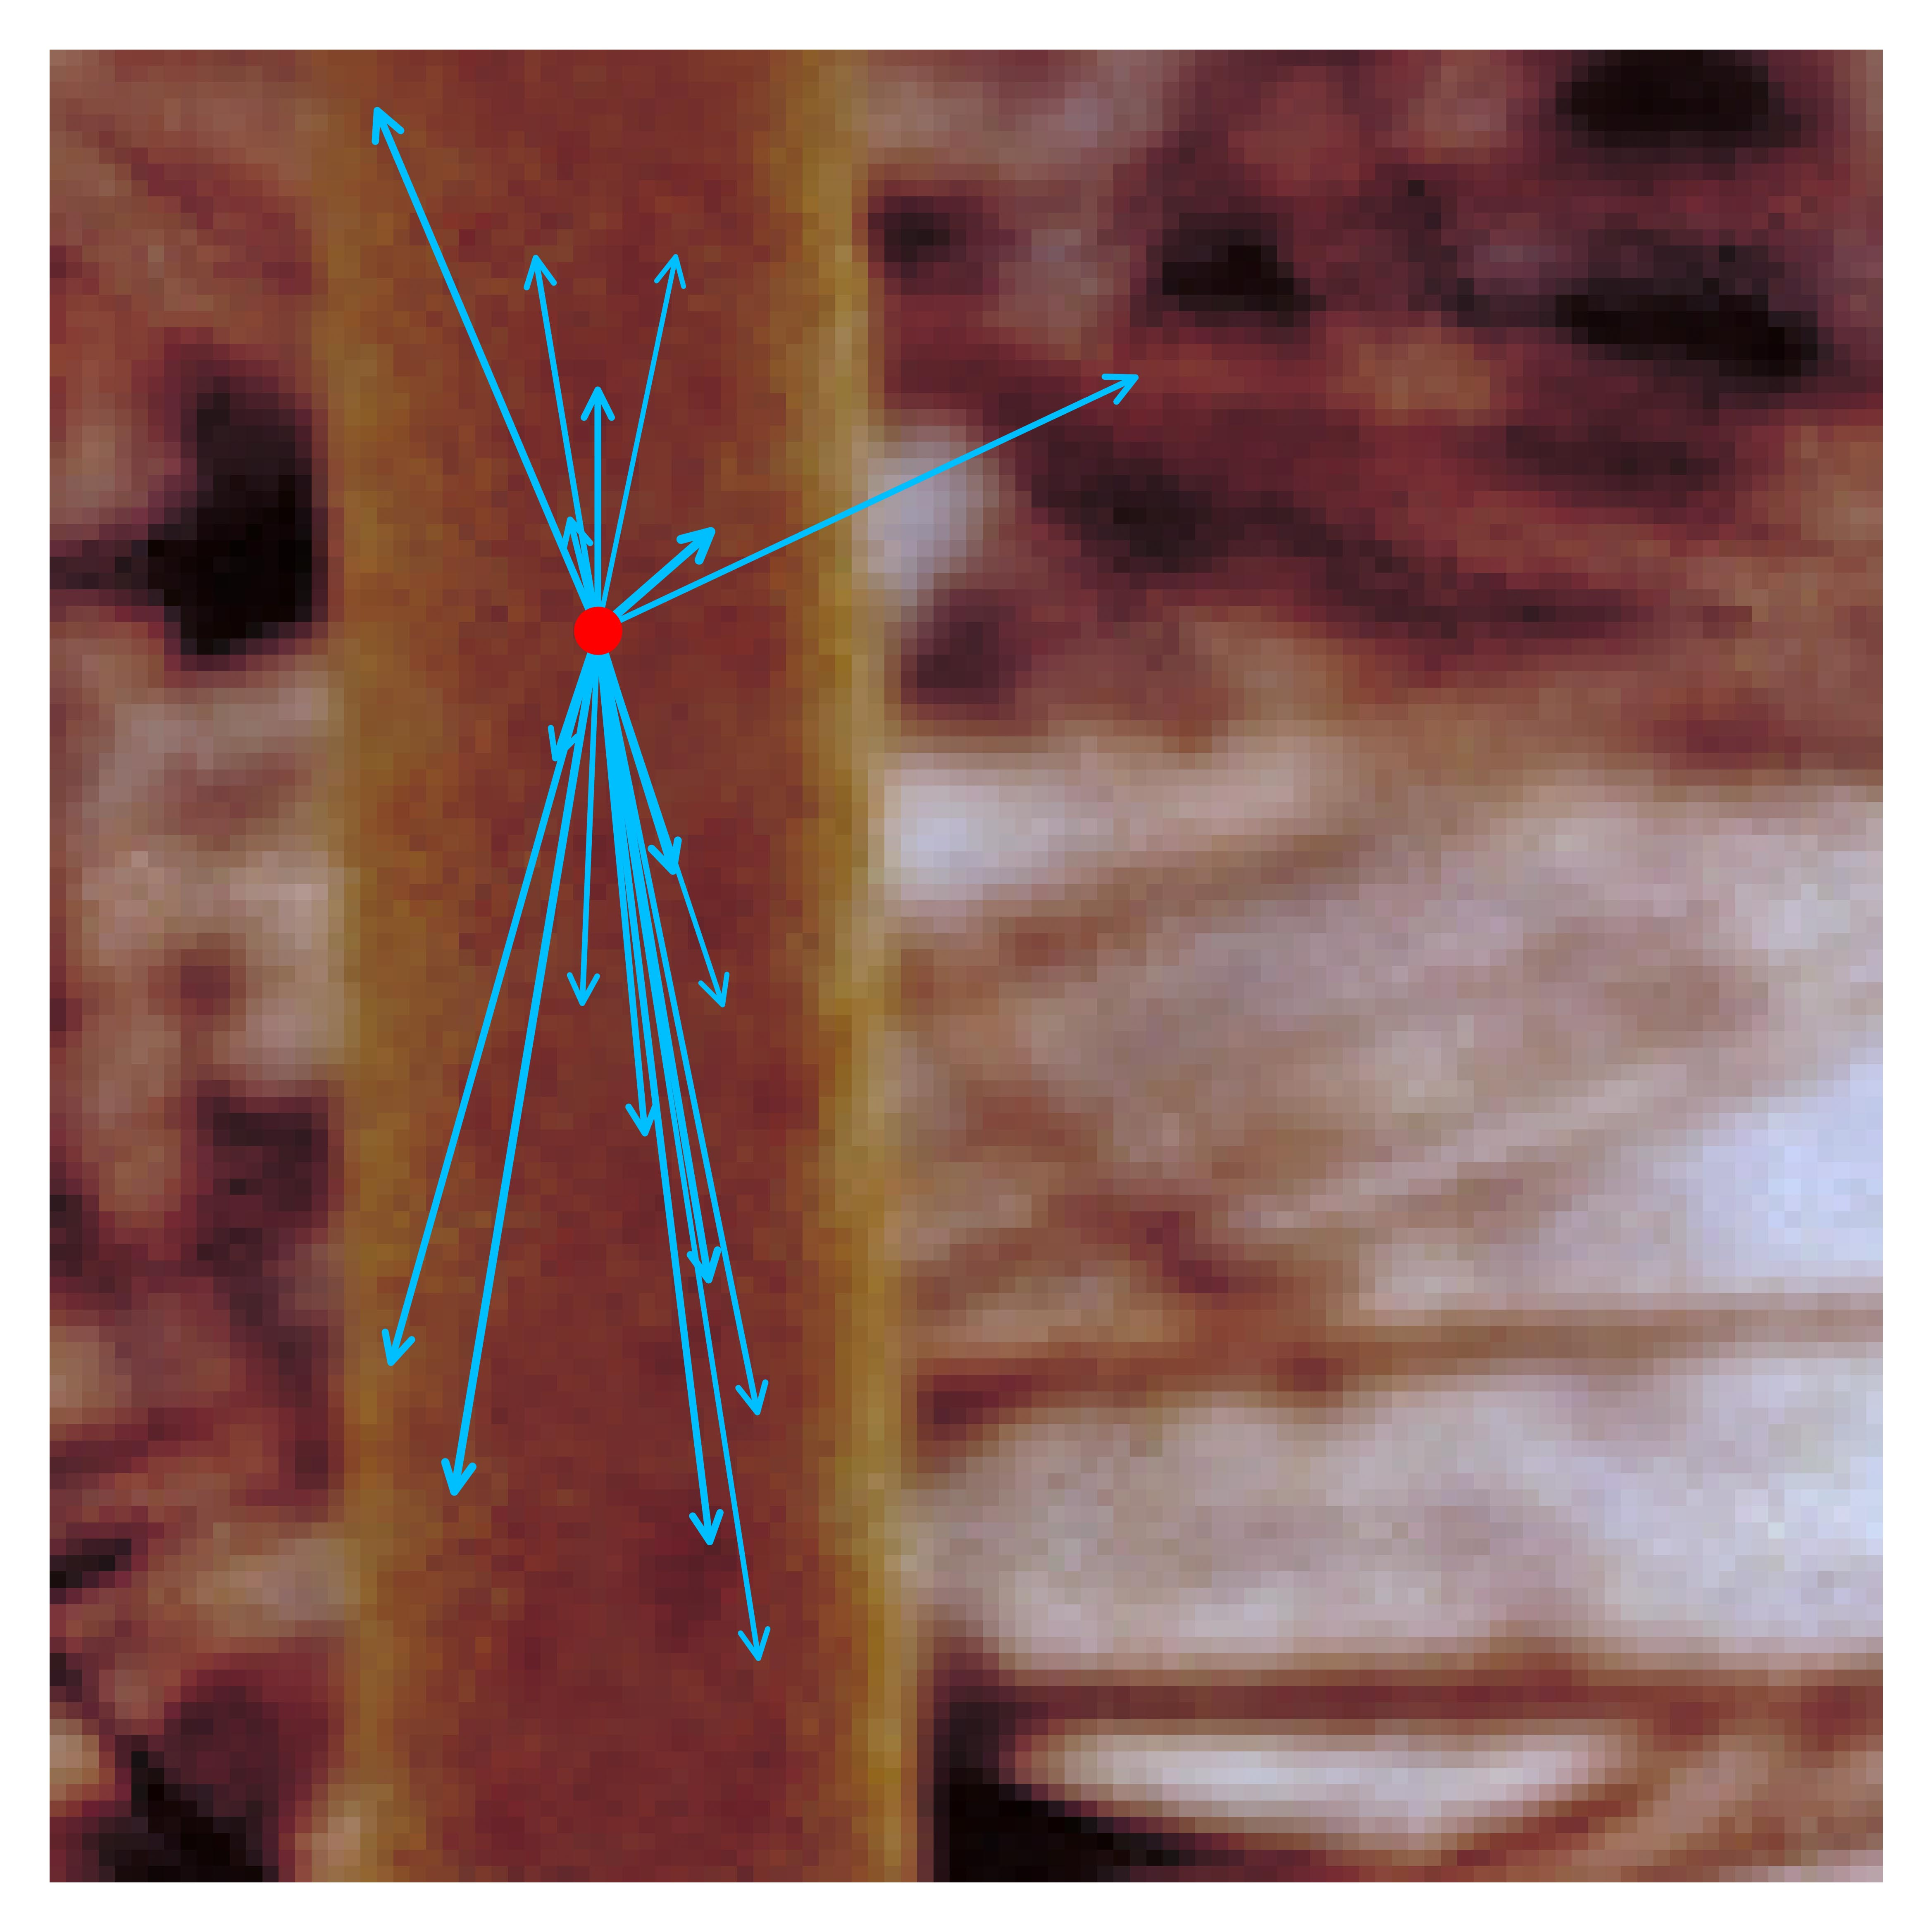
\includegraphics[width=1.5in]{cropped/shroom_superpixel_9.jpg}
			\centerline{(m)}
			\label{SHROOM-1}
		\end{minipage}
		\begin{minipage}[t]{.24\linewidth}
			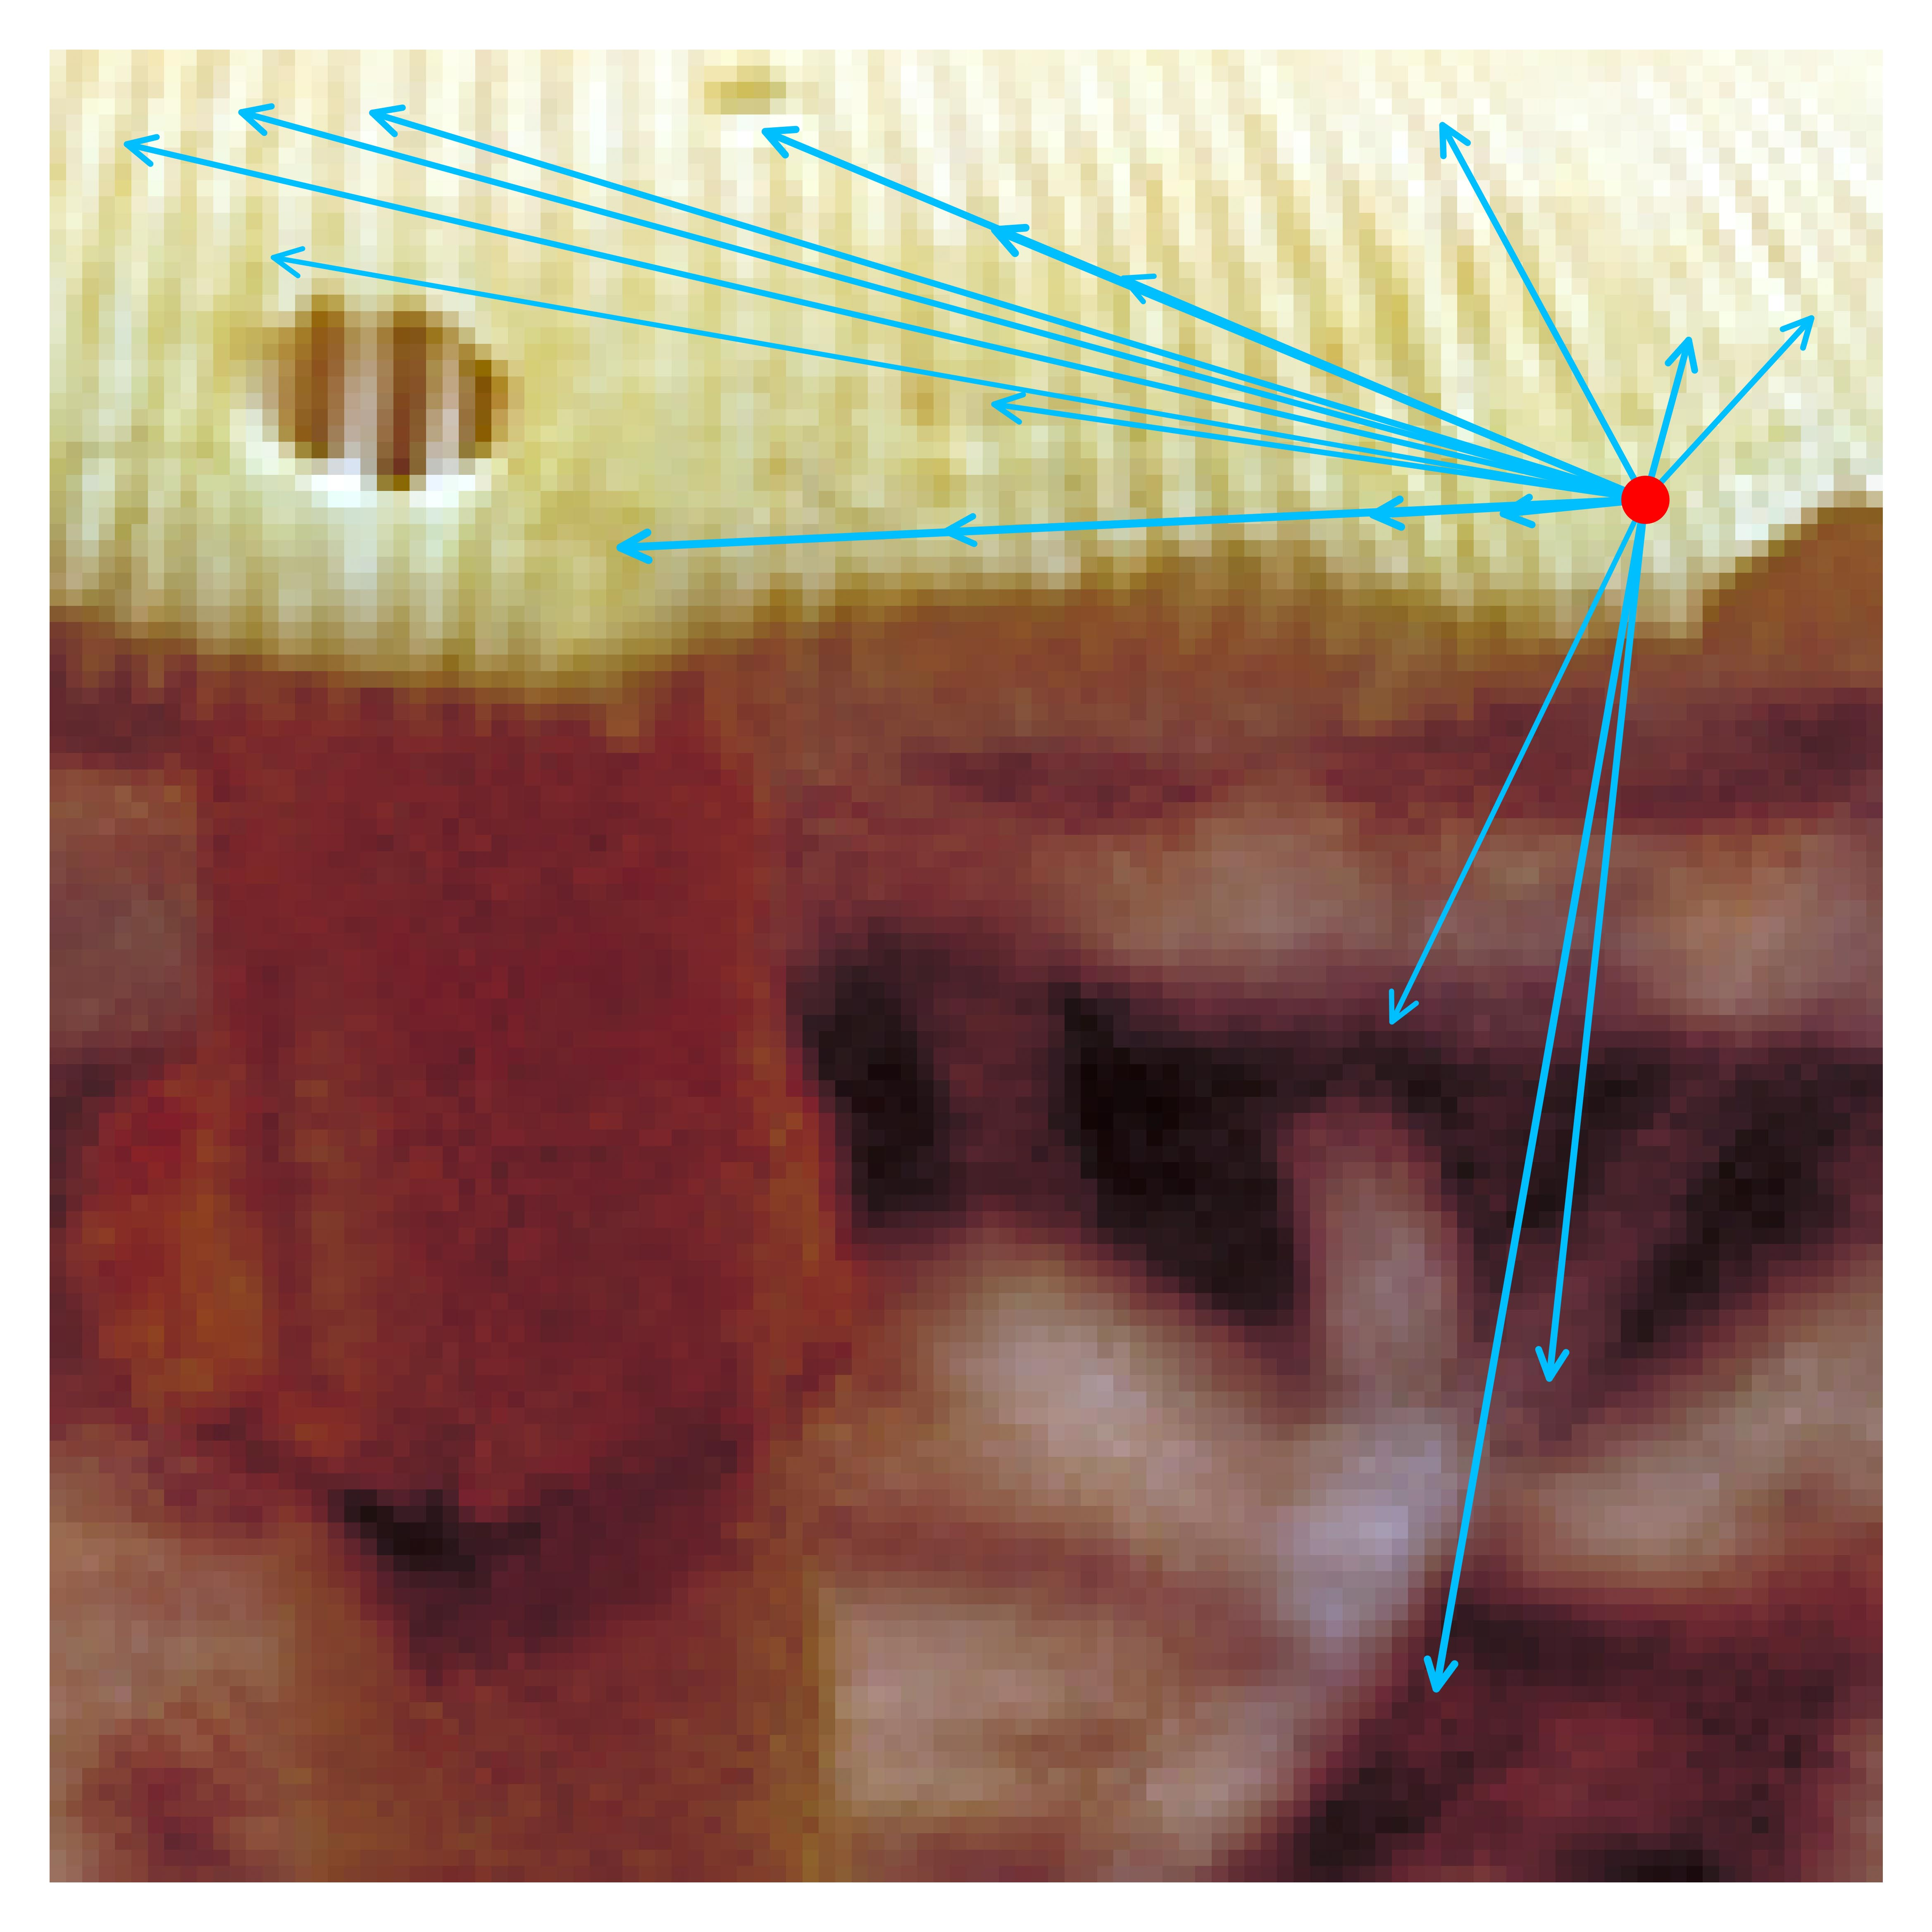
\includegraphics[width=1.5in]{cropped/shroom_superpixel_5.jpg}
			\centerline{(n)}
			\label{SHROOM-2}
		\end{minipage}
		\begin{minipage}[t]{.24\linewidth}
			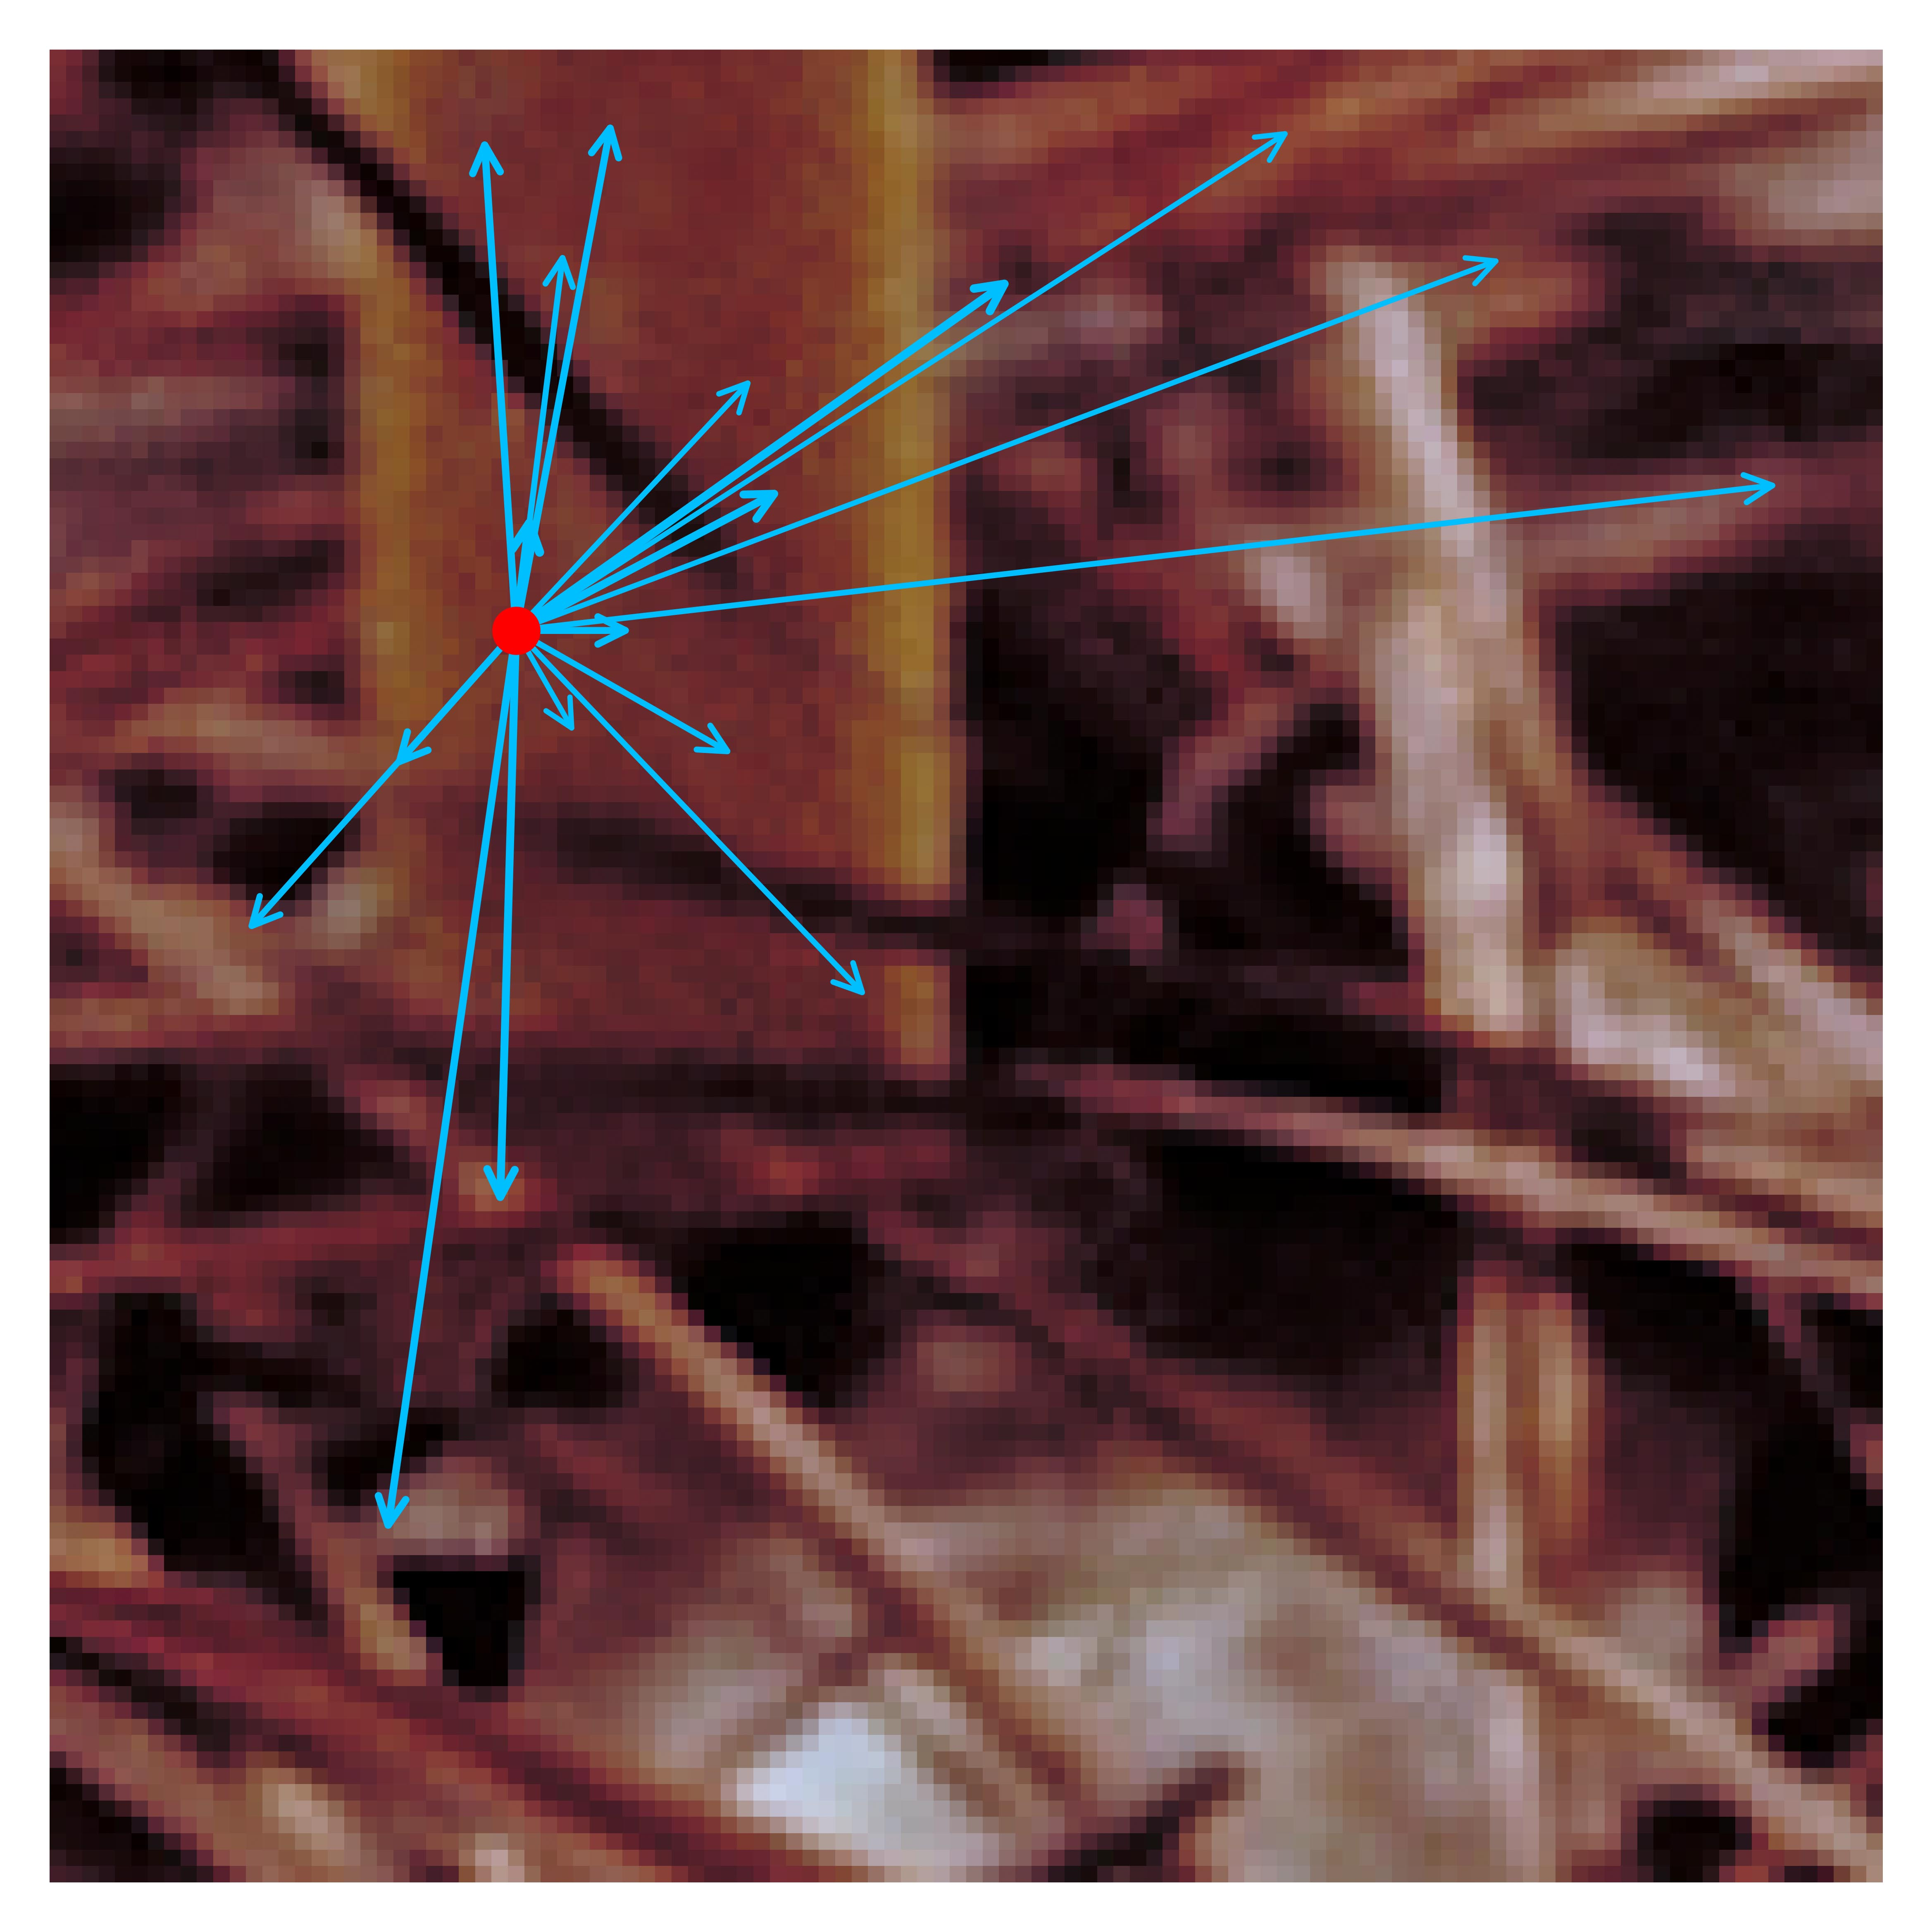
\includegraphics[width=1.5in]{cropped/shroom_superpixel_13.jpg}
			\centerline{(o)}
			\label{SHROOM-3}
		\end{minipage}
		\begin{minipage}[t]{.24\linewidth}
			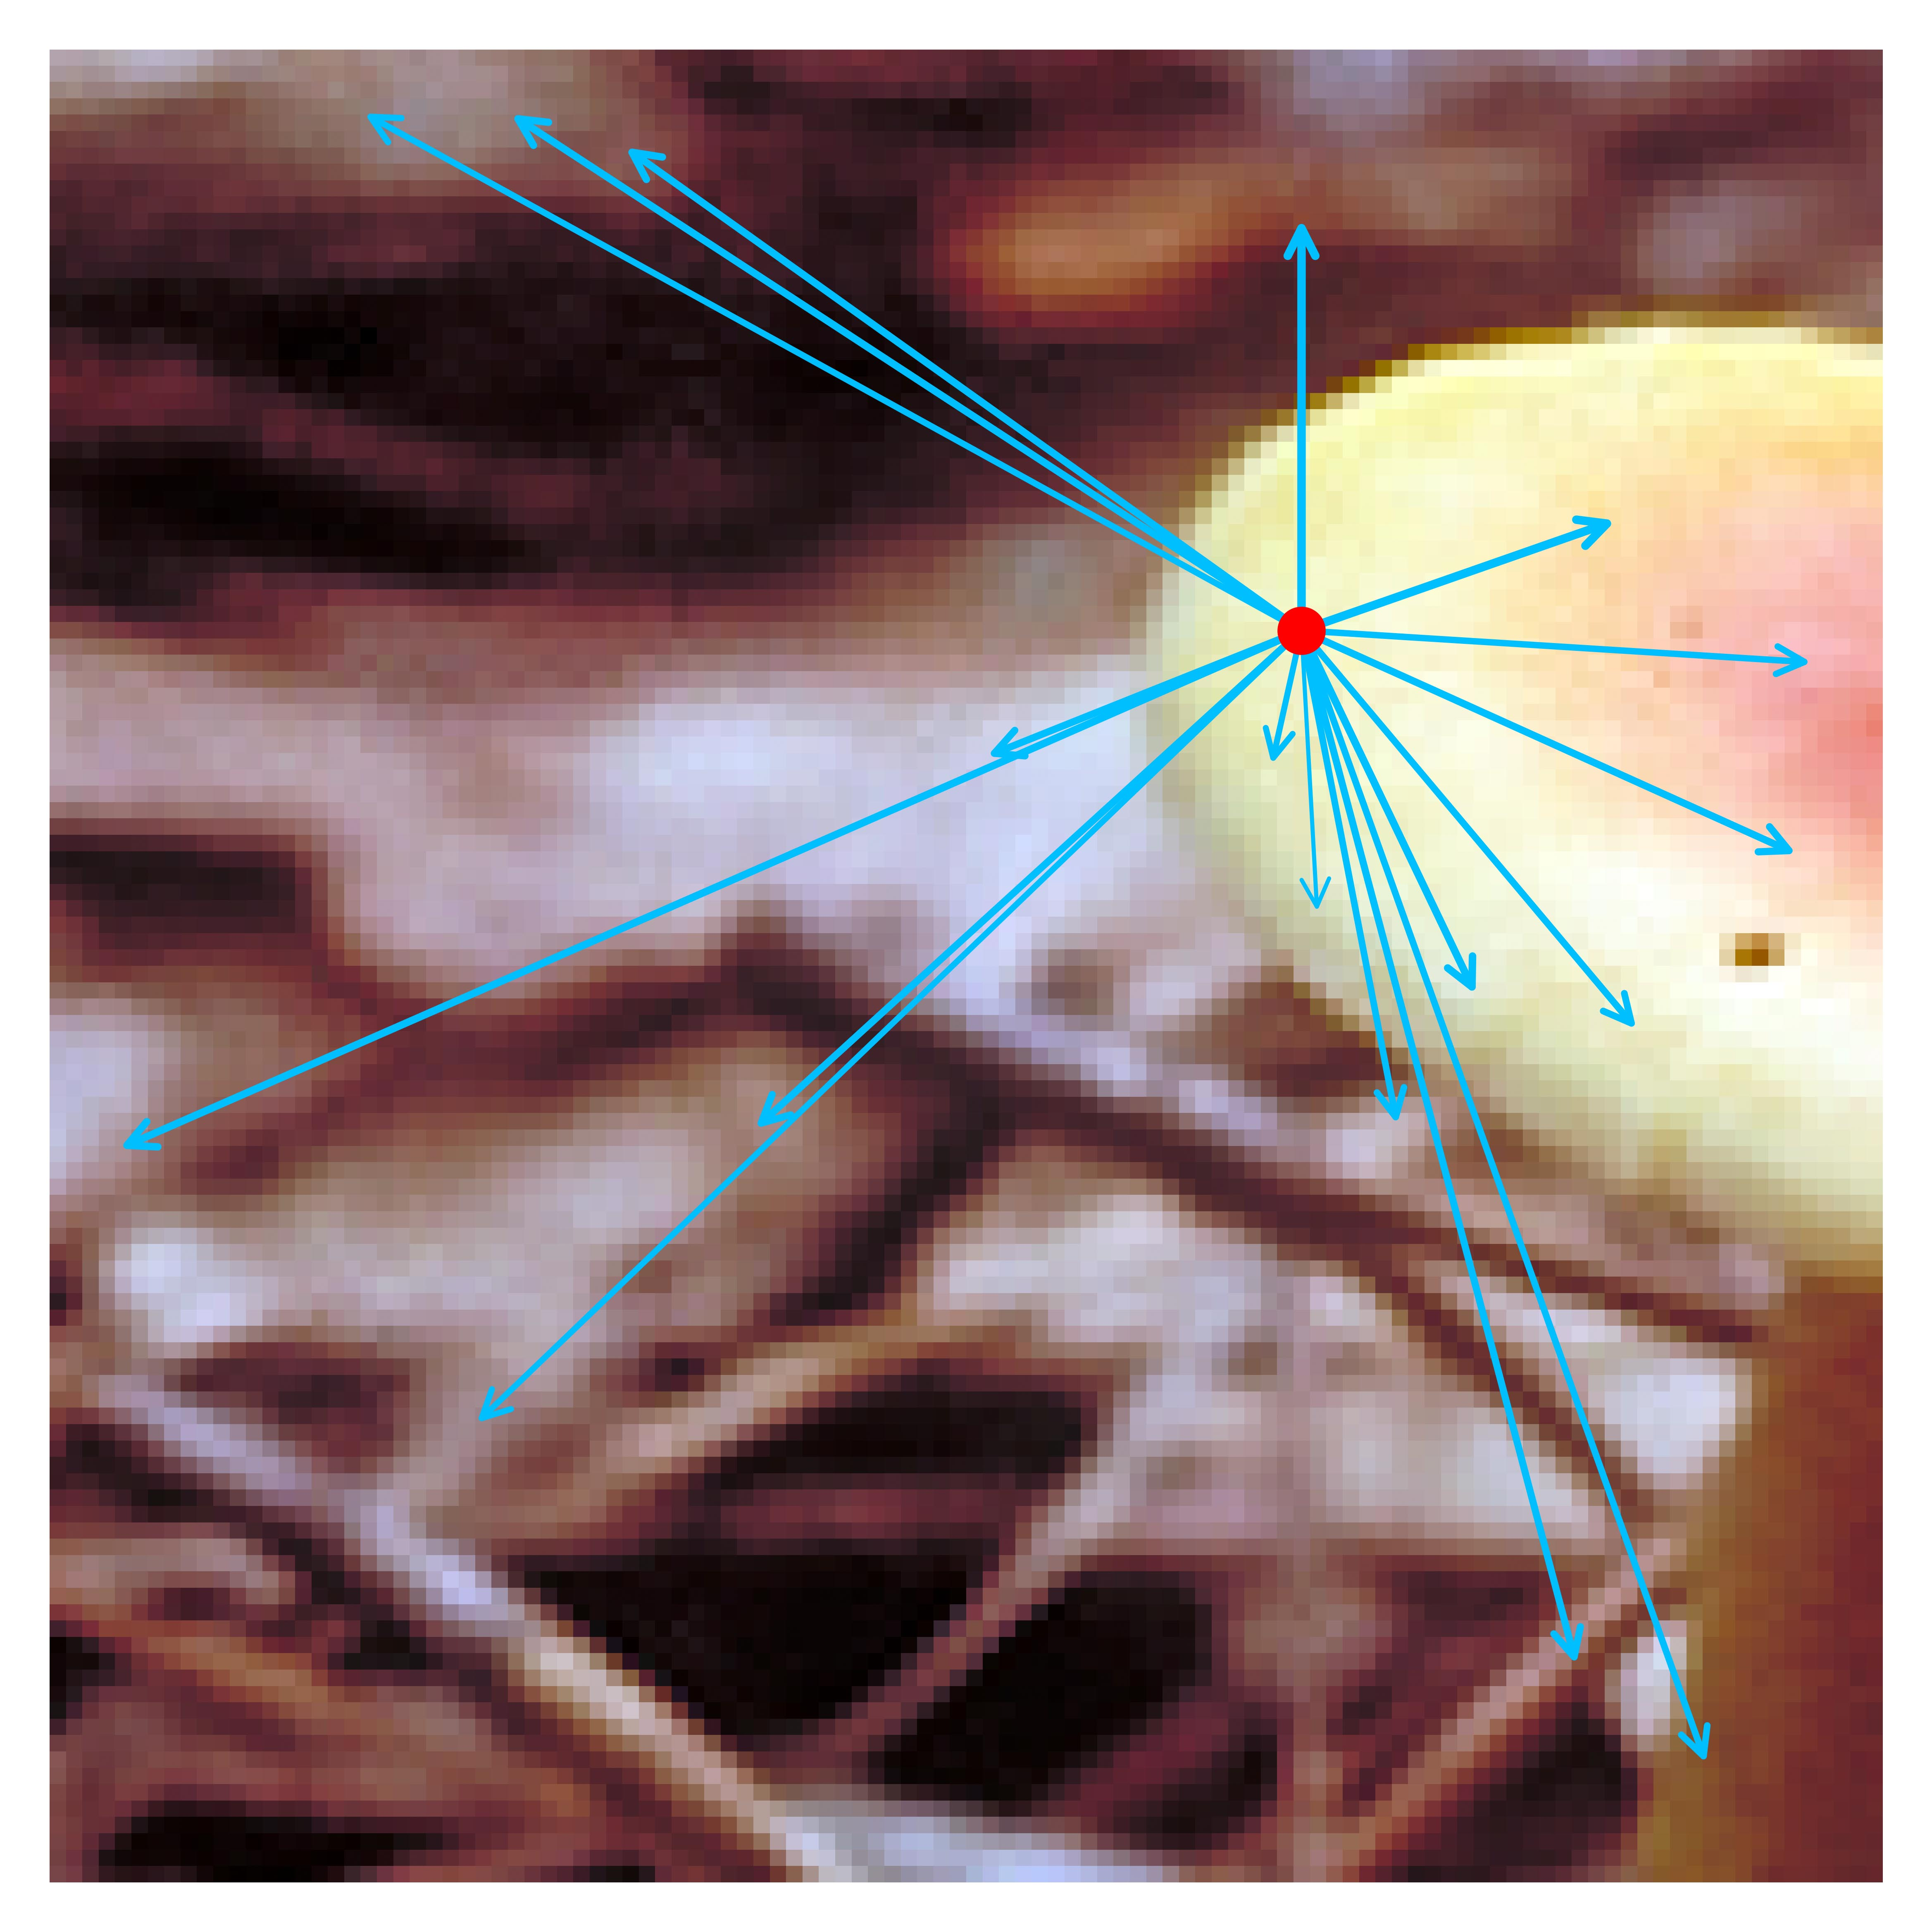
\includegraphics[width=1.5in]{cropped/shroom_superpixel_15.jpg}
			\centerline{(p)}
			\label{SHROOM-4}
		\end{minipage}
		\caption{Selected demonstrations of the non-local behavior and long-range dependencies with regard to the cropped image patches from the illustrated images. The details of Figure (a) to (p) are described in the thesis.}
		\label{Non-local Behavior of the cropped patches}
	\end{figure*}
	
	\reffig{Non-local Behavior of the cropped patches} demonstrates the non-local interactions in some images with size $112 \times 112$ cropped from~\reffig{Non-local Behavior from the TID2013 database}. The detailed descriptions of subfigures in~\reffig{Non-local Behavior of the cropped patches} are as follows: (a) The cropped plane image patch with a query on the jet head. (b) The cropped plane image patch with a query on the jet wings. (c) The cropped plane image patch with a query on the sky. (d) The cropped plane image patch with a query on the jet engine. (e) The cropped boat image with a query on the deep shade. (f) The cropped boat image patch with a query on the shallow shade. (g) The cropped boat image patch with a query on the sky. (h) The cropped boat image patch with a query on the boat. (i) The cropped Statue of Liberty image patch with a query on the lady's hand. (j) The cropped Statue of Liberty image patch with a query on the lady's hat tip. (k) The cropped Statue of Liberty image patch with a query on the lady's neck. (l) The cropped Statue of Liberty image patch with a query on the lady's arm. (m) The cropped shrooms image patch with a query on the stalk. (n) The cropped shrooms image patch with a query on the mushroom cap. (o) The cropped shrooms image patch with a query on the stalk near the ground. (p) The cropped shrooms image patch with a query on the edge of the stalk. As can be seen from these images, the query is semantically correlated with the relational content,~\eg, regions, objects, and pixels. By integrating image features into region features, object-to-pixel relations are encoded and comprehended. Overall, the non-local interactions are capable of modeling dependencies, geometries, and relations in the image, which are essential for semantics and content understanding.
	
	As a complement to CNN, the non-local modeling shows a great potential for semantics and content understanding, making a significant difference in CV tasks. Compared with traditional convolutions, first of all, the learned non-local features are nonlocalized, with the capability of long-dependency modeling over the whole image. As a result, the context information in the image can be better extracted. Secondly, the image's content is adaptively processed depending on the content. Thus, feature extraction is content-adaptive and flexible. Last but not least, the geometric structures and relations are also explored through the non-local information and long-range dependencies. Thus, the non-local modeling methods can be applied to supplement shortcomings of traditional convolutions. In addition, HVS perceives image quality with long dependency constructed among different regions, inspiring us to explore the non-local interactions in quality prediction.	
	
	\subsection{Effective Image-specific Prior}\label{Effective Image-specific Prior}
	Non-local features have been proven to be an effective image-specific prior to regularize the solution space of various ill-posed and under-constrained vision tasks, such as image generation~\citep{zhang2019self} and image restoration~\citep{buades2011non}. The prior also preserves general knowledge and common sense of nature and environment, reflecting the statistical properties of the world~\citep{girshick2011cardinal, ulyanov2018deep}. Therefore, the non-local features regularize the solution space of visual quality assessment, leading to robust and generalized visual quality assessment methods.